\chapter{Noise Subtraction with Neural Networks}
\label{chap:nohair}

\begin{refsection}

\section{Subtractable Noise}

The sub-100 Hz gravitational wave band is ripe with important sources for cosmology and astrophysics. Binary black holes at high mass or redshift broadcast significantly in the sub-100 Hz gravitational wave band, with a characteristic frequency
\begin{equation}
f_{\rm merger} \simeq 40\,\left(\frac{3}{1+z}\right)\left(\frac{100\,M_\odot}{M_{\rm tot}}\right)\,{\rm Hz},
\end{equation}
where $z$ is the cosmological redshift and $M_{\rm tot}$ is the total mass of the system. The inspiral portion of binary neutron star mergers, necessary for detecting early warnings of the mergers, also falls in the sub-100 Hz regime. 

Unfortunately, the Advanced LIGO (aLIGO) is not operating at the fundamental limit of its sensitivity in the important sub-100 Hz band. Figure 
\ref{fig:noiseBudget} 
shows the noise budget of aLIGO during its first observing run. The fundamental limit of the detector sensitivity is determined by the quantum (grey trace) and the thermal (blue trace) noise~\cite{Martynov:16}. The quantum and thermal noise only dominate the measured noise (red trace) above 100 Hz. In the 10-20 Hz band the measured noise (red trace) is nearly two orders of magnitude larger than sum of the quantum and thermal noise.

\begin{figure}[htbp]
   \centering
   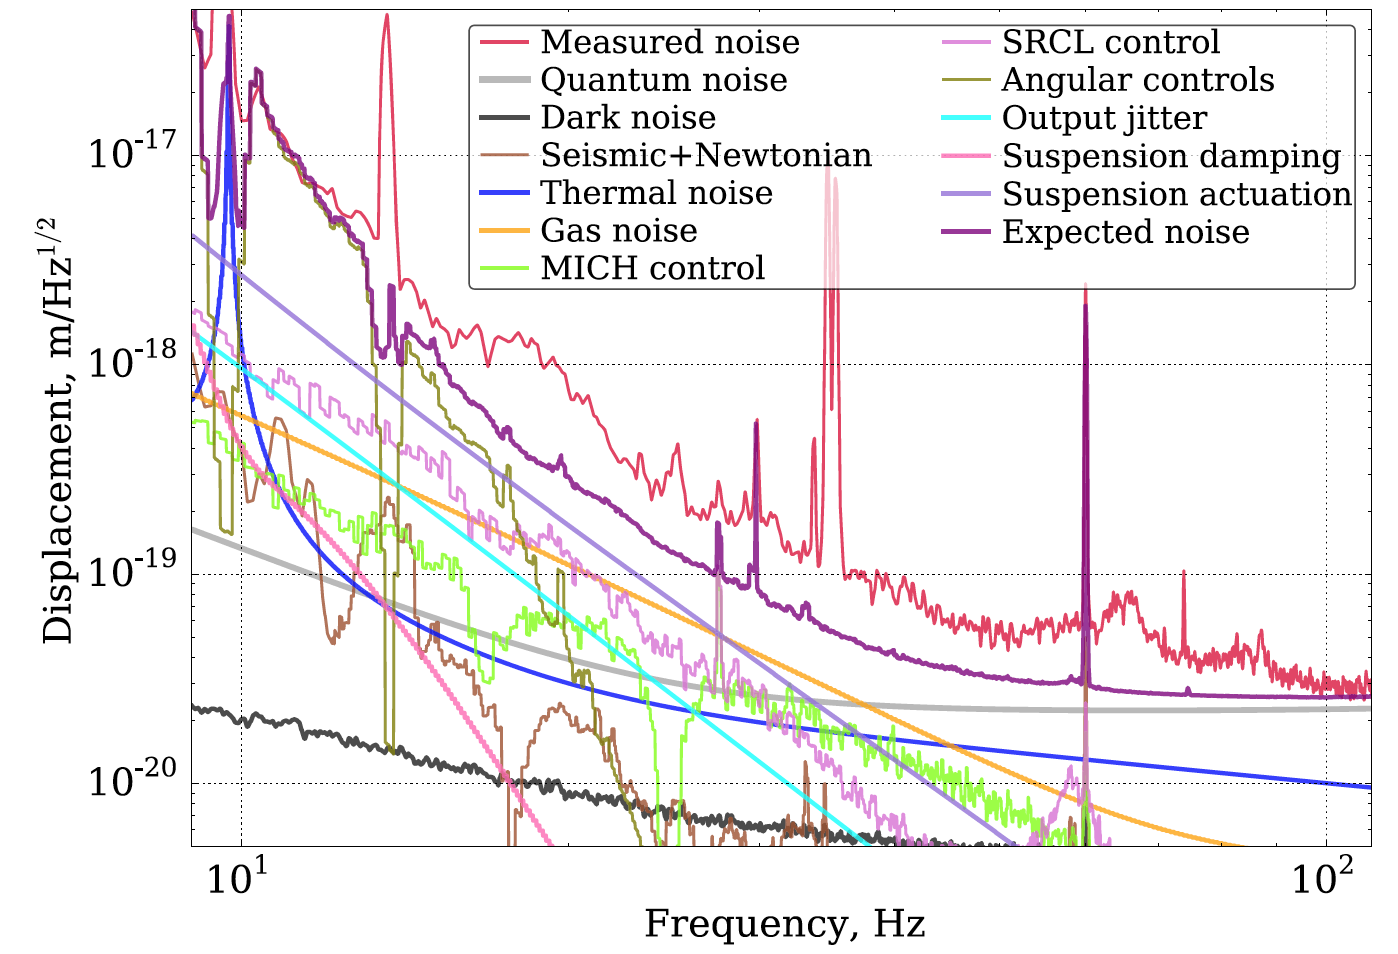
\includegraphics[width=\columnwidth]{chapter_noise_sub/etc/noiseBudget}
   \caption[Noise Budget]{Noise budget of aLIGO~\cite{Martynov:16}.
     In the sub-100 Hz band, the sensitivity is limited by subtractable noise sources since the measured noise is up to two orders of magnitude larger than the unsubtractable noise sources, the quantum and the thermal noise.}
   \label{fig:noiseBudget}
\end{figure}

The quantum and thermal noise is unsubtractable, meaning that there is no model (even in theory) that can predict them using auxiliary measurements of the detector. All other noise sources are subtractable, although the models necessary to predict them may be extremely complicated and difficult to deduce after constructing the detector. For example seismic perturbations and cross-couplings in the auxiliary control loops may contaminate the GW readout channel, ie the differential arm (DARM) length readout, via numerous different nonlinear coupling mechanisms.

\begin{figure}[htbp]
   \centering
   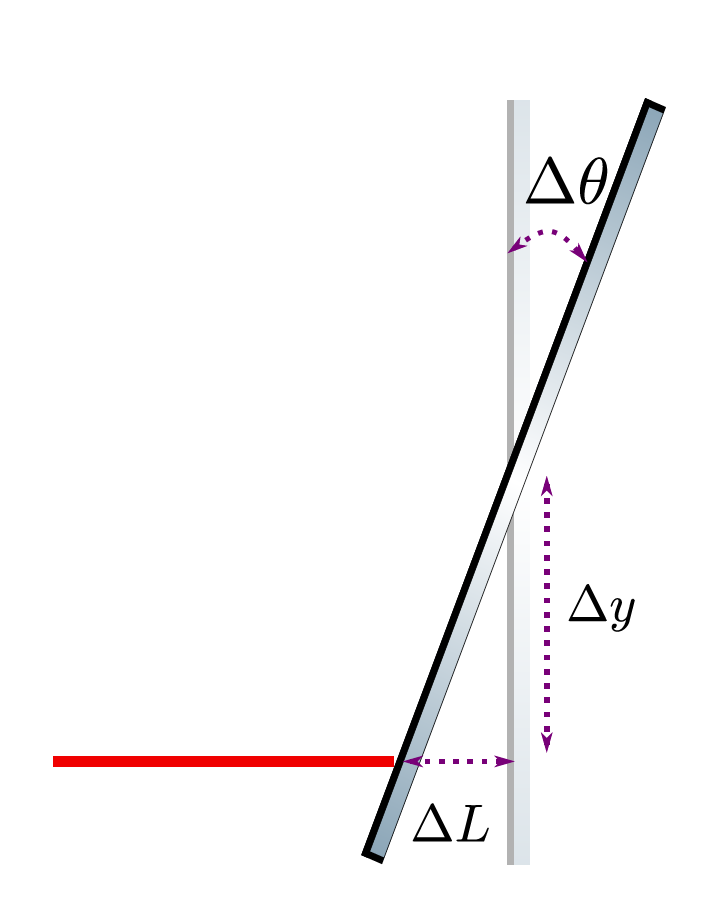
\includegraphics[width=0.28\columnwidth]{chapter_noise_sub/etc/a2l}
   \caption{Angle-to-length coupling~\cite{Yu:19}.}
   \label{fig:a2l}
\end{figure}

\begin{figure}[htbp]
   \centering
   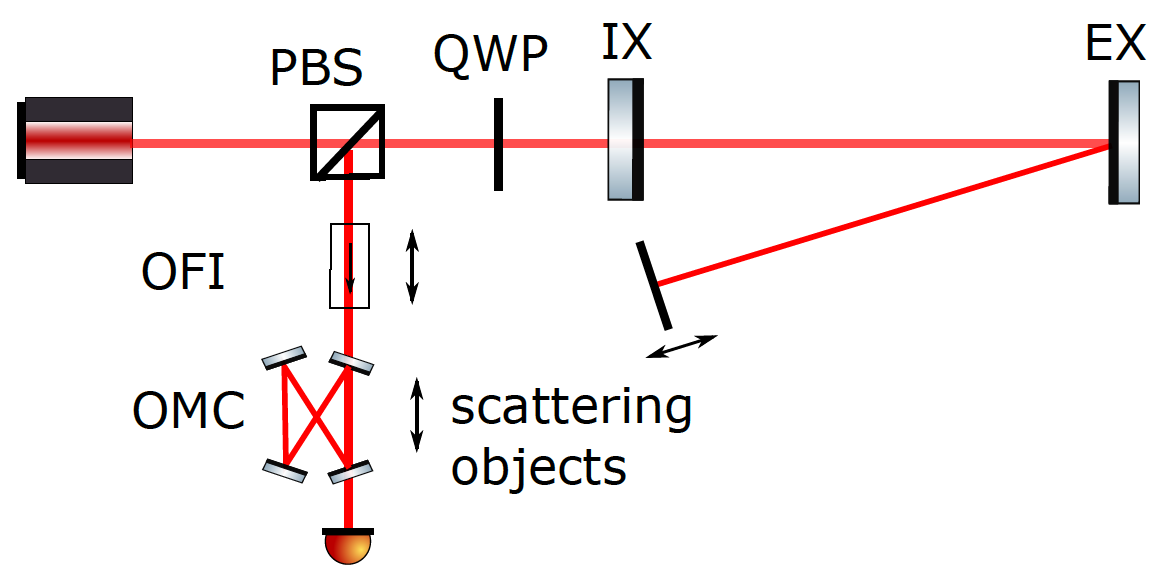
\includegraphics[width=0.6\columnwidth]{chapter_noise_sub/etc/scattering}
   \caption{Scattering noise coupling~\cite{Martynov:15}.} 
   \label{fig:scattering}
\end{figure}

%\begin{figure}[ht]

 % \begin{subfigure}{0.28\textwidth}
 %   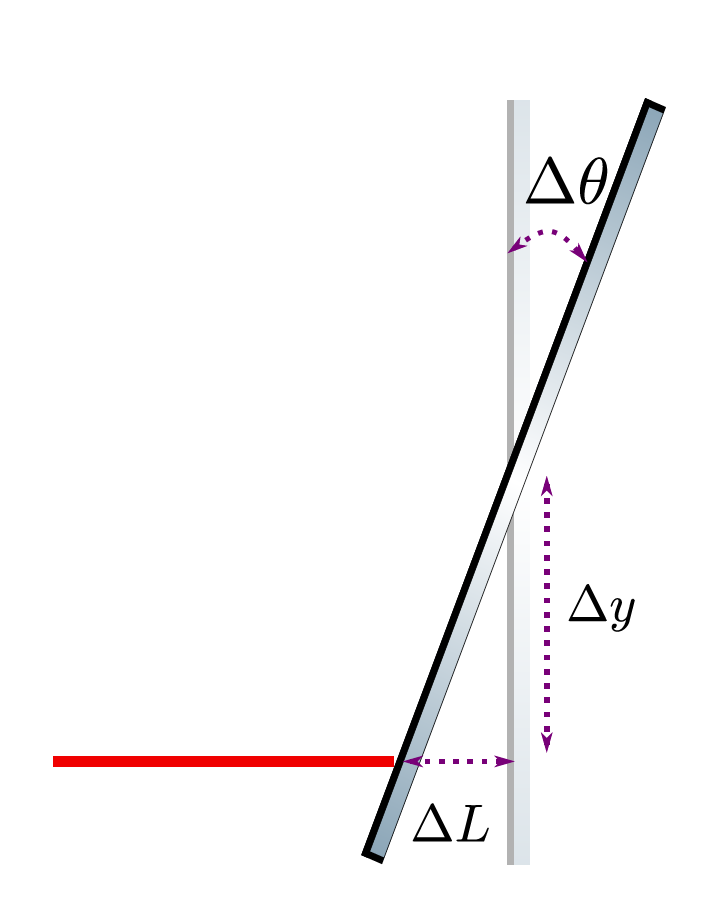
\includegraphics[width=\textwidth]{chapter_noise_sub/etc/a2l}
   % \caption{Angle-to-length coupling~\cite{Yu:19}.}
 %   \label{fig:a2l}
%  \end{subfigure}
%  \begin{subfigure}{0.6\textwidth}
%    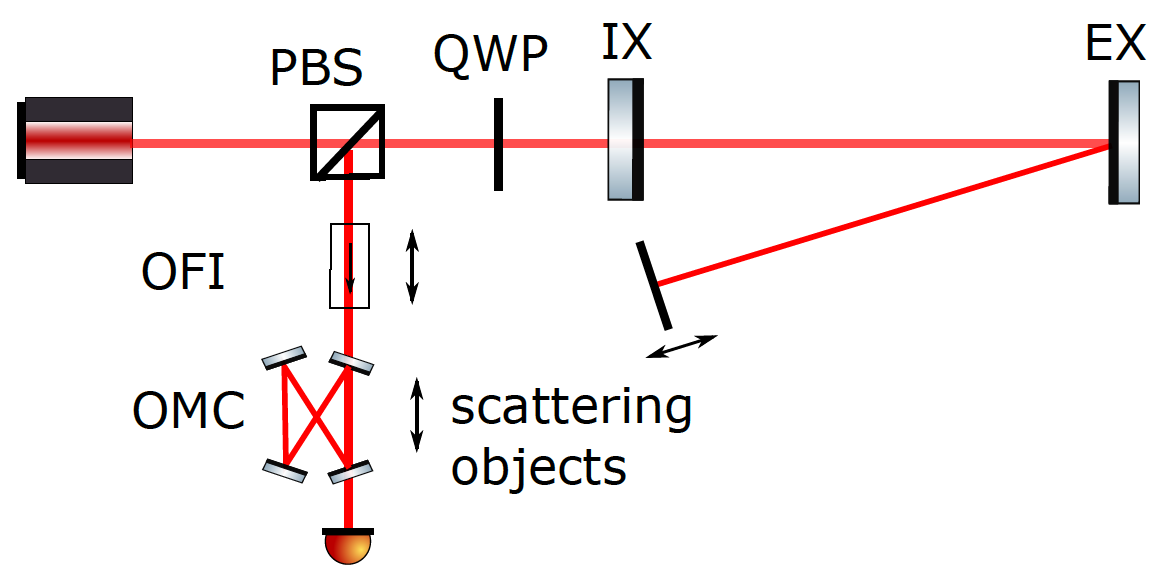
\includegraphics[width=\textwidth]{chapter_noise_sub/etc/scattering}
%    \caption{Scattering noise coupling~\cite{Martynov:15}. }
%    \label{fig:scattering}
%  \end{subfigure}

%\caption{Examples of nonlinear noise coupling in LIGO.}
%\label{fig:nl_coup}
%\end{figure}

For example, as shown in Figure 
\ref{fig:a2l}, 
angular motions in the mirror $\Delta \theta (t)$ couple bilinearly with displacements $\Delta y (t)$ in the beamspot from the rotational pivot to mimic a fluctuation in length $\Delta L (t)=\Delta\theta(t) \Delta y(t)$. As another example, shown in 
Figure \ref{fig:scattering}, 
stray light from the main beam can scatter off objects near the interferometer moving on seismic time scales and recombine with the main beam, producing light fields $\Delta E$ phase shifted from the main field by 
\begin{equation}
\sin \left[4\pi \frac{\Delta x(t)}{\lambda} \right],
\end{equation}
where $\lambda$ is the laser wavelength and $\Delta x(t)$ is the relative displacement between the mirror and the scattering objects. The scattered light fields $\Delta E$ can up-scatter the low-frequency seismic motion $\Delta x(t)$ into DARM. 

In both situations, monitoring auxiliary channels can allow us to subtract the noise they cause.  We often refer to these auxiliary channels as witness channels and the noise they cause as the target channel. For example in the bilinear noise mechanism, the spot displacement $\Delta y$ and the angular motion of the mirror $\Delta \theta$ are witnesses channels and the length change $\Delta L$ is the target channel. 

Our approach is to remove the subtractable noise offline by measuring auxiliary channels, processing them to calculate the subractable noise, and then removing it. Linear regression has been tried with some success \cite{lin_reg}, but since the couplings are nonlinear in nature, non-linear regression may lead to better performance. Neural networks are a form of non-linear regression that has had success in everything from image recognition \cite{10.1007/978-981-15-3020-3_23} to natural language processing \cite{FATHI2018229} to predicting financial markets \cite{siaminamini2018forecasting} (which is actually a somewhat similar problem to reducing the noise in DARM)

\section{Mock Data}

The real data poses a challenging problem both because it is realistic (and hence complicated) and the underlying mechanisms producing the subtractable noise are not all known. To best tailor our network to real interferometer data, we first ensure that we know how to regress simulated mock data, where we know exactly the nonlinearity and complexities that we are trying to model. 

Hence we start with very simple mock data and repeat these two steps until we can subtract noise for realistic mock data
\begin{itemize}
\item find a network structure that performs well on the current set mock data
\item make mock data more realistic, potentially rendering previous network structure inadequate
\end{itemize}

\subsection{Frequency Dependent Filtering}
The auxiliary channels which we use as witnesses are often measured in digital counts rather than physical units. To get physically relevant quantities like the longitudinal or angular motion of the mirror requires frequency dependent filtering. In other cases, the quantity that couples nonlinearly into DARM differs from the measured witness by a transfer function, e..g the angular motions of the mirrors differ from the their witnesses, the acs control signals, by a $1/f^4$ transfer function for the mirror suspension. 

It is important that our network can learn these filters both for simplicity and because we can not account for all the filtering in the interferometer. Our simplest mock data ensures that we can handle these filters and is 
\begin{equation}
y(t)=H[x(t)],
\end{equation}
where $y$ is the target, $x$ is the witness, and $H$ is a bandstop or bandpass buttersworth filter.


\subsection{Bilinear Coupling}
Motivated, by the angle-to-length mechanism, we consider mock data with a N pairs of bilinearly coupled, perfect witnesses
\begin{equation}
y(t)=\sum_{i=1}^N x_i(t) x_{N+i}(t)
\end{equation}
where $y$ is the target and $x_i$ are the witnesses.

We start with $x_i$ that  have white spectra and then make the mock data progressively more challenging giving them colored spectra representative of the beam spot motion and angular position of the mirrors, adding white sensing noise to each witness and adding background noise (sampled from the aLIGO noise curve) to the target. We will refer to this mock data set as the colored bilinear mock data.

Finally in our most realistic bilinear mock dataset.  we try to model the angle-to-length noise as it occurs in aLIGO. We will refer to this mock data set as the bilinear ifo mock data.

There are 2 mirrors in each arm of the interferometer. The spot position on each mirror has two degrees of freedom (i.e pit and yaw on each mirror) and the angular motion of each mirror has 2 degrees of freedom (i.e pit and yaw on each mirror), so there are 16 perfect witnesses.

To determine the coupling to DARM, we decompose the mirror spot positions into a common/differential and hard/soft mode basis (see \cite{Dooley:13,SIDLES2006167,LIGO:2015} for a description of hard/soft modes). Similarly, we decompose the angular motion into the common/differential, hard/soft basis. For geometric reasons, the soft modes can essentially be filtered out by control loops and we consider only the hard modes to couple to DARM $y(t)$; we take the coupling to be hard*hard and c*d
\begin{equation}
y(t)=x^{spot}_{c, p}x^{angle}_{d,p}(t)+x^{spot}_{d, p}x^{angle}_{c,p}(t)+x^{spot}_{c, y}x^{angle}_{d,y}(t)+x^{spot}_{d, y}x^{angle}_{c,y}(t),
\end{equation}
where the hard modes $x$ are labeled with c/d  for common/differential, p/y for pitch/yaw, and angle/spot to distinguish between the angular and spot position true motion.


We will not have access to the perfect witnesses to perform the regression.

The true angular motion and true spot motion can (in theory) be reconstructed from the Alignment Sensing and Control (ASC) system measurements and Internal Seismic Isolation (ISI) system measurements. We use our knowledge of the these systems to model the witnesses in our most realistic bilinear mock dataset.

The ASC system is the control system responsible for maintaining the mirror alignment at high frequencies. The angle witnesses are essentially ASC error signals measuring the hard and soft modes of the mirror rotation, which differ from the true angular motion by  a $1/f^4$ transfer function for the suspension. In our mock data, we model the ASC error signals by giving them a few known resonances and most of their power at high frequencies. To get the witnesses for the ASC channels, we also multiply by a fixed, unknown mixing matrix to account for unknown cross coupling during the measurement of the error signals and add a small amount of white measurement noise.

The ISI system is the control system responsible for removing low frequency seismic motion from the test masses. Movement of the objects holding the test mass, such as the suspension, couples into angular motion of the mirrors, which also produces beam spot motion. In our mock data, we model ISI channels by giving them a few known resonances and most of their power at low frequencies. We model the true spot position as a linear combination of the eight ASC error signals (again multiplied by a different mixing matrix to model cross couplings and supplemented with white measurement noise) and eight ISI channels (supplemented with measurement noise) plus and unknown DC offset. It is not immediately obvious which ISI channels will be necessary for reconstructing the true spot position so we also include eight irrelevant ISI channels that our network will have to learn to discard.

Hence, the coupling in this model is essentially between low frequency ISI signals and high frequency ASC signals, the coupling between two high frequency ASC signals will be not effect the target band (10-20 Hz) in DARM that we are trying to clean. This is also why we didn't also give the true angular motion a low frequency ISI component; the coupling between two low frequency ISI signals is not in the 10-20 Hz band.

%We take the spot motion to be a linear combination of 8 asc error signals and 8 isi channels, which are characterized by different spectral shapes and resonances, plus an unknown dc offset. To get the witnesses for the asc channels, we multiply by a fixed, unknown mixing matrix to account for unknown cross coupling during the measurement of the error signals and add a small amount of white measurement noise.
%The witnesses for the isi channels include the 8 isi channels used to construct the true spot motion (plus a small amount of measurement noise) and 8 irrelevant isi channels that our network will have to learn to discard.


%The angle witnesses are essentially asc control signals which differ from the true angular motion by  a $1/f^4$ transfer function for the suspension. The difference between the angle witnesses and the asc control signals is again a mixing matrix and a small amount of measurement noise.

\section{Neural Networks}

\subsection{Notation}
We provide a brief review of the relevant elements of neural networks. An excellent introduction can be found in \cite{nielsen2015neural}.

Science is based on the fact that many variables in nature are related, given a set of independent variables (often referred to as features) $x$ it is possible to predict a set of target variables $y$. Linear regression assumes a linear relationship, i.e $y=wx$, where if $y$ is a N dimension vector of targets and $x$ is an M dimensional vector of features, $w$ is $N \times M$ matrix of coefficients that will be optimized by the regression algorithm.

Most functions are not linear, but are well approximated by linear functions over restricted regimes, so linear regression is useful in a wide range of problems. However, when the underlying relationship between $y$ and $x$ is significantly nonlinear over the domain of $x$, neural networks can outperform linear regression.

In neural network with no hidden layers, the output of the neural network is $z=\sigma(wx+b)$ where sigma is a fixed, nonlinear activation function, such as a sigmoid function $f(z)=1/(1+\exp(-z))$, $w$ is again $N \times M$ weight matrix learned by the regression, and $b$ is an N dimensional bias vector, also learned by the regression. This notation is vectorized, meaning that the activation function $\sigma$ is applied to each element of the vector.

\begin{figure}[htbp]
   \centering
   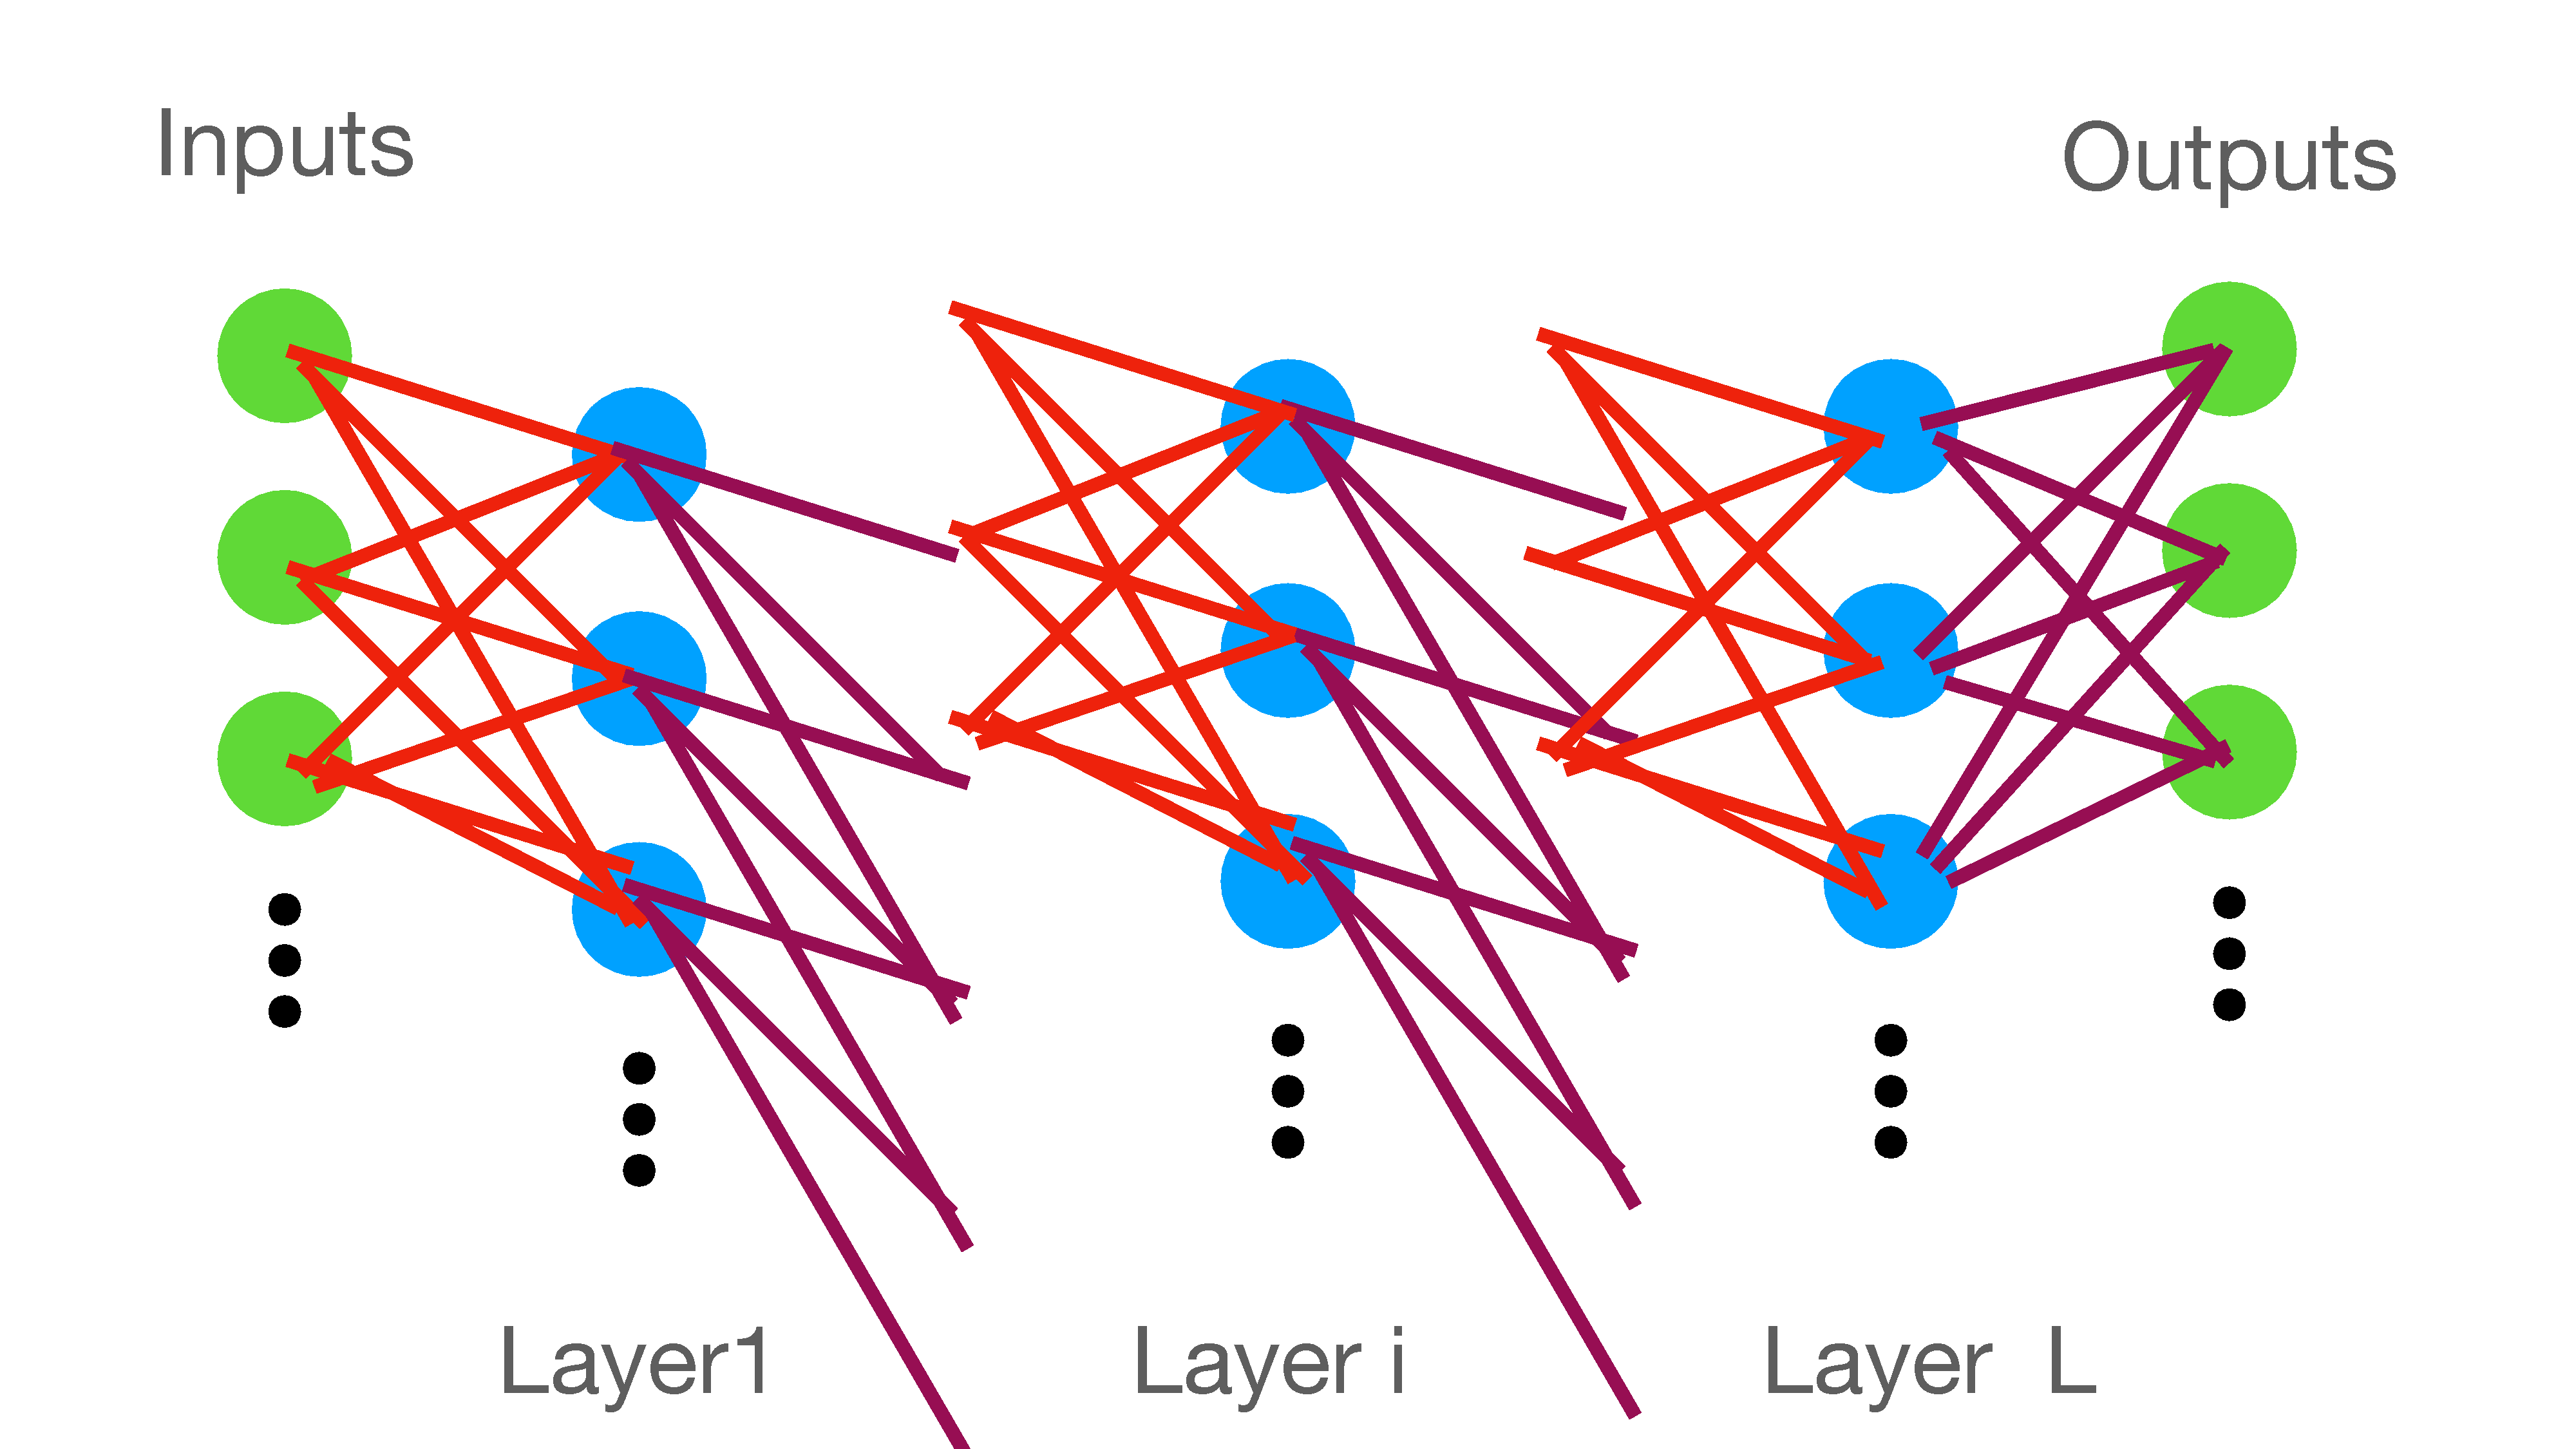
\includegraphics[width=\columnwidth]{chapter_noise_sub/etc/net_fig_cartoon}
  \caption{Each element of the vector z is represented by a node and each element of the weight matrix w is represented by a connection between nodes.}
   \label{fig:net_fig_cartoon}
\end{figure}

In deep learning, neural networks have one or more hidden layers as shown in figure \ref{fig:net_fig_cartoon}. In this case the output of the $i^{\rm th}$ hidden layer is $z^{i}=\sigma^{i}(w^{i}z^{(i-1)})+b^{i}$. If there are L layers, then the L weight matrices $w^1, \cdots w^L $ and L bias vectors $b^1, \cdots b^L $ are learned by the regression. As suggested by the notation, it is also common for each layer to have a different activation function. Referring to the figure each, element of the output $z^i$ is represented by a node and each element of weight matrix $w^i$ is represented by lines between nodes.

\subsection{Network Evaluation}
To evaluate the performance of a neural network it is necessary to split your dataset into three groups: training data, validation data, and testing data.
As described below, the training data is used to optimize the weights matrices and bias vectors. Neural networks often have thousands of free parameters and a common issue is overfitting. To avoid this pitfall, network performance is optimized on the testing data. A typical training algorithm involves a plethora of hyperparameters, such as the learning rate and various regularization parameters. To avoid overfitting by tuning these hyper parameters, the best values are determined by evaluation on the validation data.
\subsection{Optimization}
Most commonly, neural networks learn the weight matrices and bias vectors by optimizing a cost function $C(v)$ using a form of gradient descent. The most common cost function is Mean Squared Error (MSE):
\begin{equation}
C(v)=\text{mean}\left(\sum_{i=0}^{L}\left(y_{target}^i-y_{prediction}^i(v)\right)^2\right),
\end{equation}
where the network is trying to predict L targets $y_{target}^1, \cdots, y_{target}^L$, the mean is taken over all examples in the training set, and $v$ denotes a vector of weights and biases. The most common algorithm to optimize the cost function is stochastic gradient descent. In regular gradient descent, the gradient of the cost function with respect to the weights $\nabla_v C$ is calculated and the weight are updated as
\begin{equation}
v\to v-\eta \nabla_v C,
\end{equation}
where $\eta$ is a hyper parameter called the learning rate. In practice, in can be computationally intensive to calculate the gradient over the full training set of examples, so the stochastic gradient descent algorithm approximates the full gradient by  the gradient computed over a subset of training set examples, known as a mini-batch. Other minor modifications, such adding a momentum term \cite{DBLP:journals/corr/abs-1206-5533} \cite{Hinton2012}, are used in conjunction with the gradient descent algorithm.

\subsection{Regularization}
A neural network almost always has far more free parameters than data points in the training data. To avoid overfitting, several forms of regularization are used. 

Dropout layers \cite{JMLR:v15:srivastava14a} set a random fraction $x$ of the input weights to zero during each epoch of training. The remaining weights are calculated during training and then eventually scaled by $(1-x)$ when the network is used to make predictions. The idea is that reliance on a few very large weights is symptom of overfitting and the drop out layers prevent this reliance from occurring. The fraction $x$ is a hyper parameter that needs to be tuned with the validation data.

Another form common form of regularization is $\ell^2$ regularization where the same of the squares of the N weights $\lambda \sum_{i=0}^N w_i^2$ is added to the cost function, where $\lambda$ is a hyper parameter tuned with the validation data. Again, the idea is that the extra term discourages large values of the weights, which is a symptom of  overfitting.

\subsection{Convolutional Layers}
A key element of our noise subtraction problem is that in the "true noise" model, frequency dependent filters are also applied to the channels which nonlinearly mix and contaminate DARM. Hence in order to subtract this noise, our network needs have connections between nodes at different times. This is accomplished with 1D convolutional layers \cite{KIRANYAZ2021107398}. 

A convolutional layer is specified by two hyper parameters: the filter number and the kernel size. Let's say the output of the previous layer has shape (number of timesteps, number of channels), then the output of the convolutional layer will have shape (number of time steps, filter number). The kernel dictates how far back in time nodes at different times will be connected; there will be connections between nodes separated in time by less than the kernel.  Convolutional layers work best with stationary data, so the weights between nodes separated by the same amount of time are taken to be the same (as long as they are between the same input and output channel).

\subsection{Equation Learning Layers}
Equation learning (EQL) layers are useful for learning physical models \cite{kim2020integration}. Each node in the equation learning layer has a (potentially different) activation that is common in physical models. In our EQL layers, we have five unary activation functions: the identity function, $x**2$, $\sin(x)$, $\cos(x)$, and $elu(x)$, as well as one binary activation function $x_1*x_2$. Since the EQL often contains the exact non-linearity that occurs in the underlying process that is being learned, ideally most of the weights in the EQL layer will be driven to zero, leaving only a few non-negligible weights. To accomplish this, we always use a smoothed $\ell^{0.5}$ norm to regularize the weights in the EQL layer.
Hence there are three hyper parameters that determine the EQL layer: the number of nodes that has each unary activation function, the number of pairs of nodes for each binary activation function, and the weight for the $\ell^{0.5}$ regularization.

\section{Mock Data Results}

All of our results are obtained using Keras \cite{chollet2015keras}.

\subsection{Frequency Dependent Filtering}

Our simplest mock data set consisting of a single feature that is filtered with a buttersworth bandstop filter to produce the target, provides an important conceptual consideration; we need to include convolutional layers with linear activation functions to learn unmodeled frequency-dependent filtering. 

Figure \ref{fig:bandstop_ASD} llustrates the successful subtraction by showing the amplitude spectral densities of the target, prediction, and residual. Outside the bandstop, we achieve roughly a factor of 100 reduction between the target/neural network prediction and the residual between the target and prediction.
The network used to achieve this subtraction, shown in Figure \ref{fig:bandstop_net}, consists of a single convolutional layer (with a kernel of half a second) regularized with a dropout layer.

\begin{figure}[htbp]
   \centering
   \includegraphics[width=\columnwidth]{chapter_noise_sub/etc/Filter_spectra}
   \caption{Amplitude Spectral densities illustrating subtraction for a bandstop filtering mock data. Outside the bandstop, we achieve roughly a factor of 100 reduction between the target/neural network prediction and the residual between the target and prediction}
   \label{fig:bandstop_ASD}
\end{figure}

\begin{figure}[htbp]
   \centering
   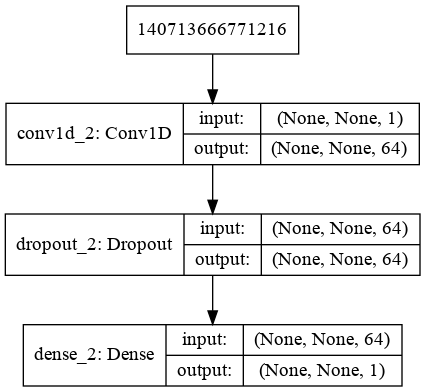
\includegraphics[width=0.7\columnwidth]{chapter_noise_sub/etc/bandstop_net}
  \caption{Network schematic for successful network on bandstop filtering mock data.}
   \label{fig:bandstop_net}
\end{figure}

\subsection{Colored Bilinear}
We have success solving the colored bilinear mock data with a simple four layer dense network depicted in Fig \ref{fig:net}.
The nonlinearity is captured by a selu activation function in the middle layers and the network is regularized with alternating dropout layers. 
The target and the  fast (ie the high frequency ASC) witnesses are whitened in ordered to handle the large dynamic range.
The network is trained using a version of stochastic gradient descent called Nesterov-accelerated Adaptive Moment Estimation (Nadam) and employes a learning rate schedule and early stopping.


\begin{figure}[htbp]
   \centering
   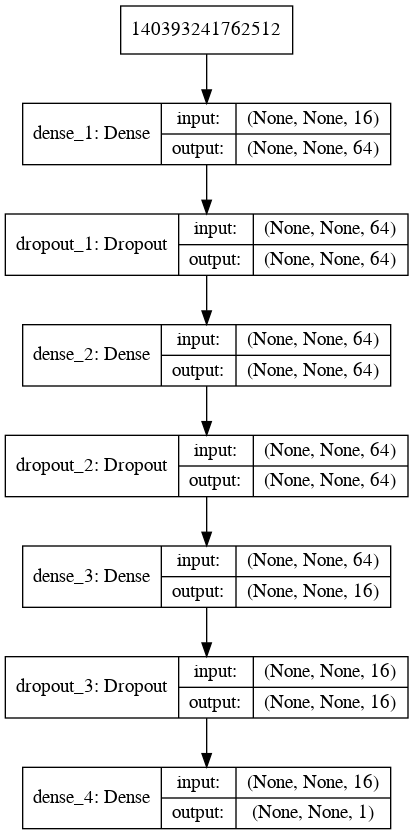
\includegraphics[width=.7\columnwidth]{chapter_noise_sub/etc/net_diag}
   \caption{Schematic diagram of network used to solve the Colored Bilinear Mockdata with 16 pairs}
   \label{fig:net}
\end{figure}

%We show results for 2,4,8,16, and 32 pairs of witnesses. Fig \ref{fig:ASD1} shows that we successfully reduce the noise by approximately a factor of 10 in the 10-20 Hz band for 2,4, and 8 pairs, while Fig \ref{fig:ASD2} shows that the success wanes for 16 pairs and completely disappears for 32 pairs. This is not necessarily a fundamental issue with the network and could possibly be alleviated with some hyper parameter tuning as the loss plotted in Fig \ref{fig:loss2} reveals that learning is initially relatively very slow for 16 and 32 pairs compared to the learning for 2,4, and 8 pairs, which is shown in Fig \ref{fig:loss1}. 

We show results for 1,2,4, 8,16, and 32 pairs of witnesses. We find decreasing effectiveness as the number of pairs increases. Fig \ref{fig:ASD1} shows that we successfully reduce the noise by approximately a factor of 10 in the 10-20 Hz band for 2,4, and 8 pairs, while Fig \ref{fig:ASD2} shows that the success wanes for 16 pairs and completely disappears for 32 pairs. This is not necessarily a fundamental issue with the network and could possibly be alleviated with some hyper parameter tuning as the loss plotted in Fig \ref{fig:loss2} reveals that learning is initially relatively very slow for 16 and 32 pairs compared to the learning for 2,4, and 8 pairs, which is shown in Fig \ref{fig:loss1}. 

\begin{figure}[htbp]
   \centering
   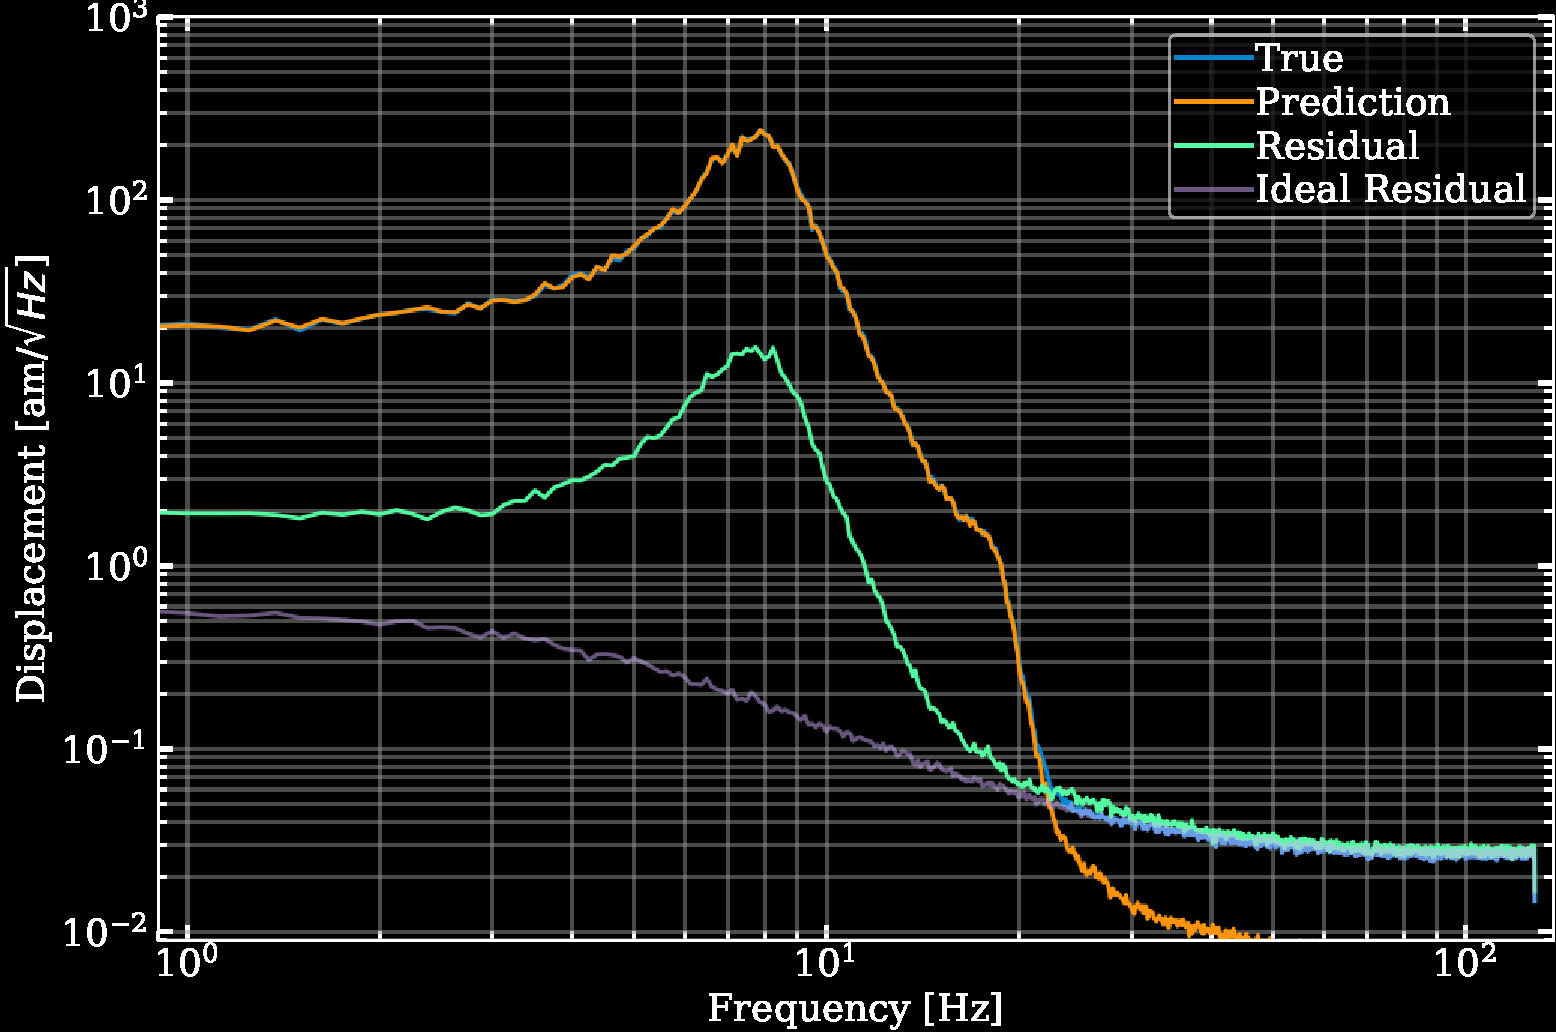
\includegraphics[width=.7\columnwidth]{chapter_noise_sub/etc/spectra1C}
    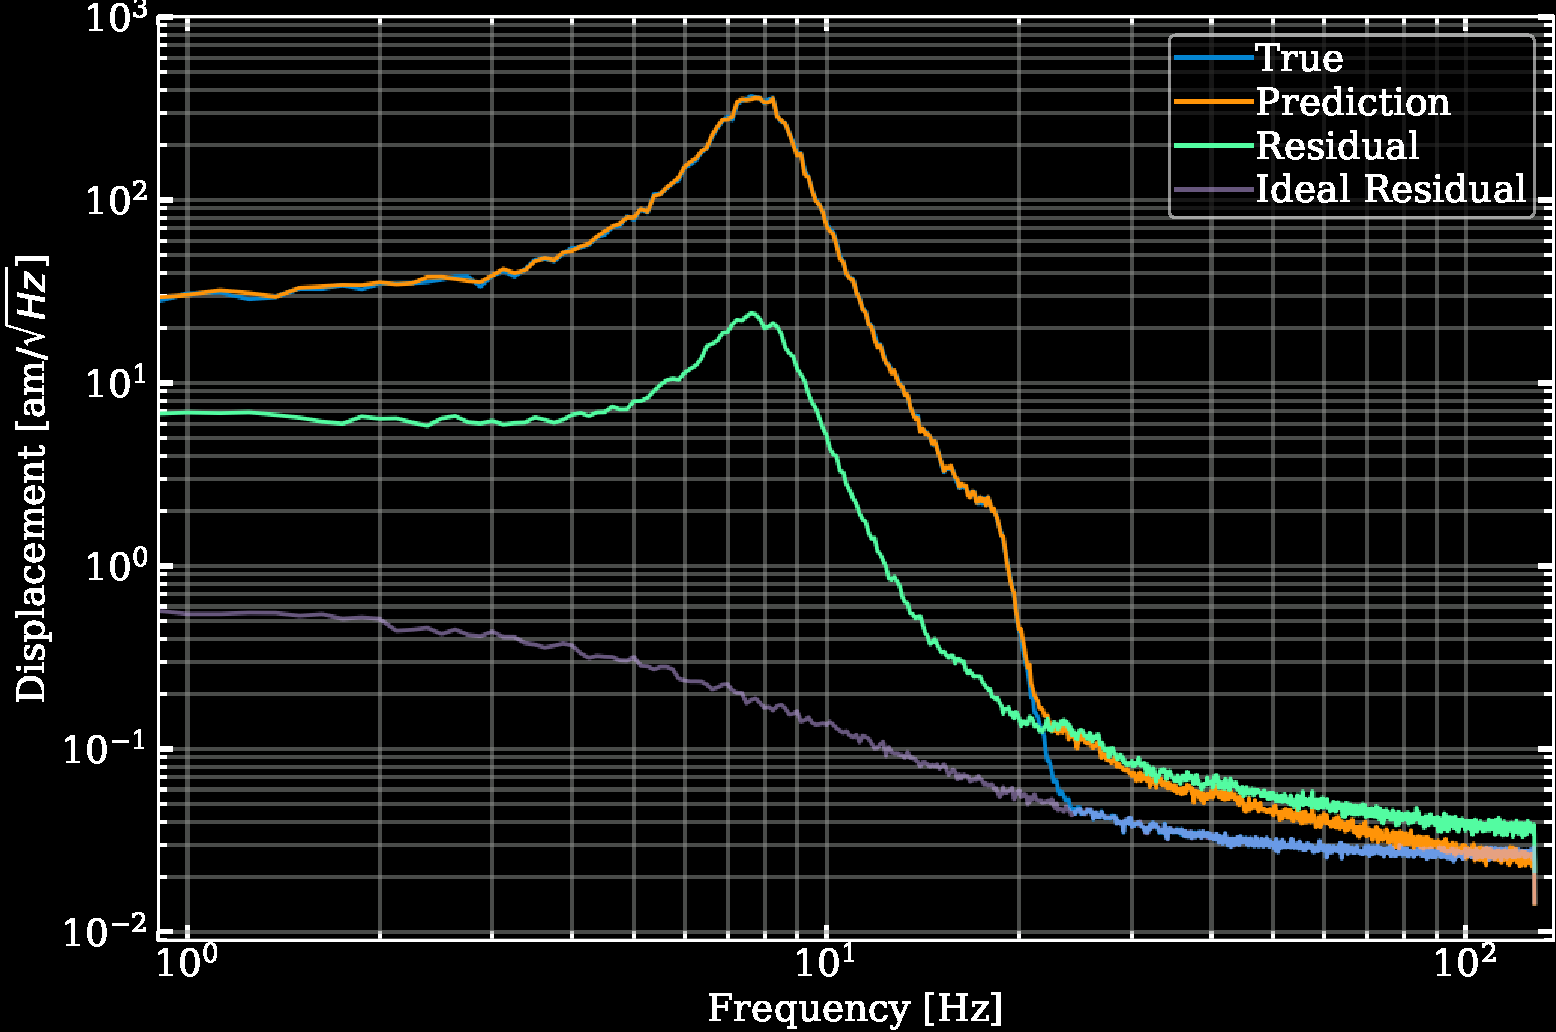
\includegraphics[width=.7\columnwidth]{chapter_noise_sub/etc/spectra2C}
     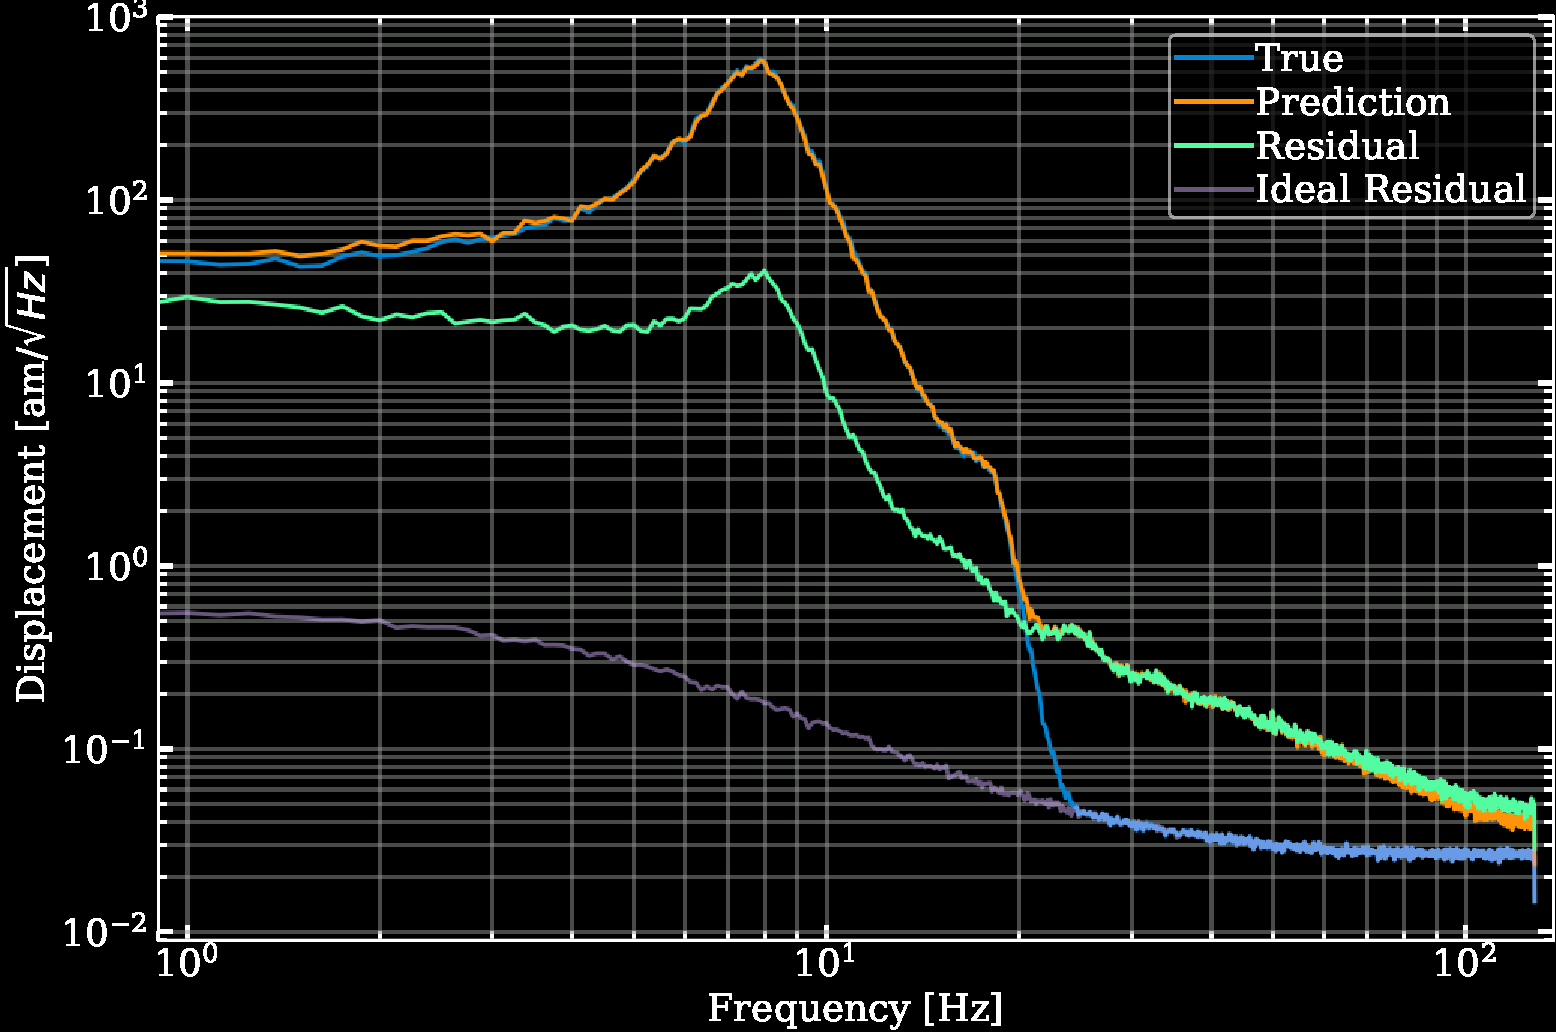
\includegraphics[width=.7\columnwidth]{chapter_noise_sub/etc/spectra4C}
   \caption{Amplitude Spectral densities illustrating subtraction for the colored bilinear mock data with 1 (top panel), 2 (middle panel), and 4 (bottom panel) pairs. At 10 Hz, we achieve a factor of 20 reduction (1 pair)}
   \label{fig:ASD1}
\end{figure}

\begin{figure}[htbp]
   \centering
   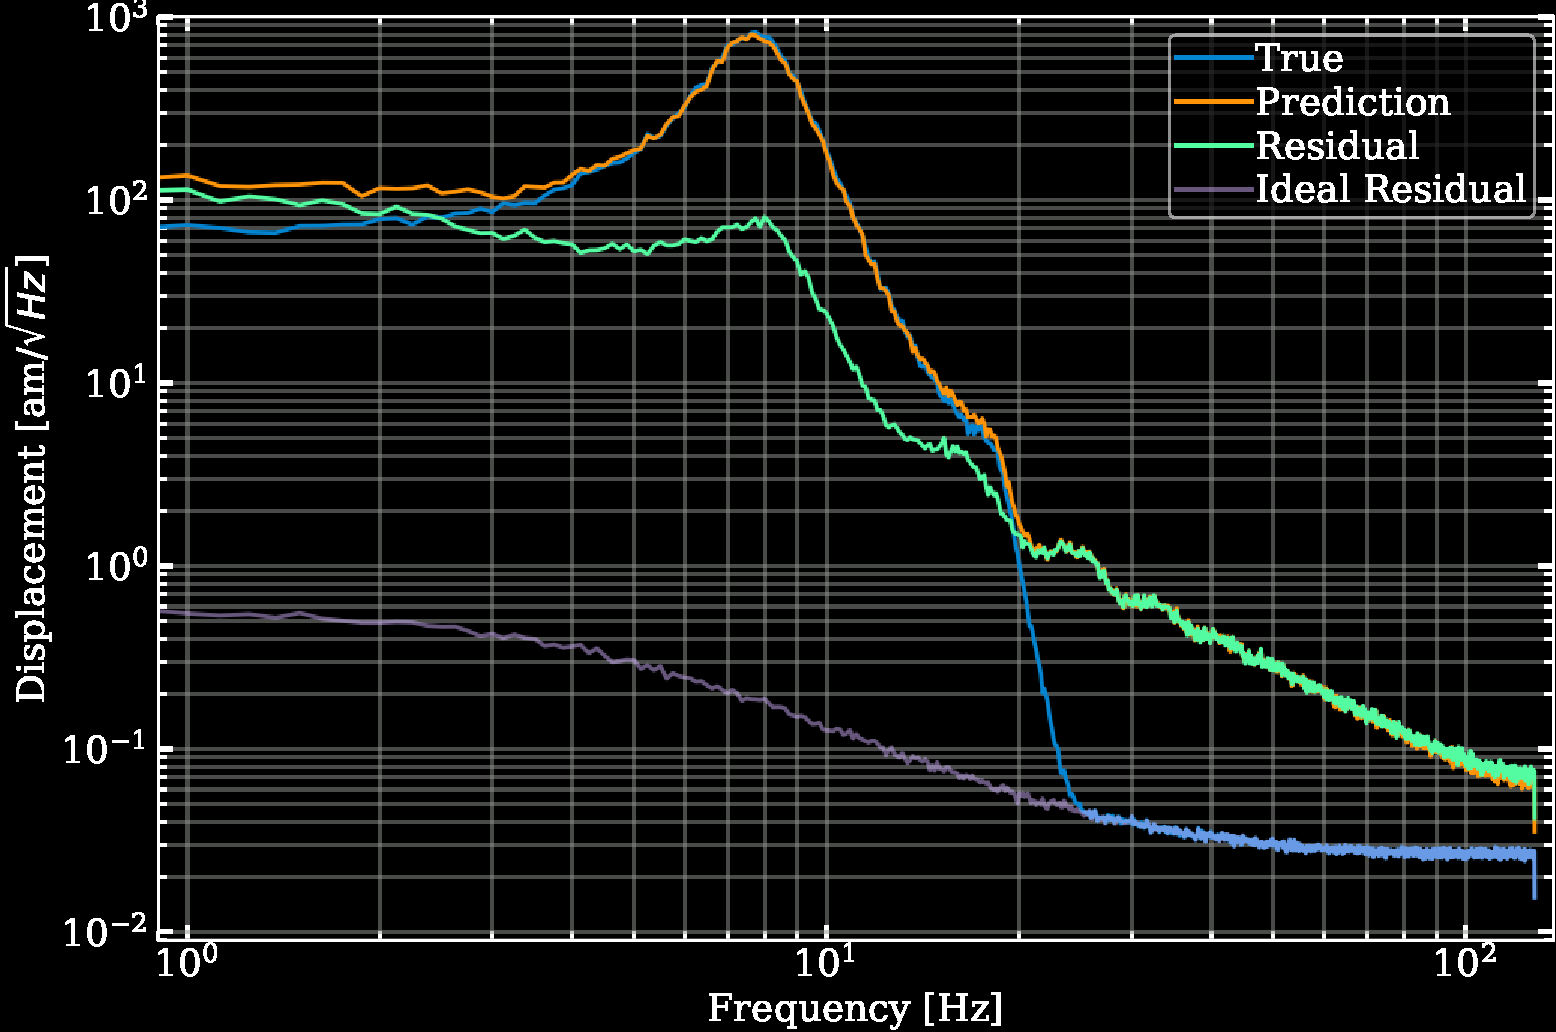
\includegraphics[width=.7\columnwidth]{chapter_noise_sub/etc/spectra8C}
    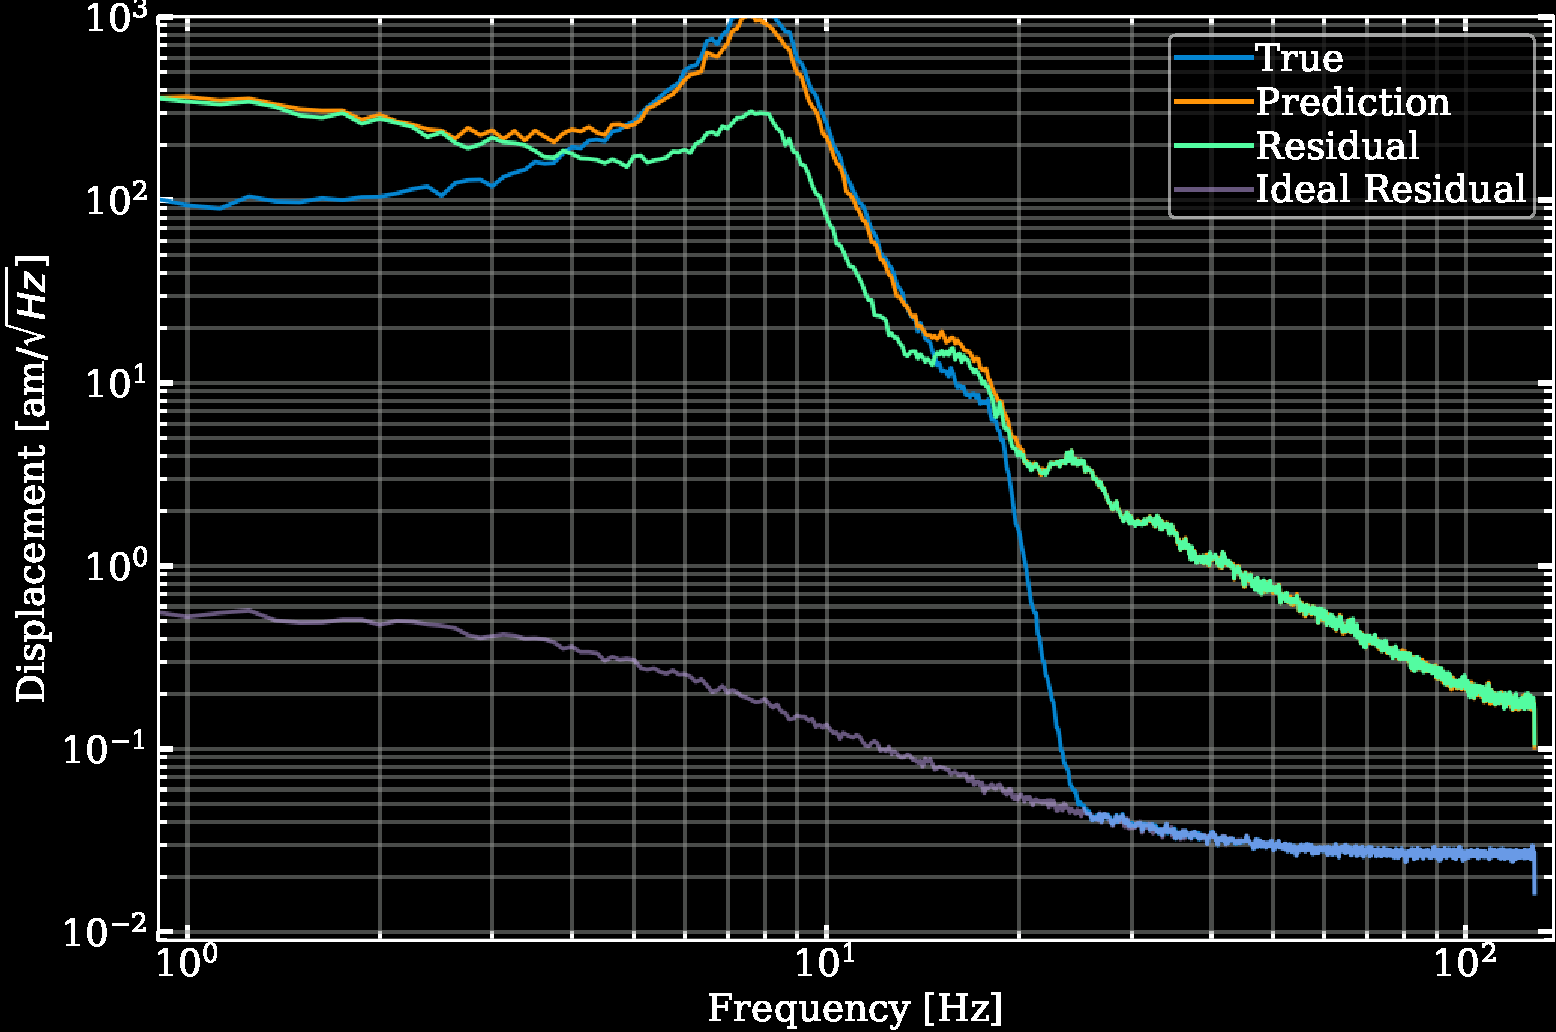
\includegraphics[width=.7\columnwidth]{chapter_noise_sub/etc/spectra16C}
     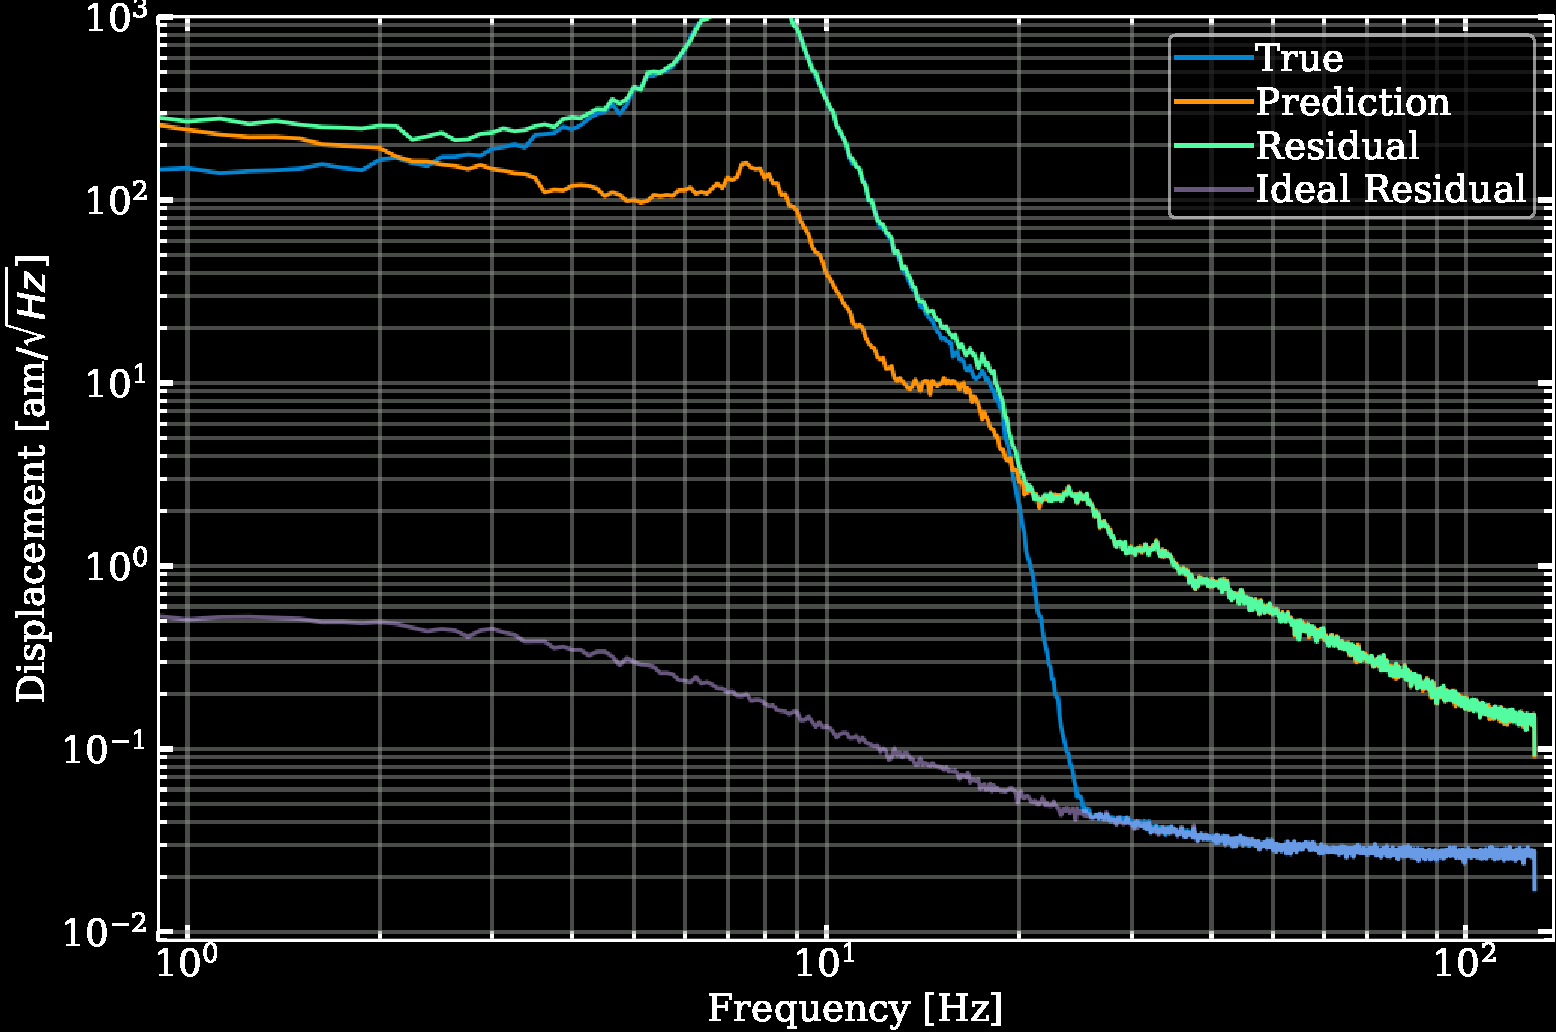
\includegraphics[width=.7\columnwidth]{chapter_noise_sub/etc/spectra32C}
   \caption{Amplitude Spectral densities illustrating subtraction for the colored bilinear mock data with 2 (top panel), 4 (middle panel), and 8 (bottom panel) pairs. Between 10 and 20 Hz, we achieve roughly a factor of 10 reduction between the target/neural network prediction and the residual between the target and prediction}
   \label{fig:ASD2}
\end{figure}

%\begin{figure}[htbp]
%   \centering
%   \subfigure{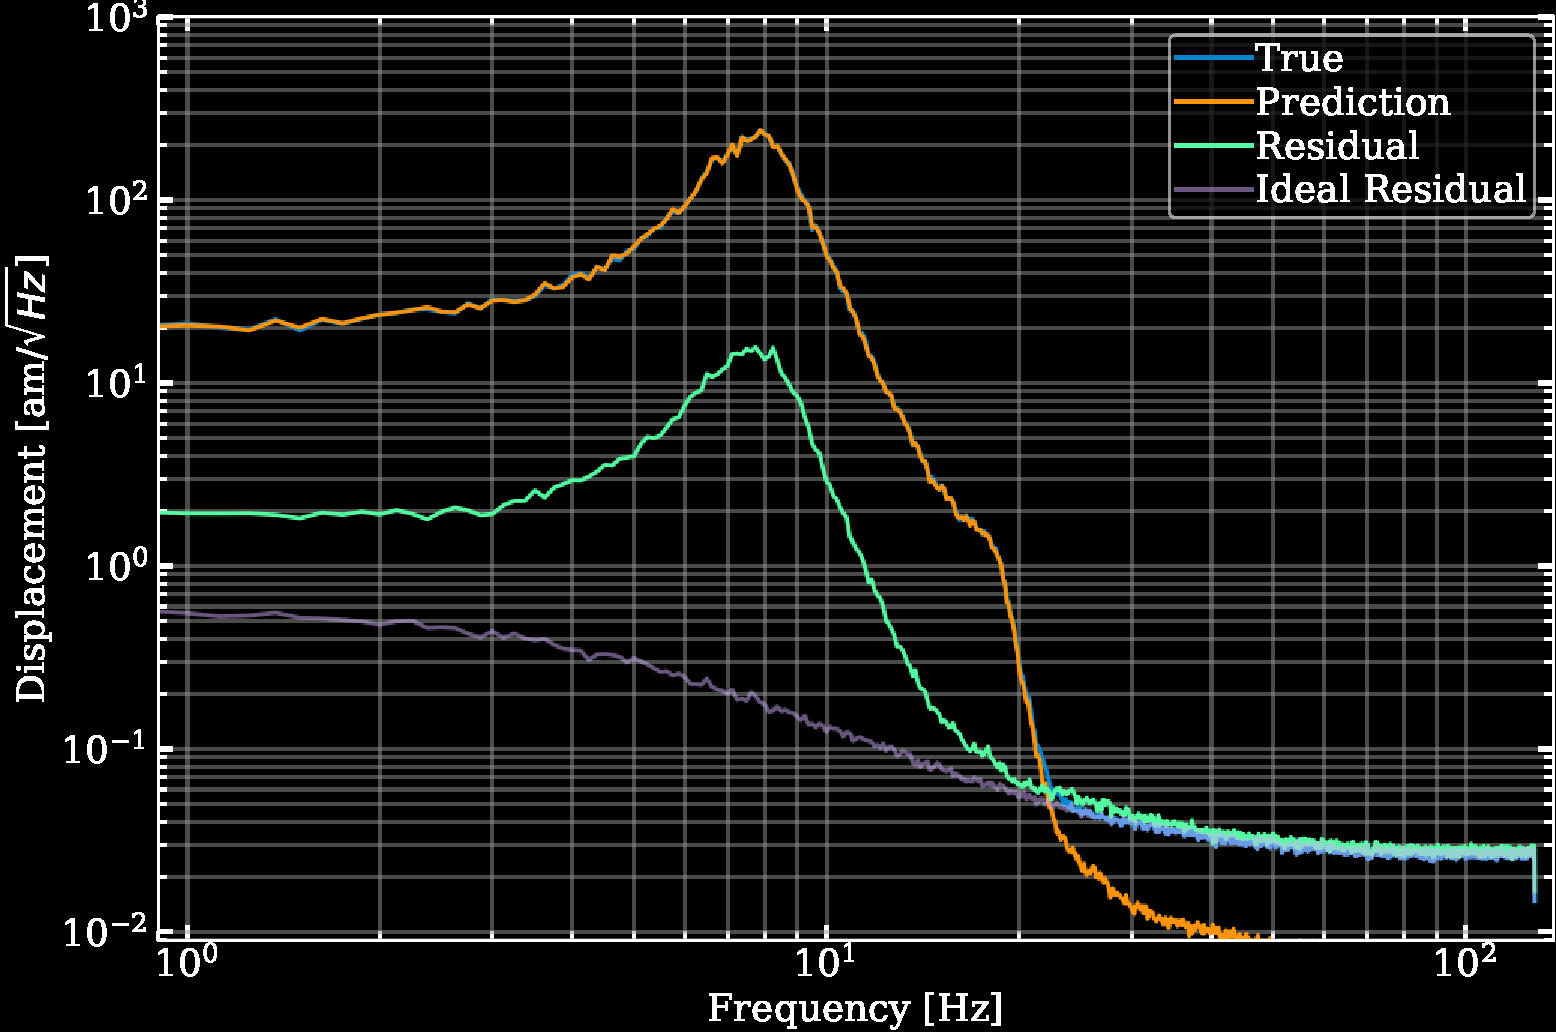
\includegraphics[width=.7\columnwidth]{chapter_noise_sub/etc/spectra1C}}\quad
%   \subfigure{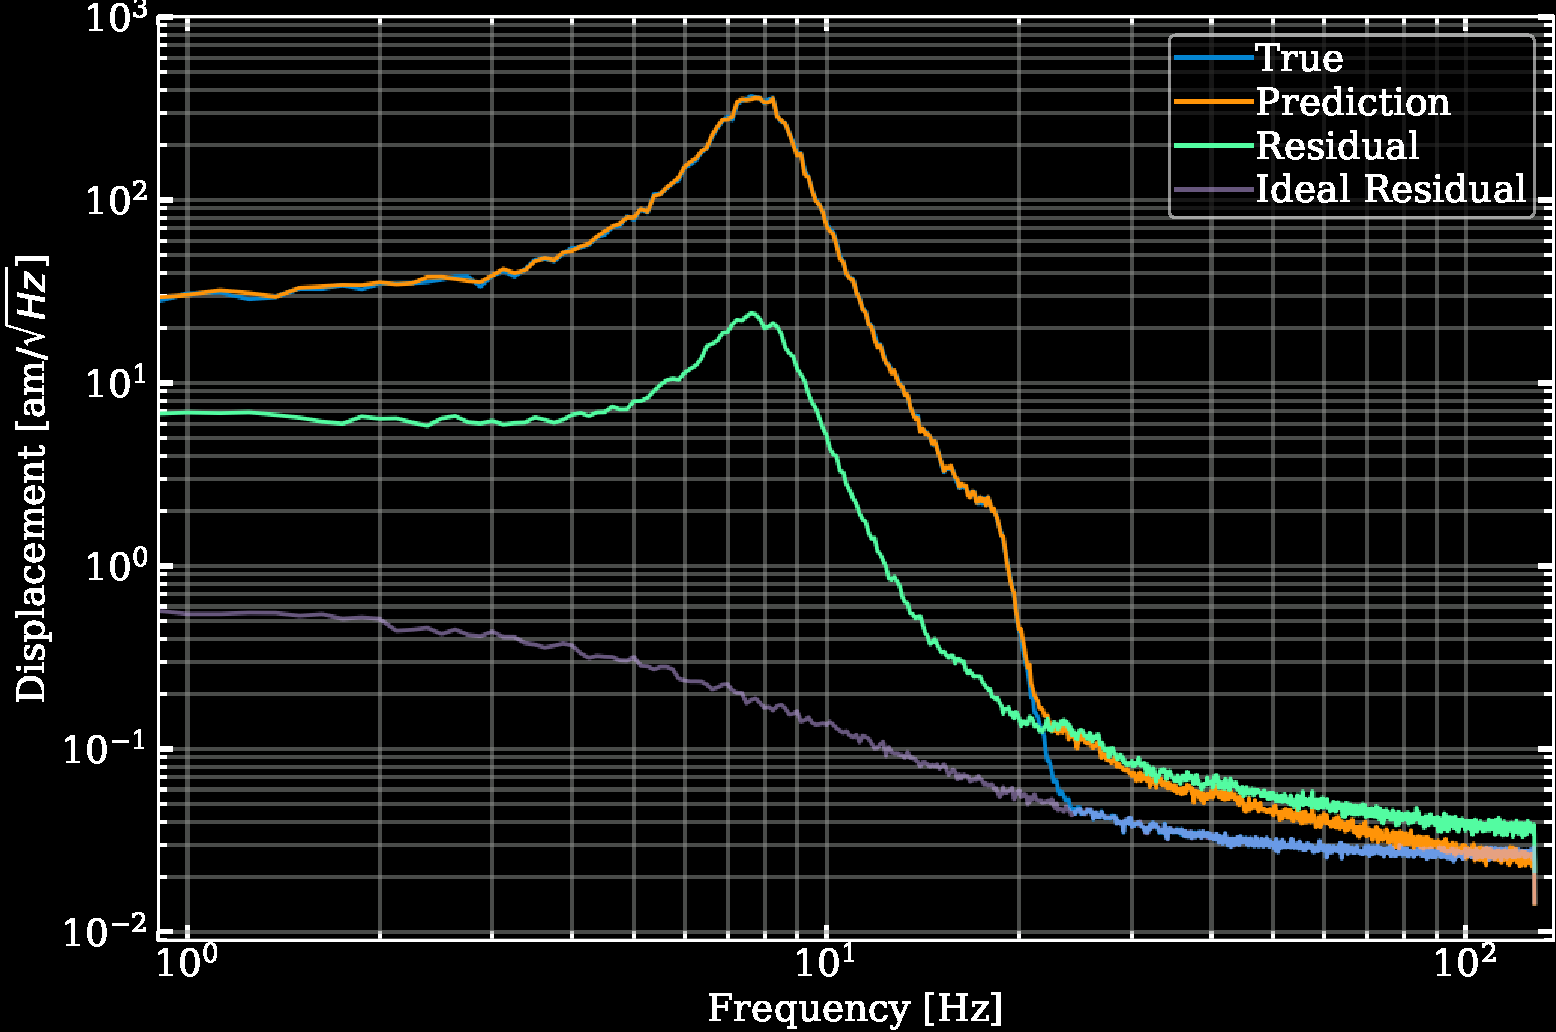
\includegraphics[width=.7\columnwidth]{chapter_noise_sub/etc/spectra2C}}
%   \subfigure{ 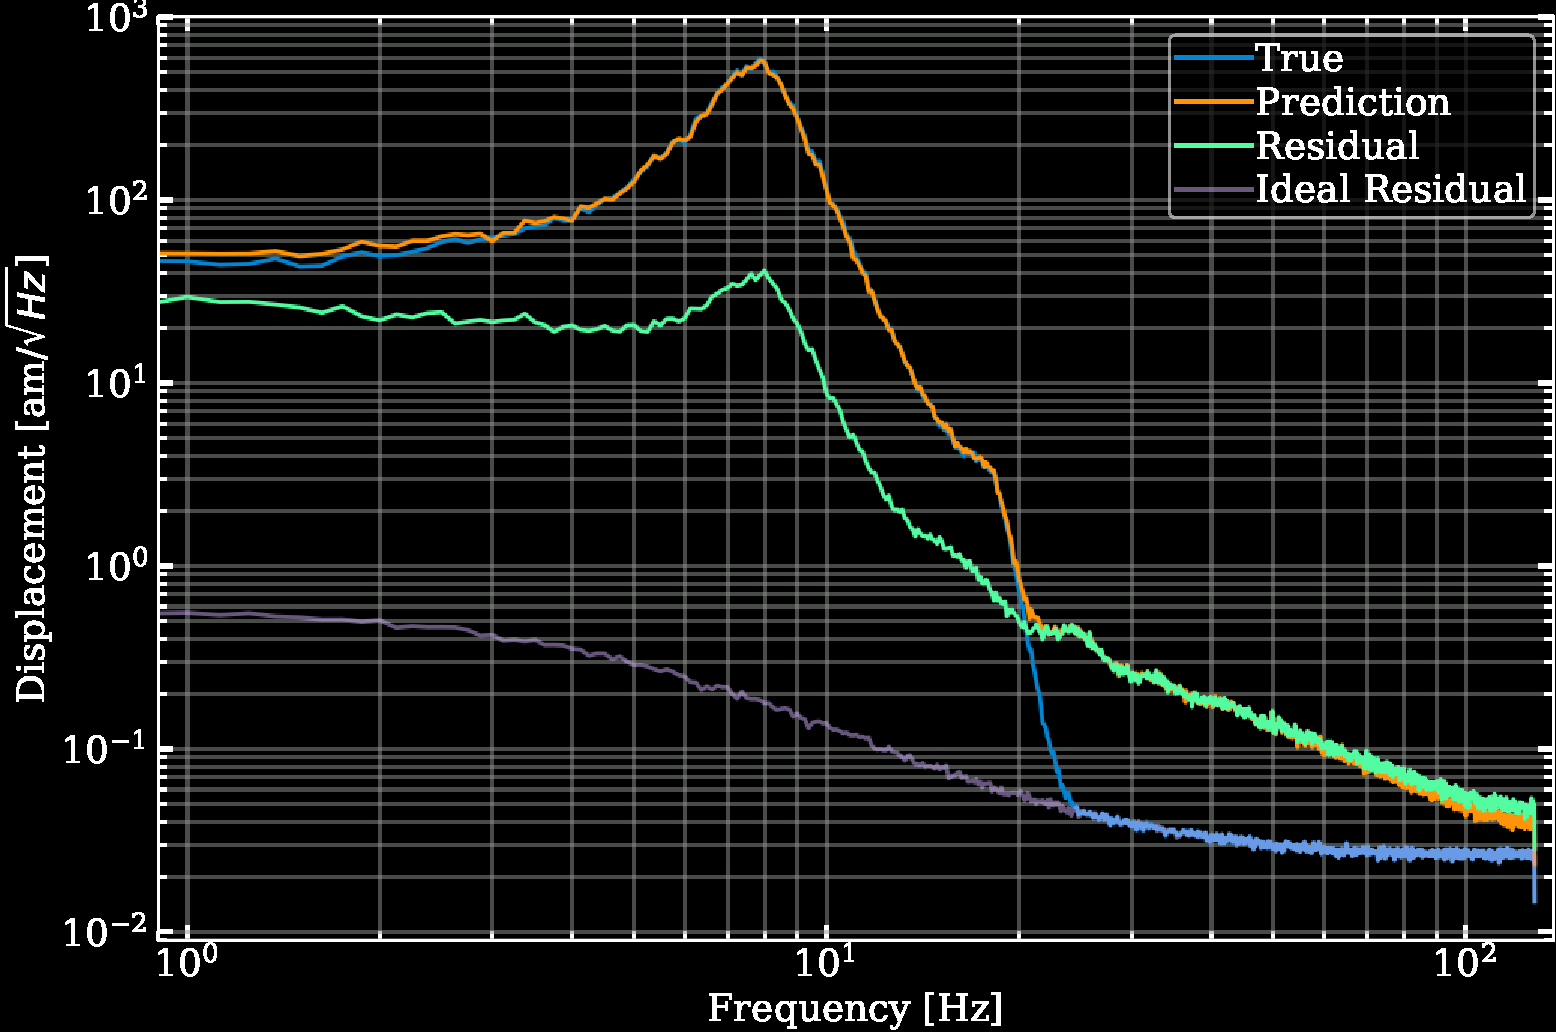
\includegraphics[width=.7\columnwidth]{chapter_noise_sub/etc/spectra4C}}\quad
%   \subfigure{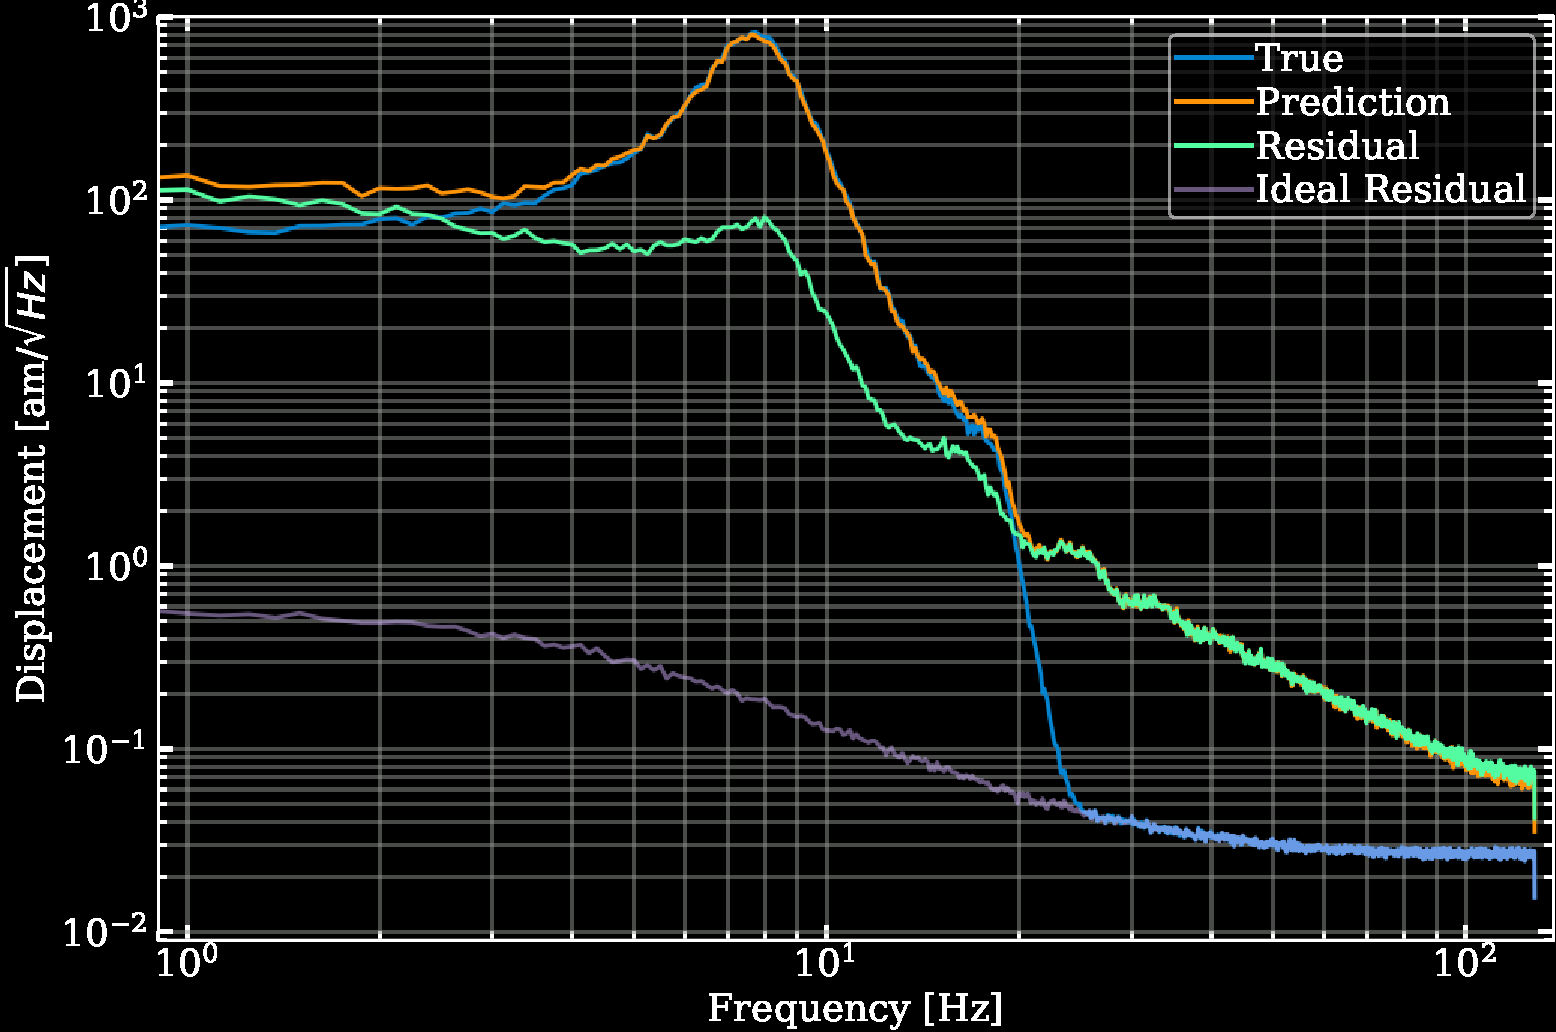
\includegraphics[width=.7\columnwidth]{chapter_noise_sub/etc/spectra8C}}
%   \subfigure{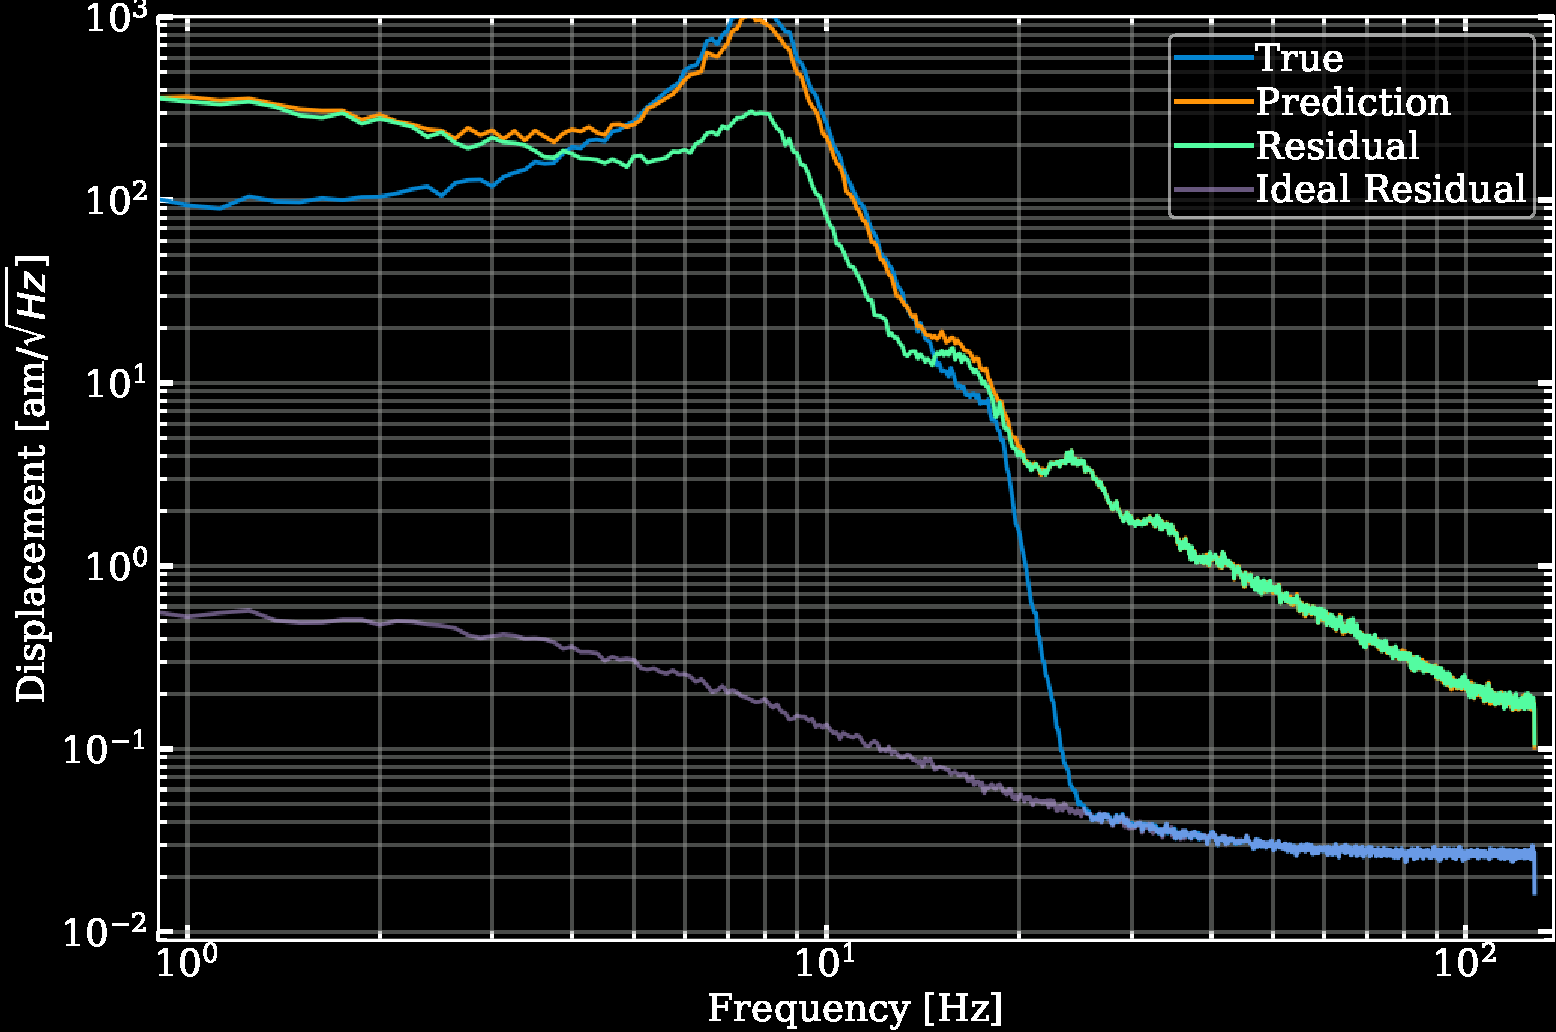
\includegraphics[width=.7\columnwidth]{chapter_noise_sub/etc/spectra16C}}\quad
%   \subfigure{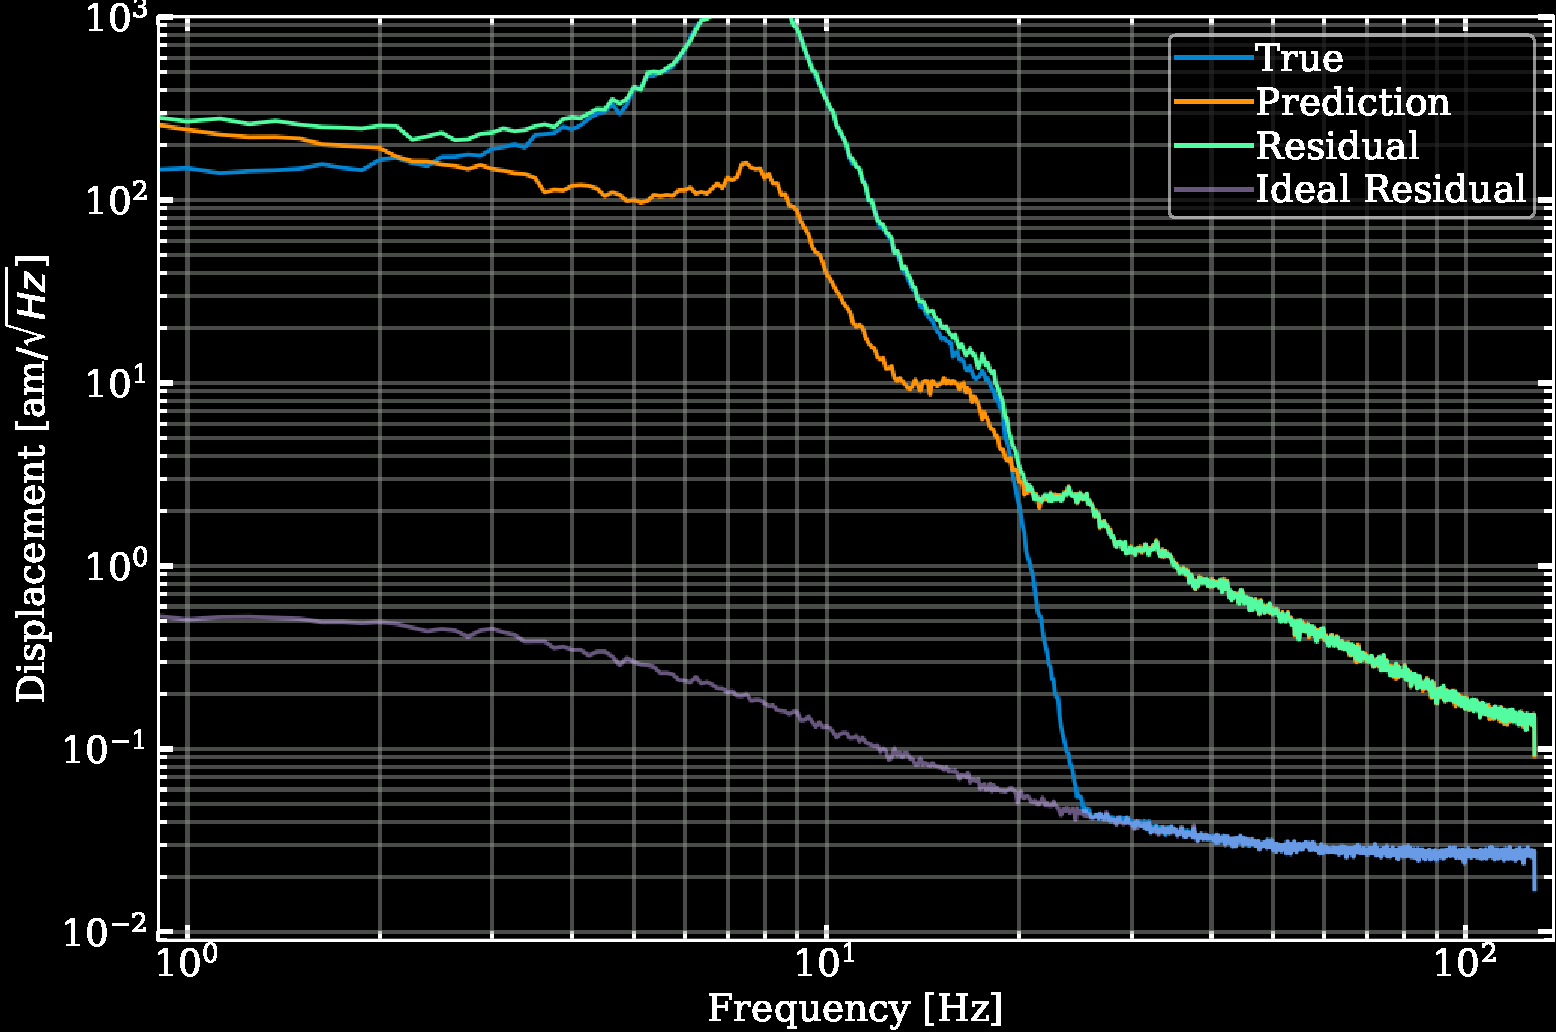
\includegraphics[width=.7\columnwidth]{chapter_noise_sub/etc/spectra32C}}
%   \caption{Amplitude Spectral densities illustrating subtraction for the colored bilinear mock data with 2 (top panel), 4 (middle panel), and 8 (bottom panel) pairs. Between 10 and 20 Hz, we achieve roughly a factor of 10 reduction between the target/neural network prediction and the residual between the target and prediction}
%   \label{fig:ASD1}
%\end{figure}

%\begin{figure}[htbp]
%   \centering
%   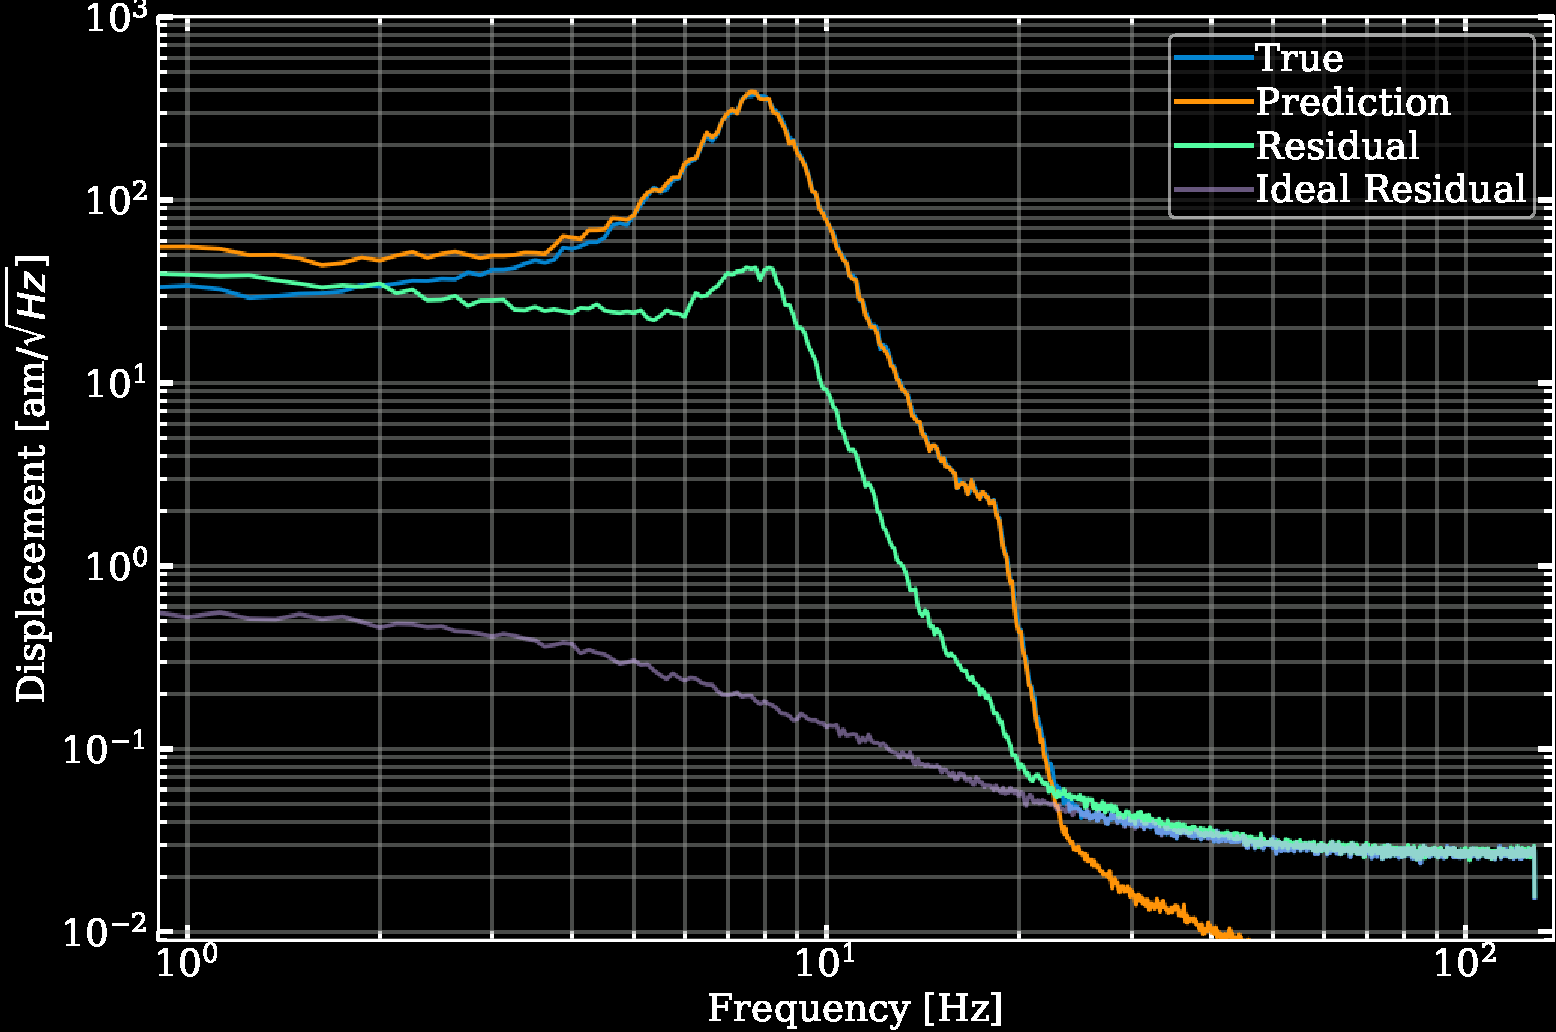
\includegraphics[width=.7\columnwidth]{chapter_noise_sub/etc/spectra2}
%   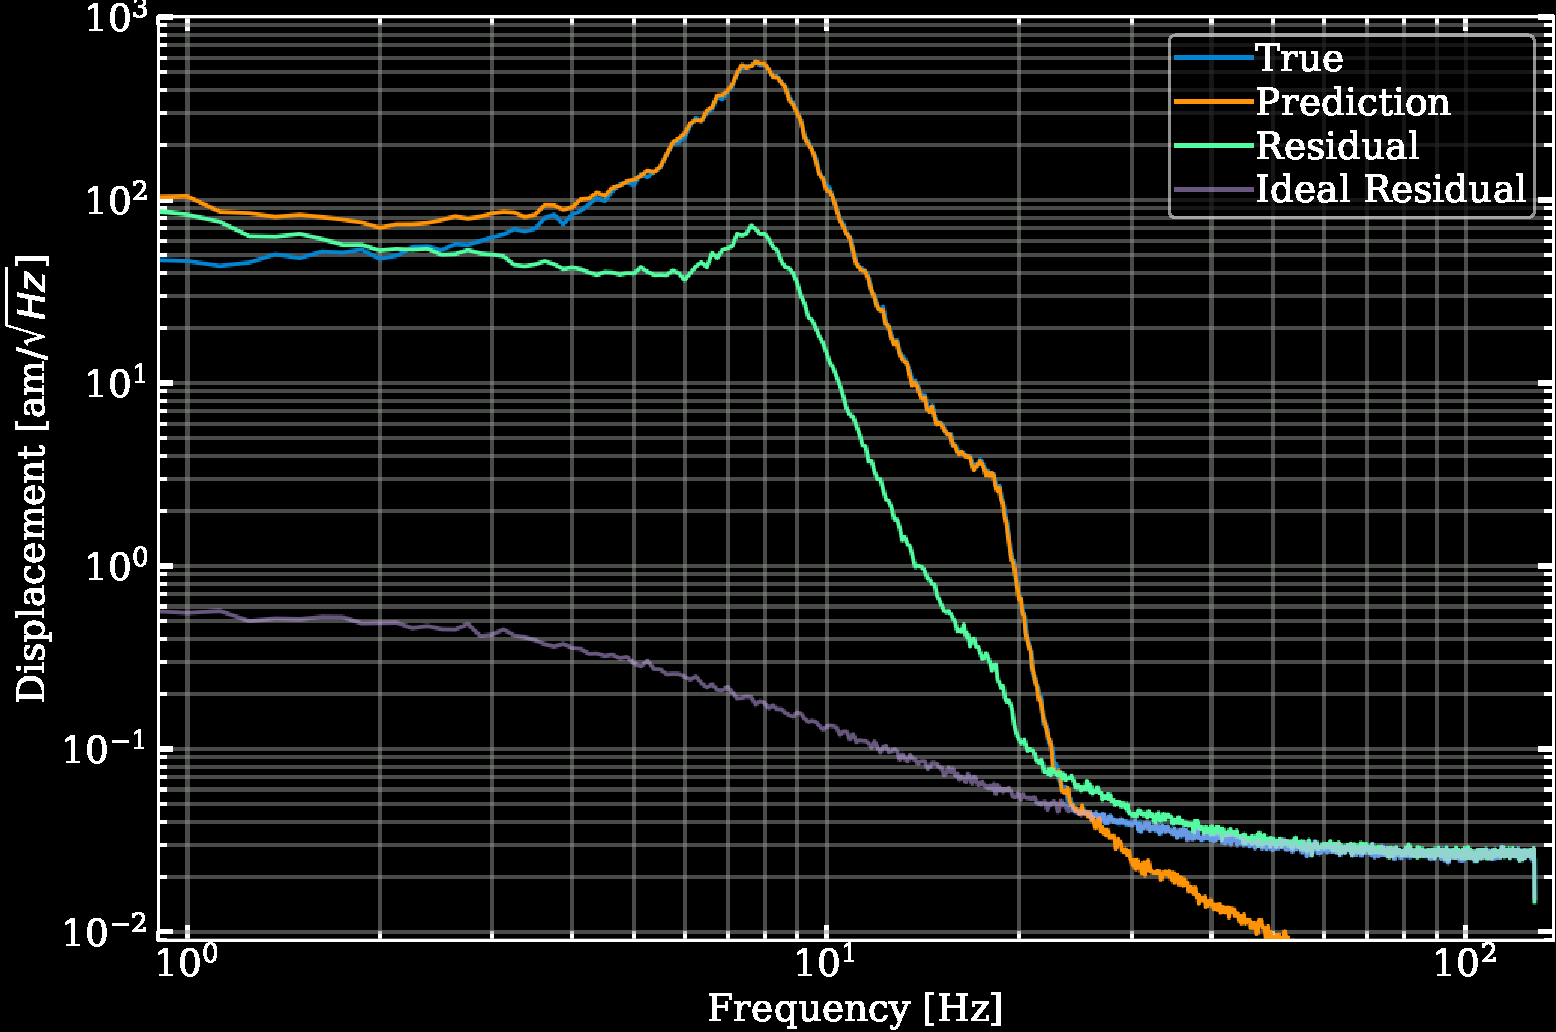
\includegraphics[width=.7\columnwidth]{chapter_noise_sub/etc/spectra4}
%   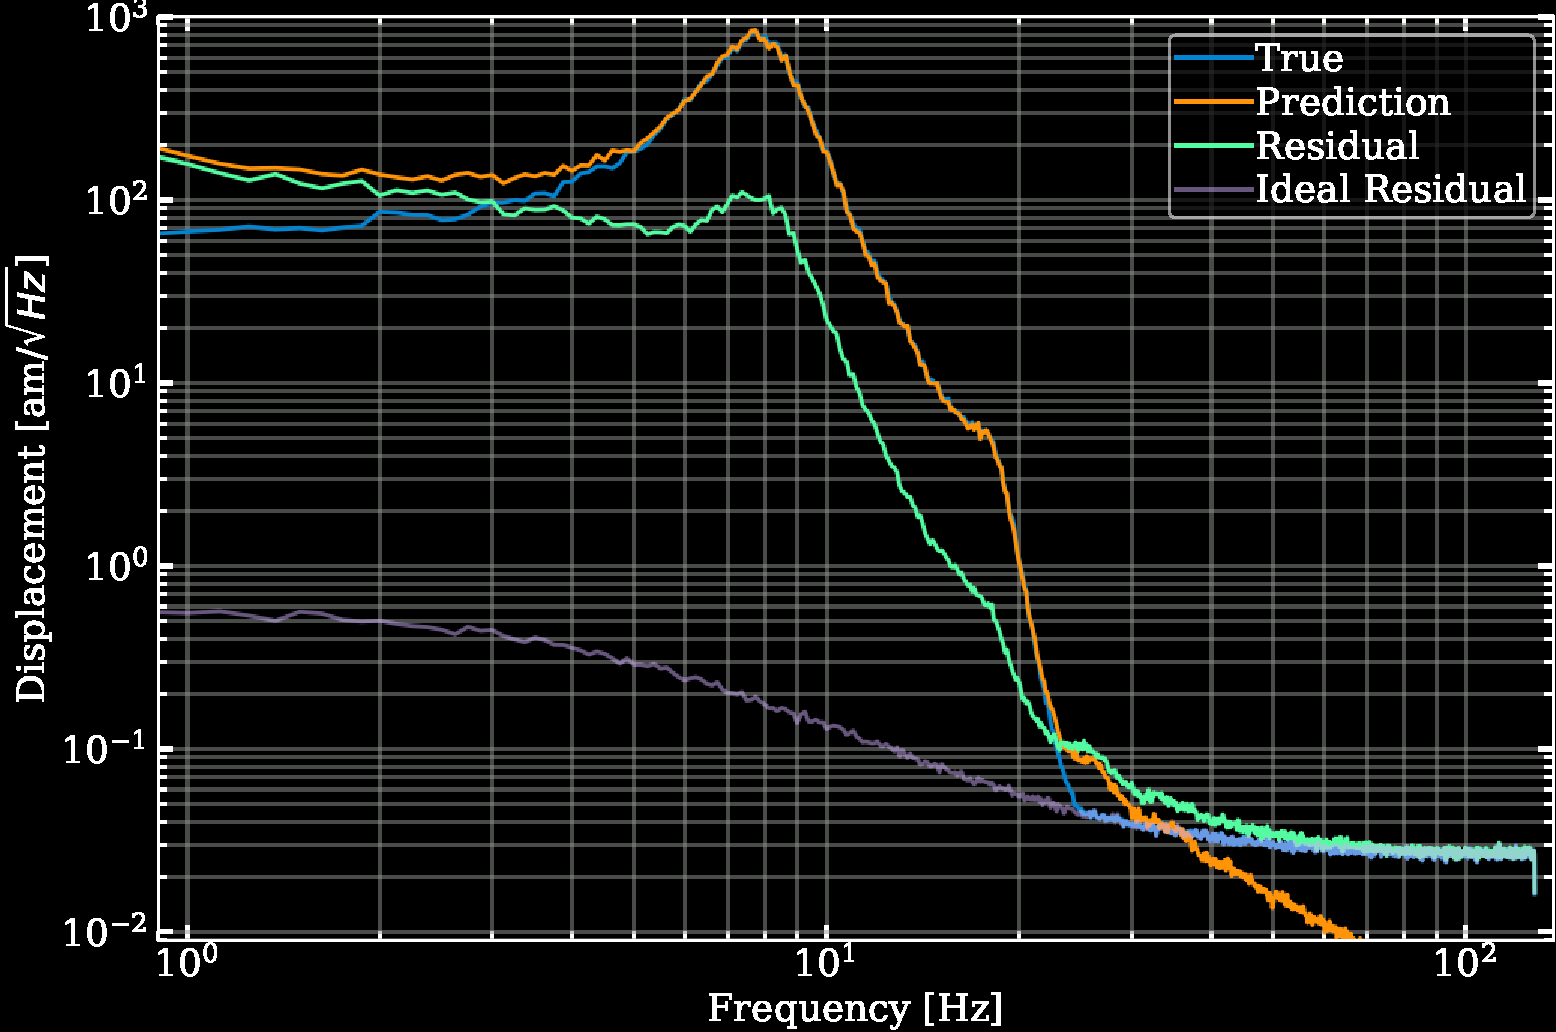
\includegraphics[width=.7\columnwidth]{chapter_noise_sub/etc/spectra8}
%   \caption{Amplitude Spectral densities illustrating subtraction for the colored bilinear mock data with 2 (top panel), 4 (middle panel), and 8 (bottom panel) pairs. Between 10 and 20 Hz, we achieve roughly a factor of 10 reduction between the target/neural network prediction and the residual between the target and prediction}
%   \label{fig:ASD1}
%\end{figure}

Even if we had the optimal neural network, we wouldn't obtain a perfect subtraction because of measurement noise incorporated in the colored bilinear mock data. In figures \ref{fig:ASD1} and \ref{fig:ASD2}, we also show the ideal subtraction. The ideal prediction is calculated by running the witnesses with the measurement noise through the bilinear coupling function. We are actively investigating why our network is off by two orders of magnitude from the ideal subtraction.

%\begin{figure}[htbp]
%   \centering
%   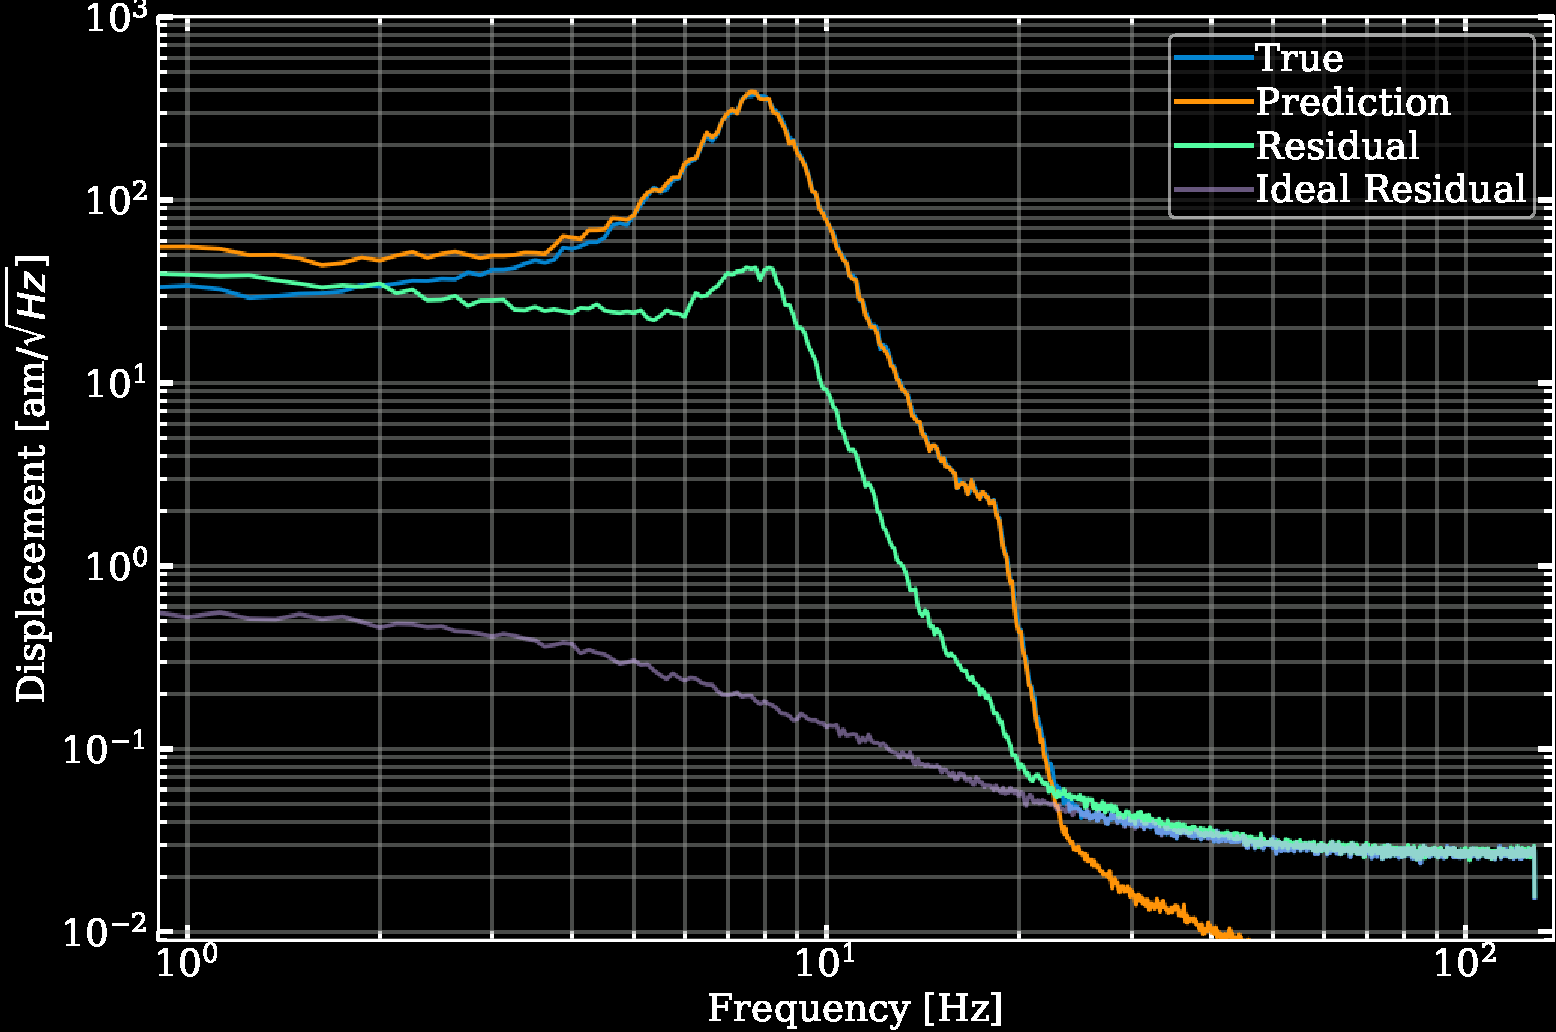
\includegraphics[width=.7\columnwidth]{chapter_noise_sub/etc/spectra2}
%   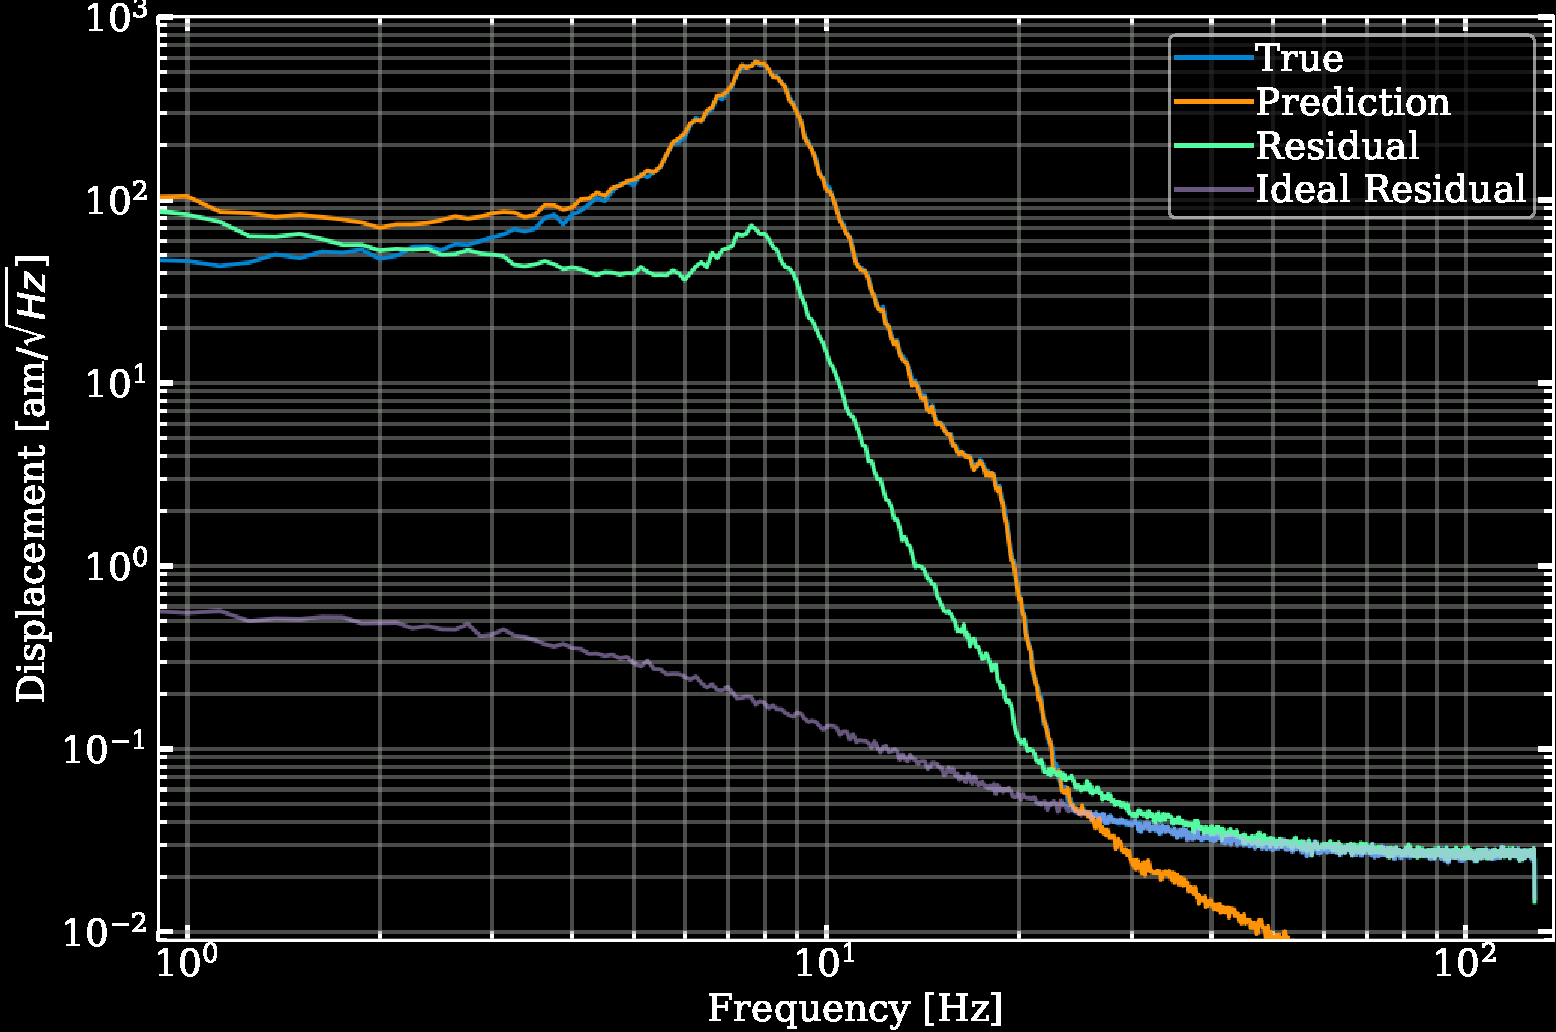
\includegraphics[width=.7\columnwidth]{chapter_noise_sub/etc/spectra4}
%   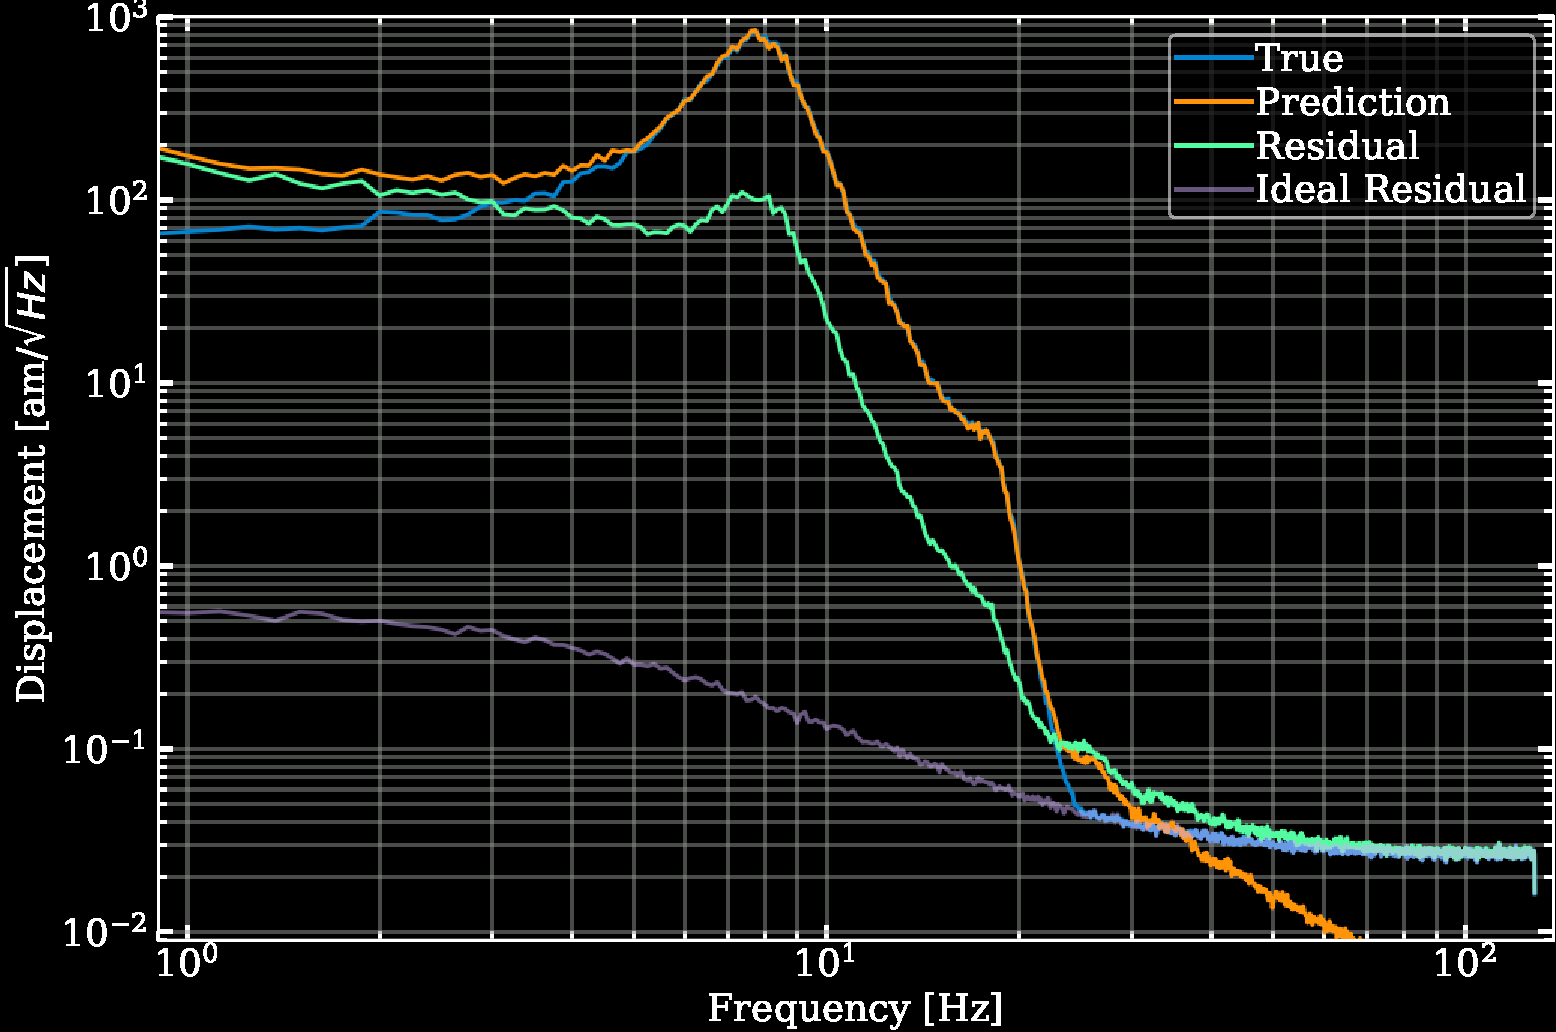
\includegraphics[width=.7\columnwidth]{chapter_noise_sub/etc/spectra8}
%   \caption{Amplitude Spectral densities illustrating subtraction for the colored bilinear mock data with 2 (top panel), 4 (middle panel), and 8 (bottom panel) pairs. Between 10 and 20 Hz, we achieve roughly a factor of 10 reduction between the target/neural network prediction and the residual between the target and prediction}
%   \label{fig:ASD1}
%\end{figure}

%\begin{figure}[htbp]
%\centering
%	\begin{subfigure}[t]{0.45\textwidth}
%   		\centering
%   		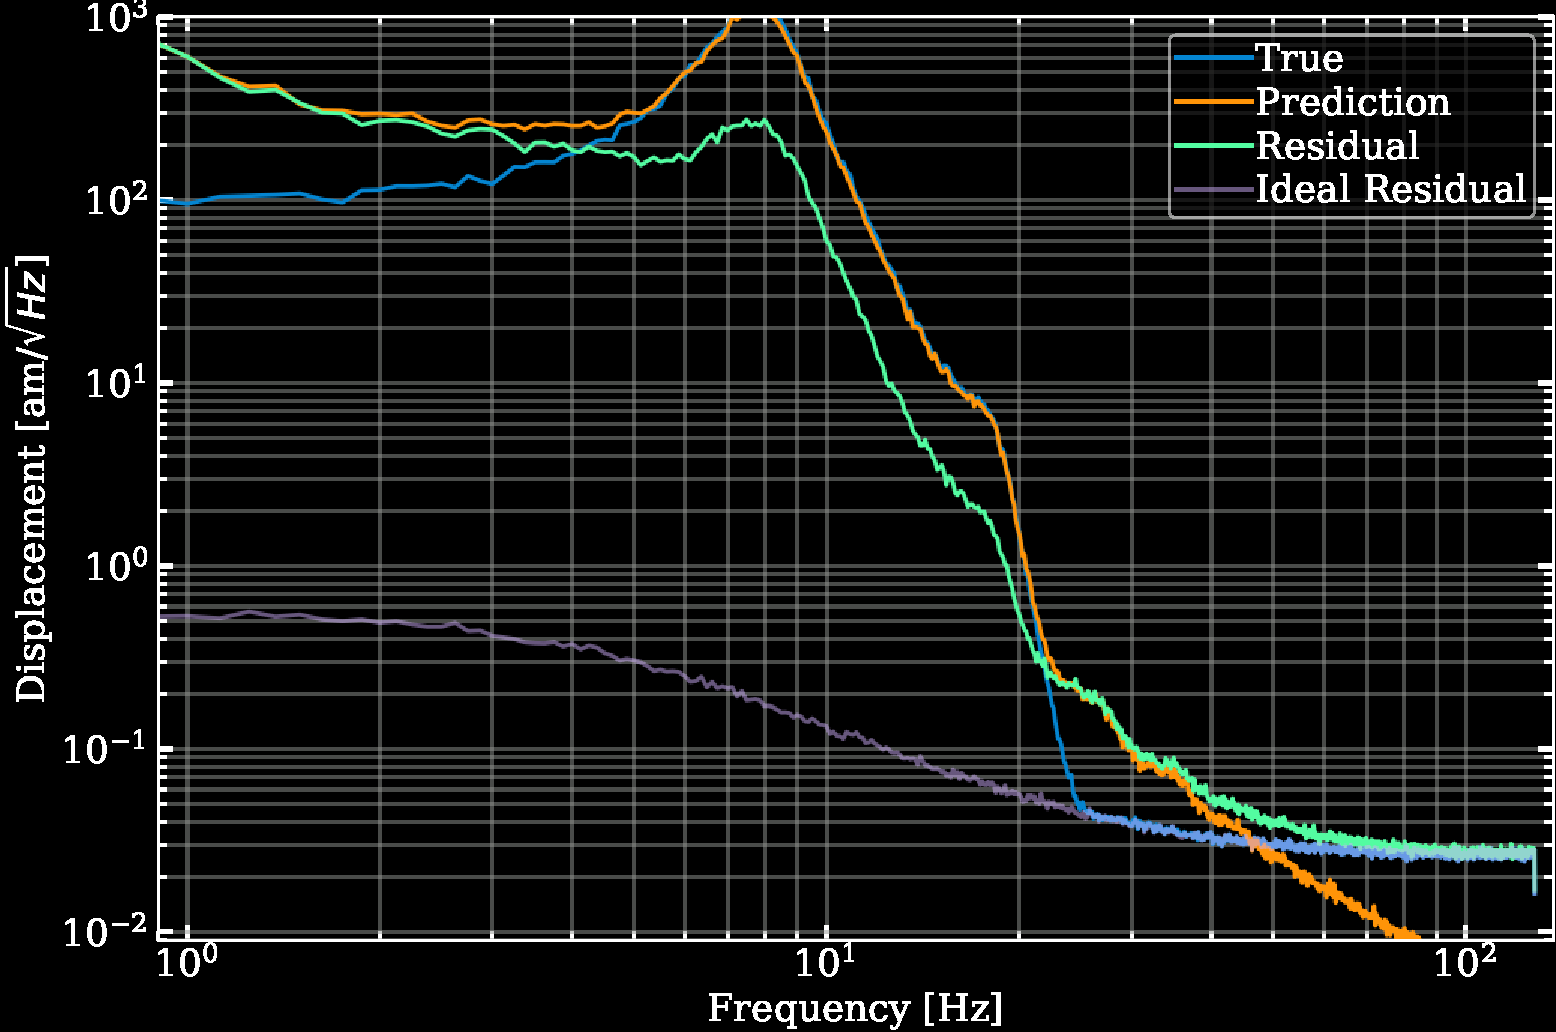
\includegraphics[width=1.3\linewidth]{chapter_noise_sub/etc/spectra16}
%		\caption{...}  \label{fig:ASD2-A}
%	\end{subfigure}
%	\hfill
%	\begin{subfigure}[t]{0.45\textwidth}
%		\centering
%		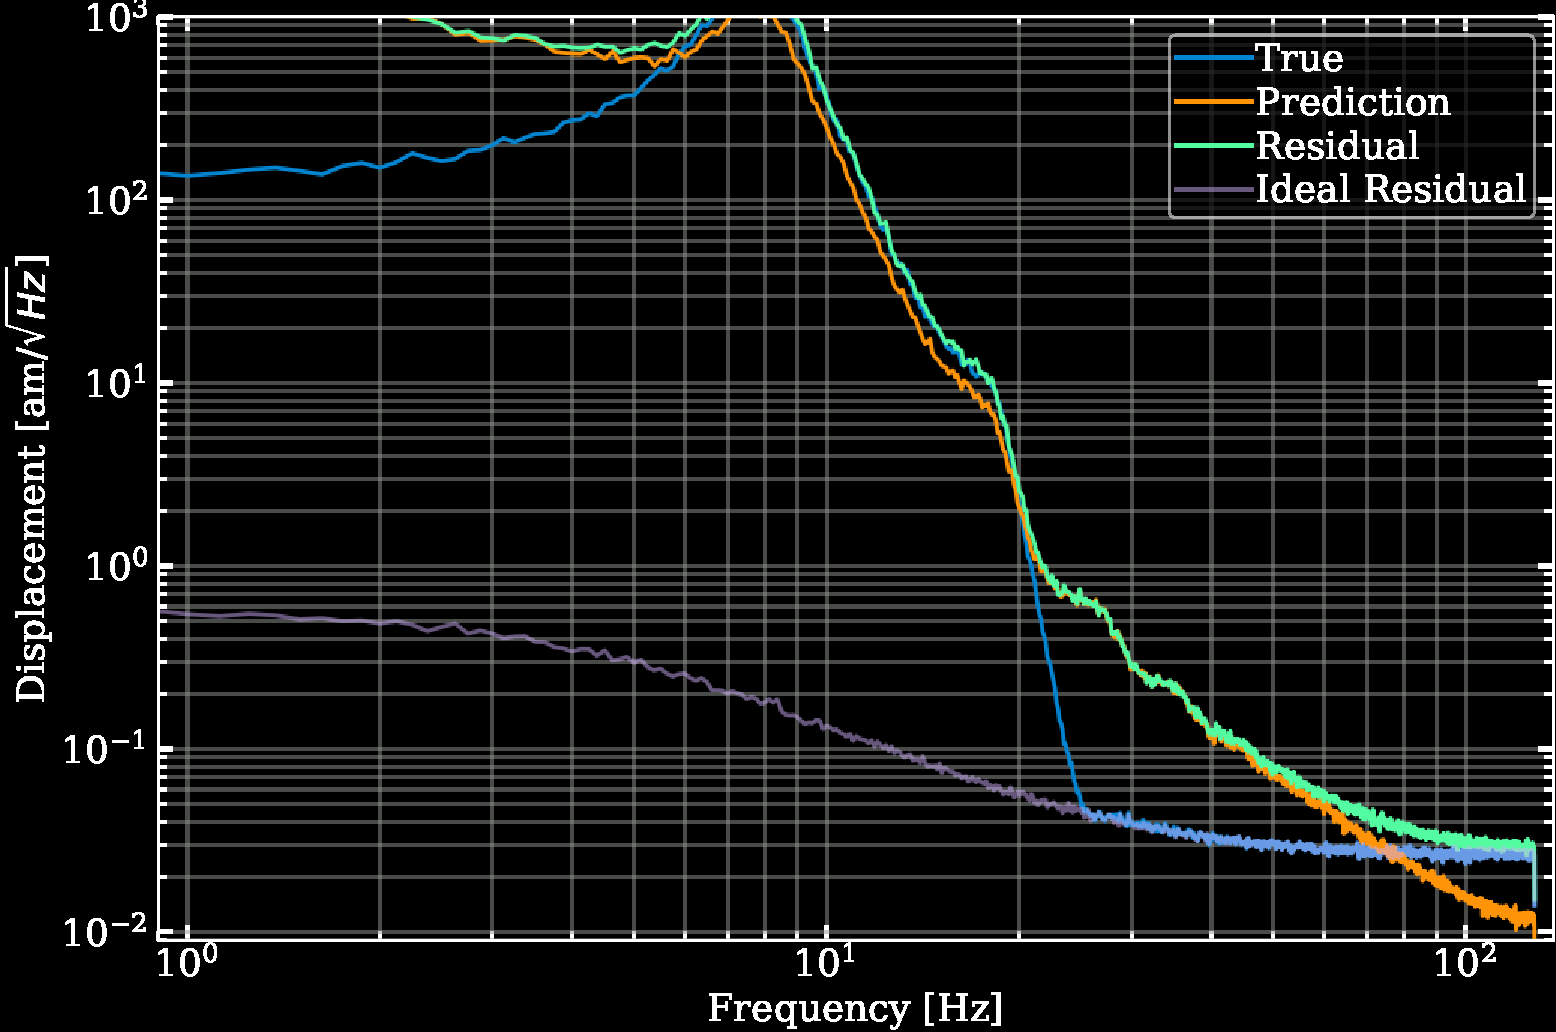
\includegraphics[width=1.3\linewidth]{chapter_noise_sub/etc/spectra32}
%  		 \caption{...} \label{fig:ASD2-B}
% 	\end{subfigure}
%	\caption{...}
%\end{figure}

%\begin{figure}[htbp]
%   \centering
%   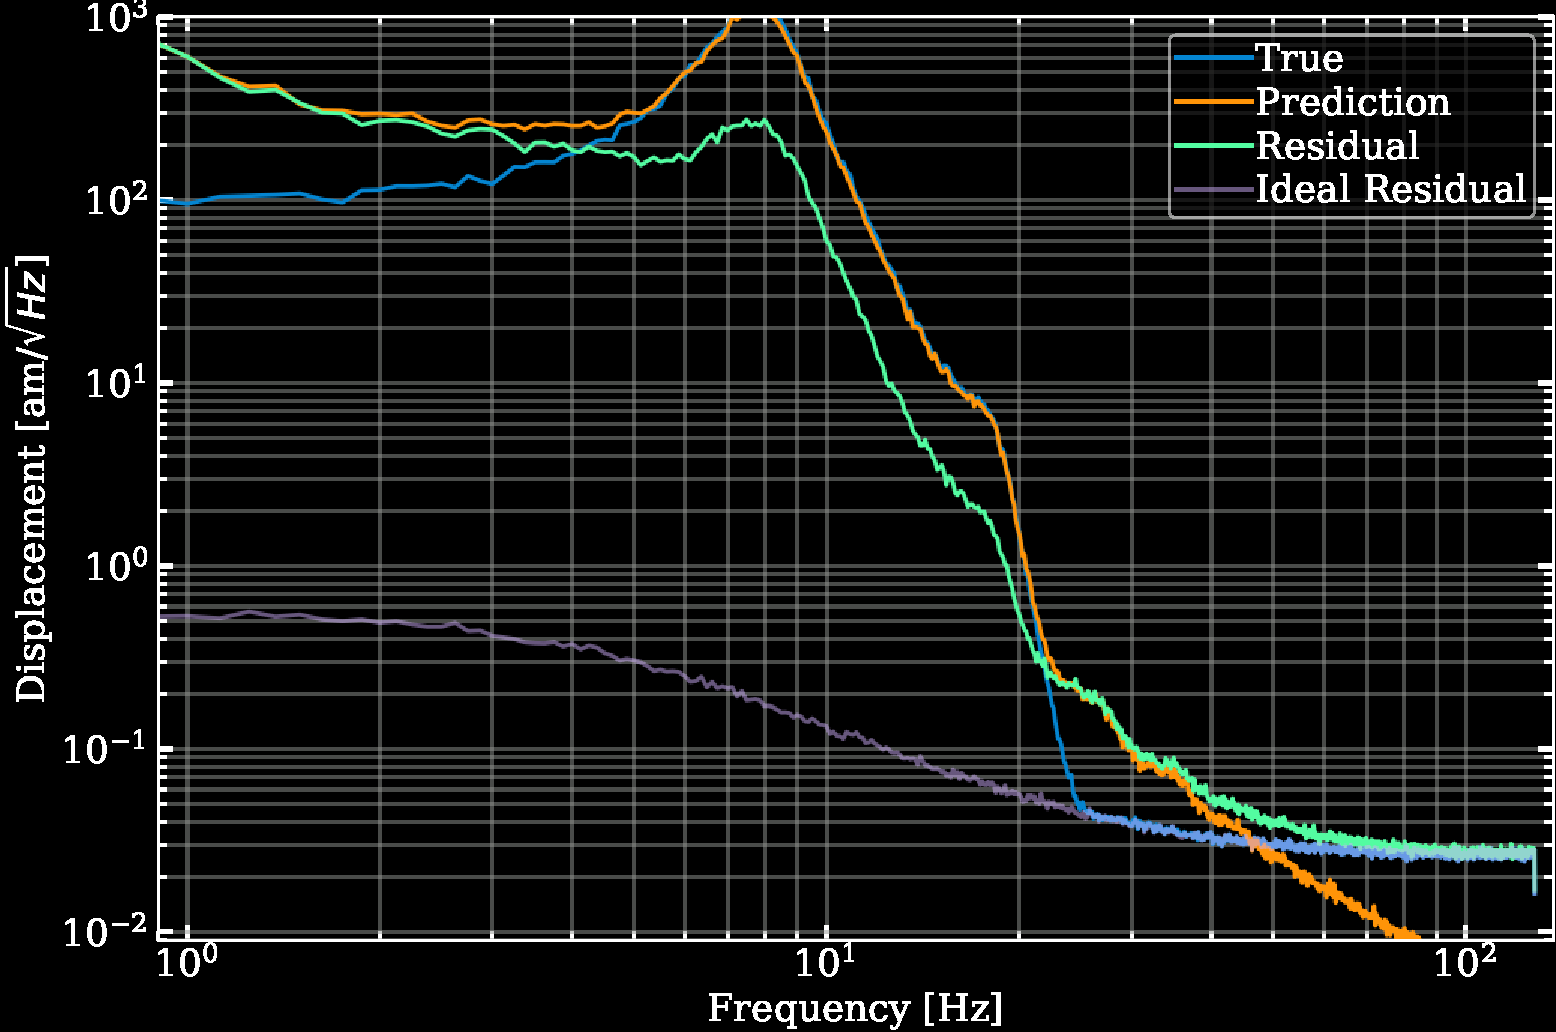
\includegraphics[width=.7\columnwidth]{chapter_noise_sub/etc/spectra16}
%   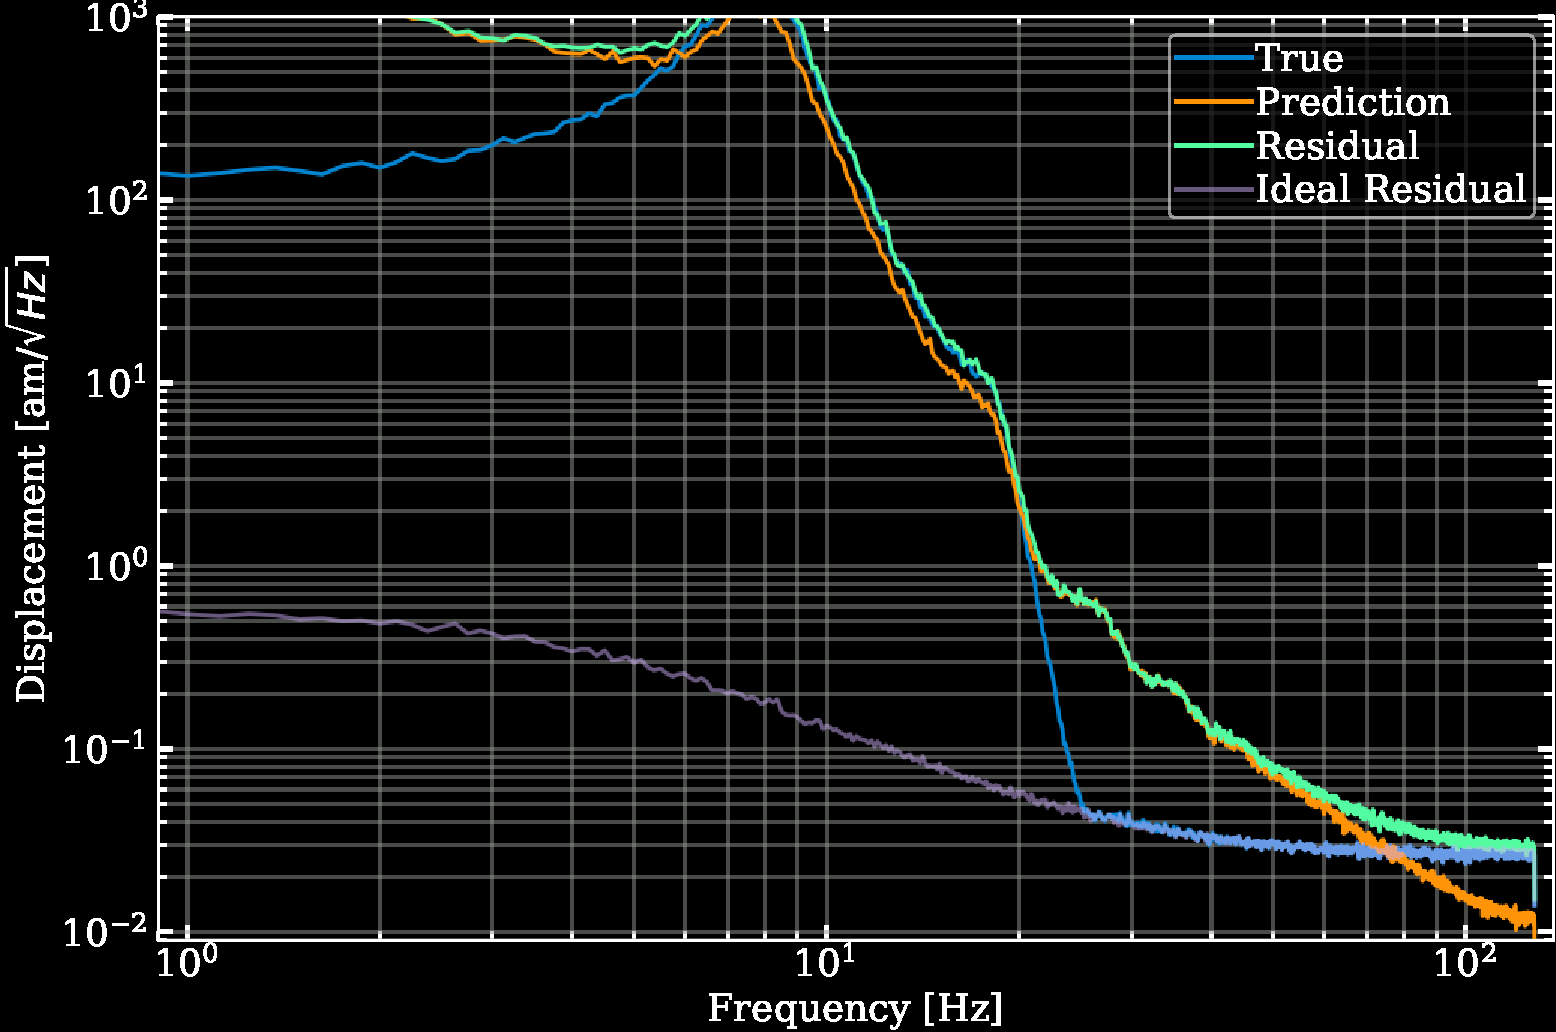
\includegraphics[width=.7\columnwidth]{chapter_noise_sub/etc/spectra32}
%   \caption{Amplitude Spectral densities illustrating subtraction for the colored bilinear mock data with 16 (top panel) and 32 (bottom panel) pairs. For 16 pairs, between 10 and 20 Hz, we achieve roughly a factor of 4 reduction between the target/neural network prediction and the residual between the target and prediction, while we achieve no reduction for 32 pairs. }
%   \label{fig:ASD2}
%\end{figure}

\begin{figure}[htbp]
   \centering
   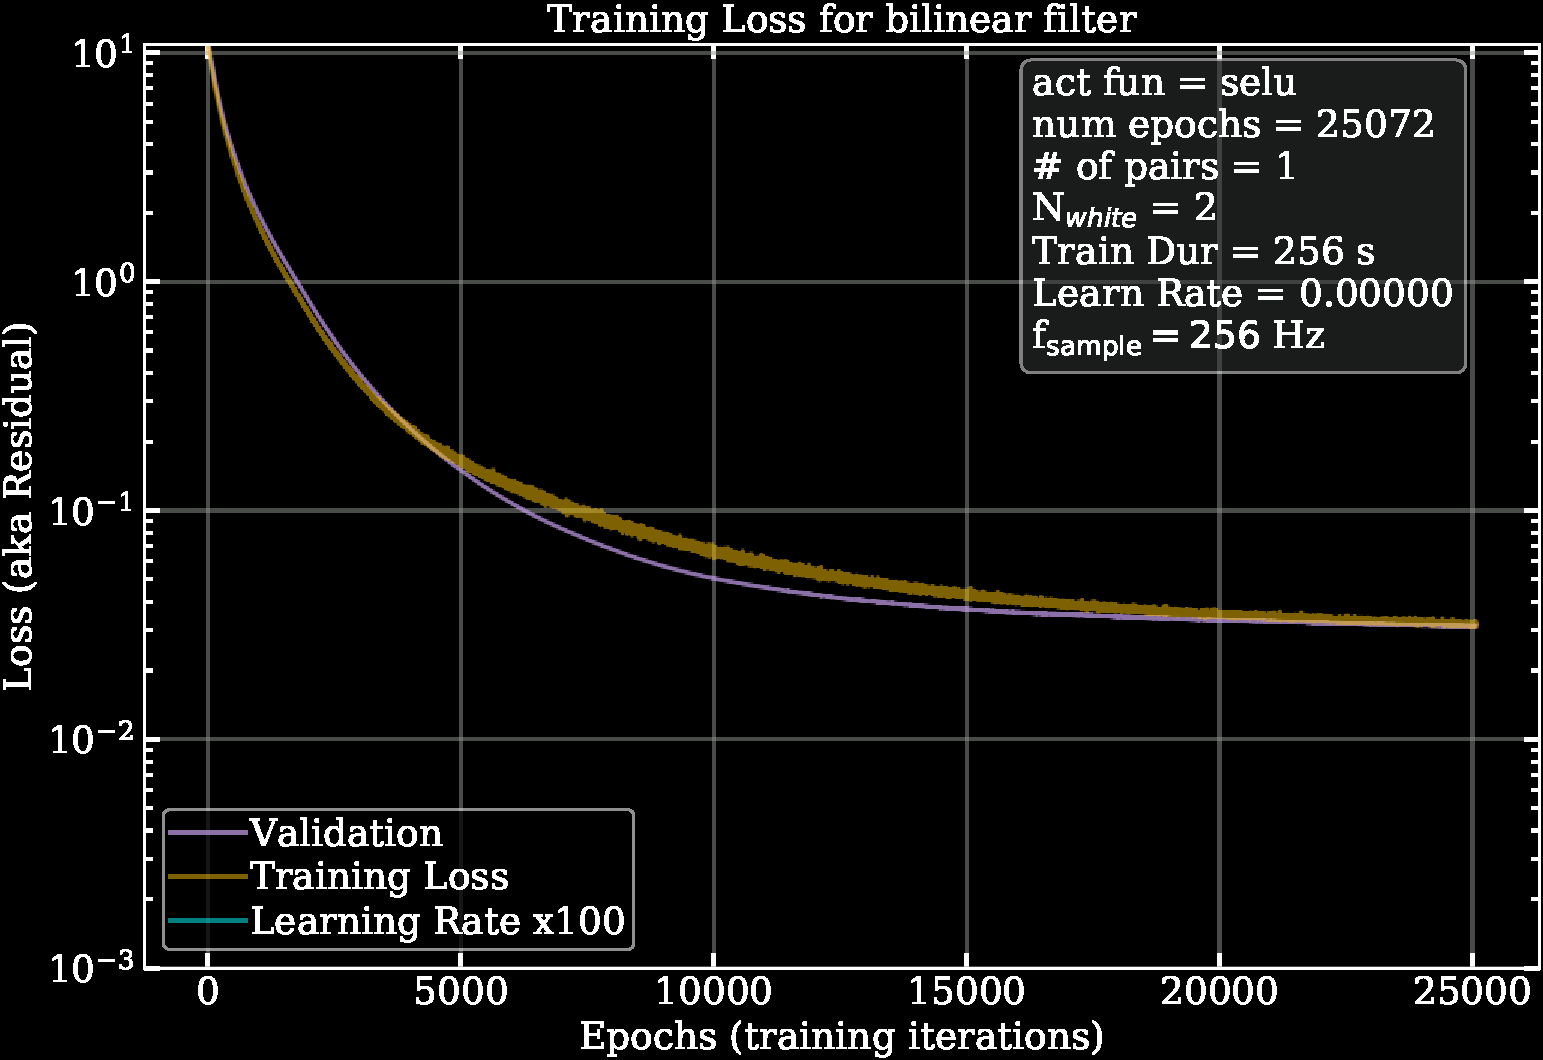
\includegraphics[width=.7\columnwidth]{chapter_noise_sub/etc/loss1C}
   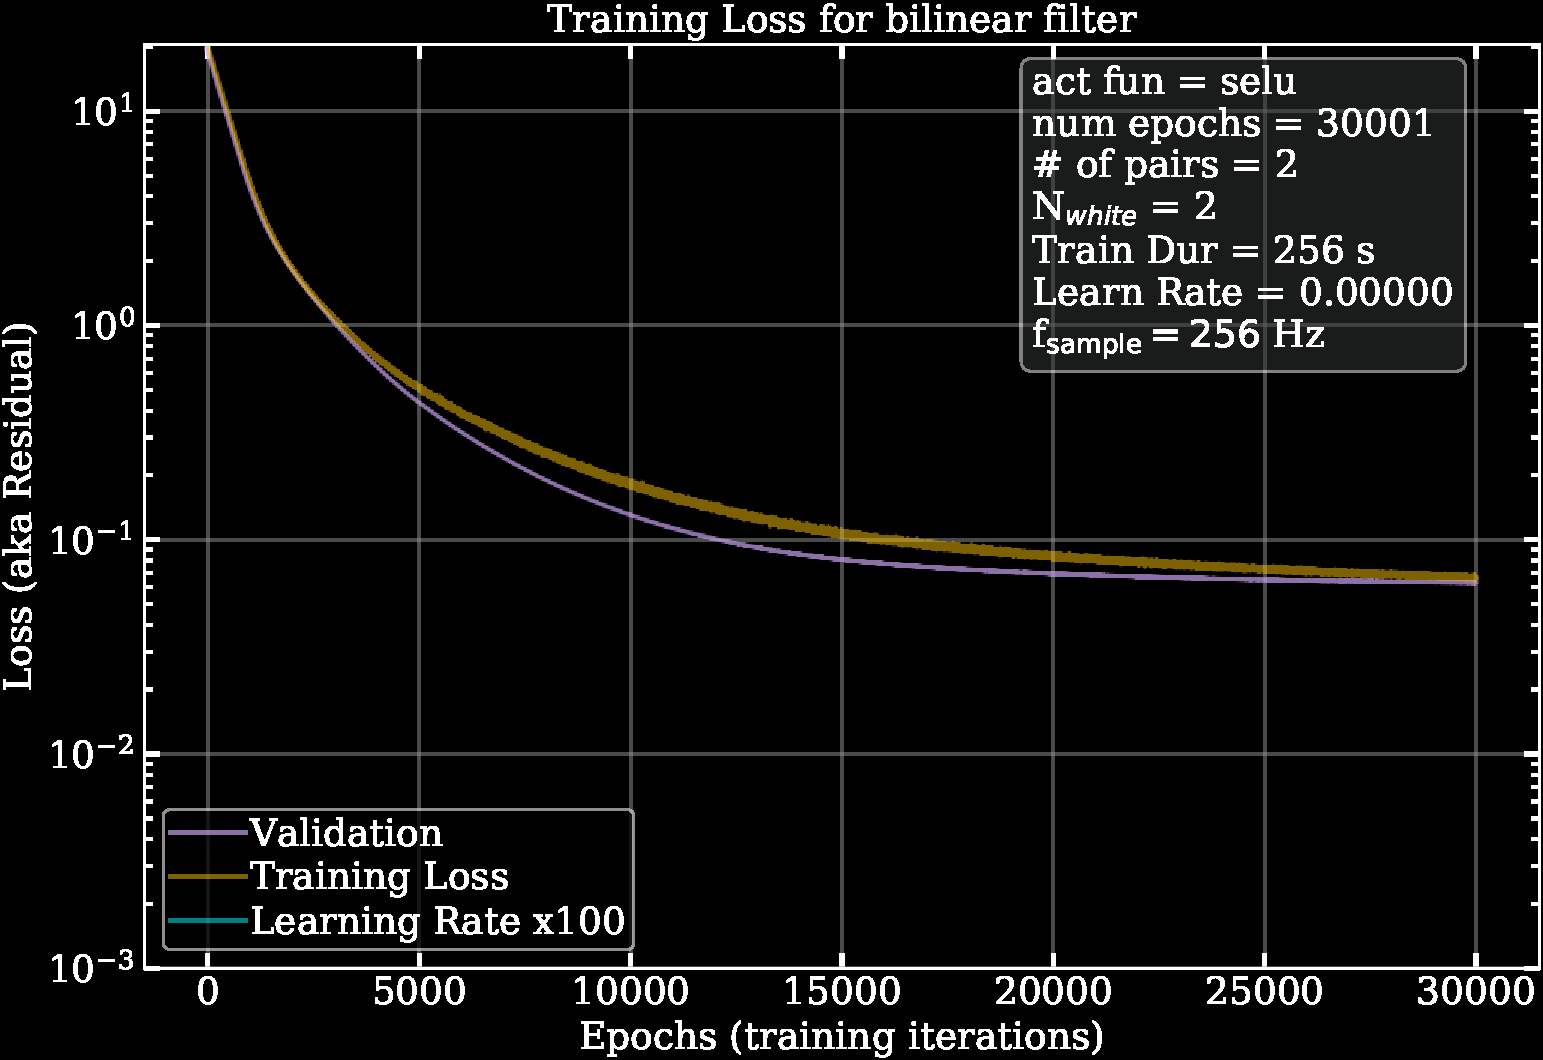
\includegraphics[width=.7\columnwidth]{chapter_noise_sub/etc/loss2C}
   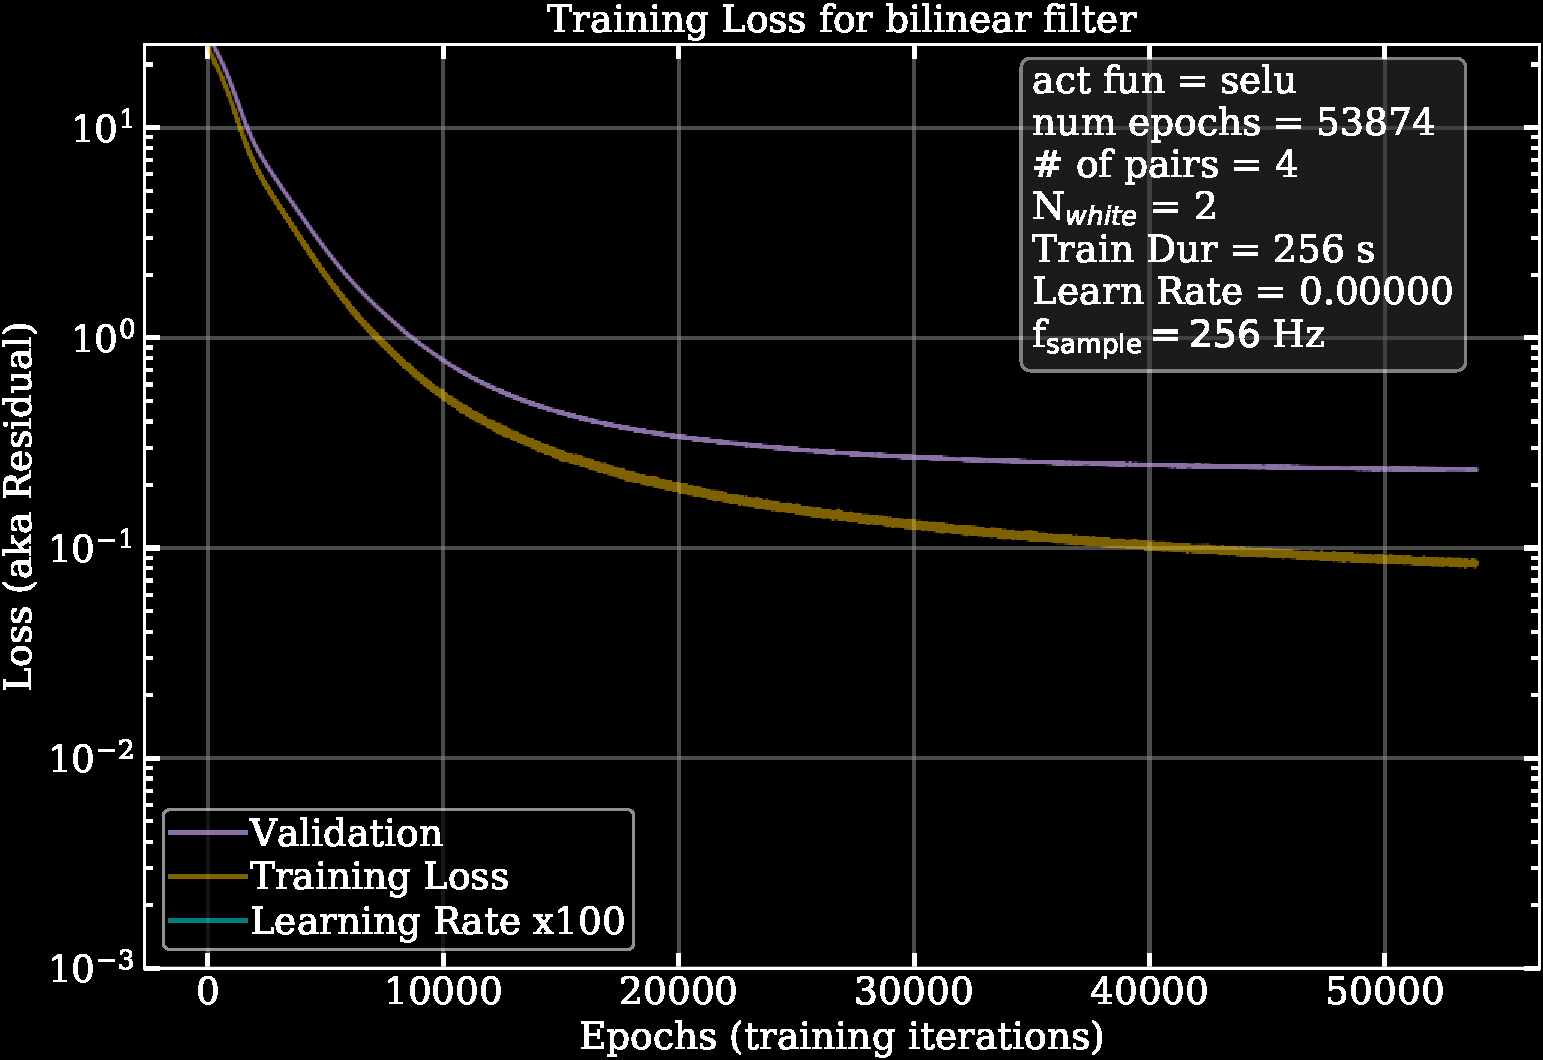
\includegraphics[width=.7\columnwidth]{chapter_noise_sub/etc/loss4C}
   \caption{The loss plotted versus epoch illustrating successful learning for the colored bilinear mock data with 2 (top panel) , 4 (middle panel), and 8 (bottom panel) pairs.}
   \label{fig:loss1}
\end{figure}

\begin{figure}[htbp]
   \centering
   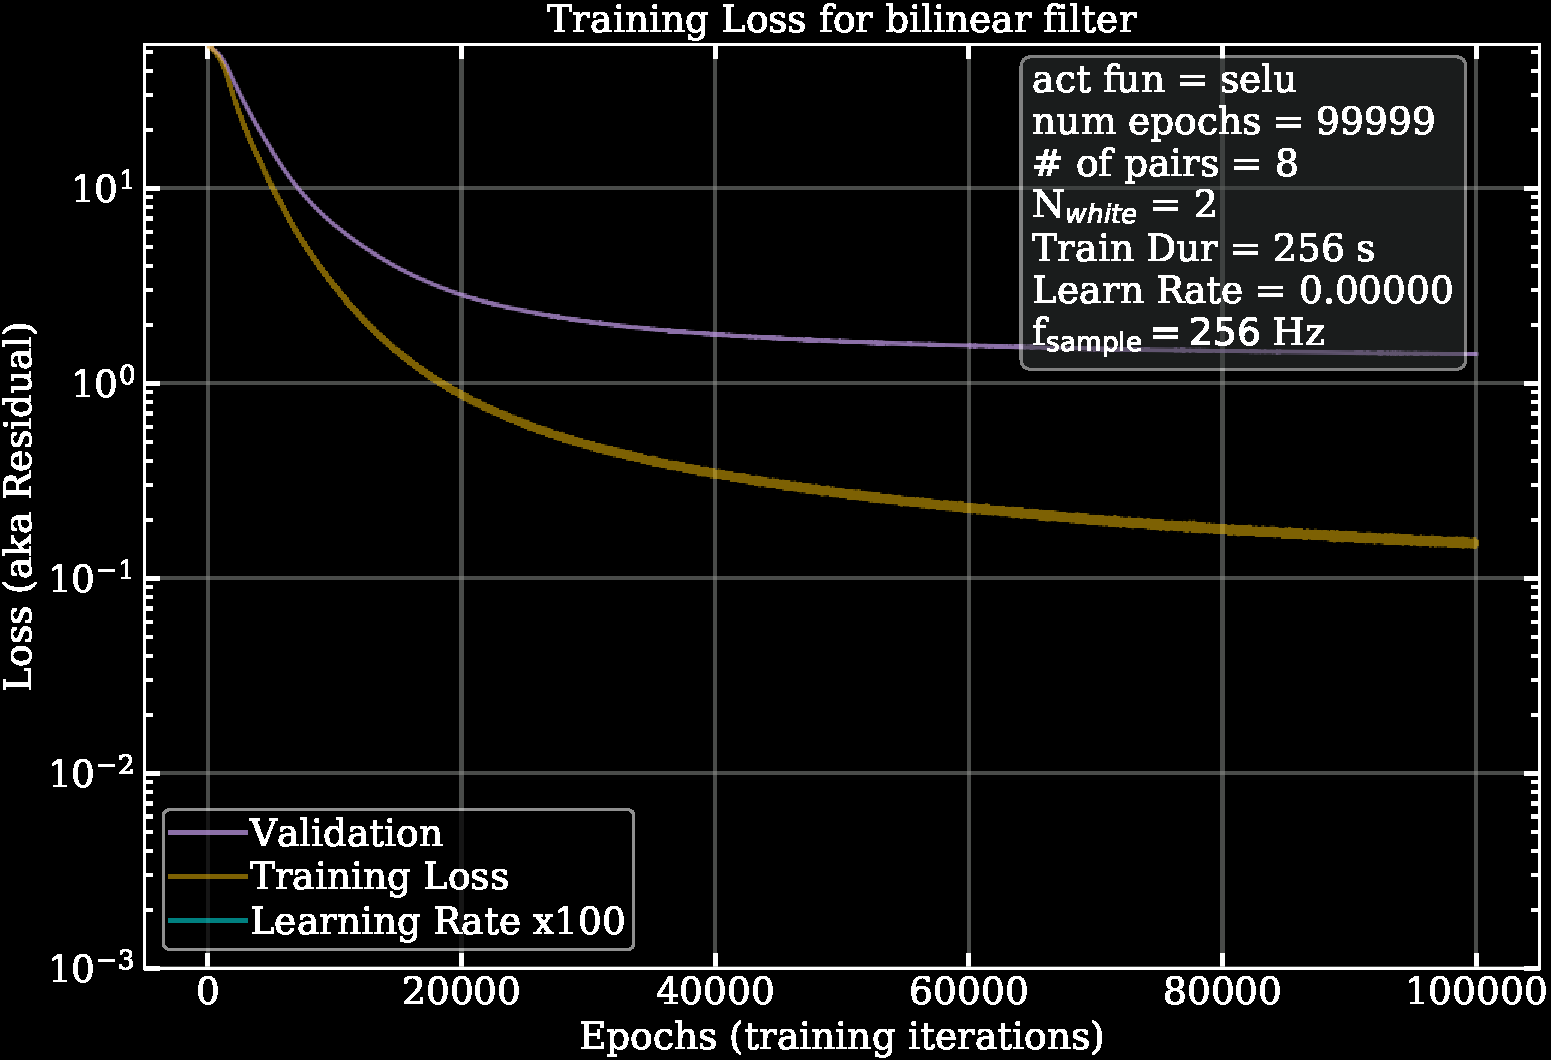
\includegraphics[width=.7\columnwidth]{chapter_noise_sub/etc/loss8C}
   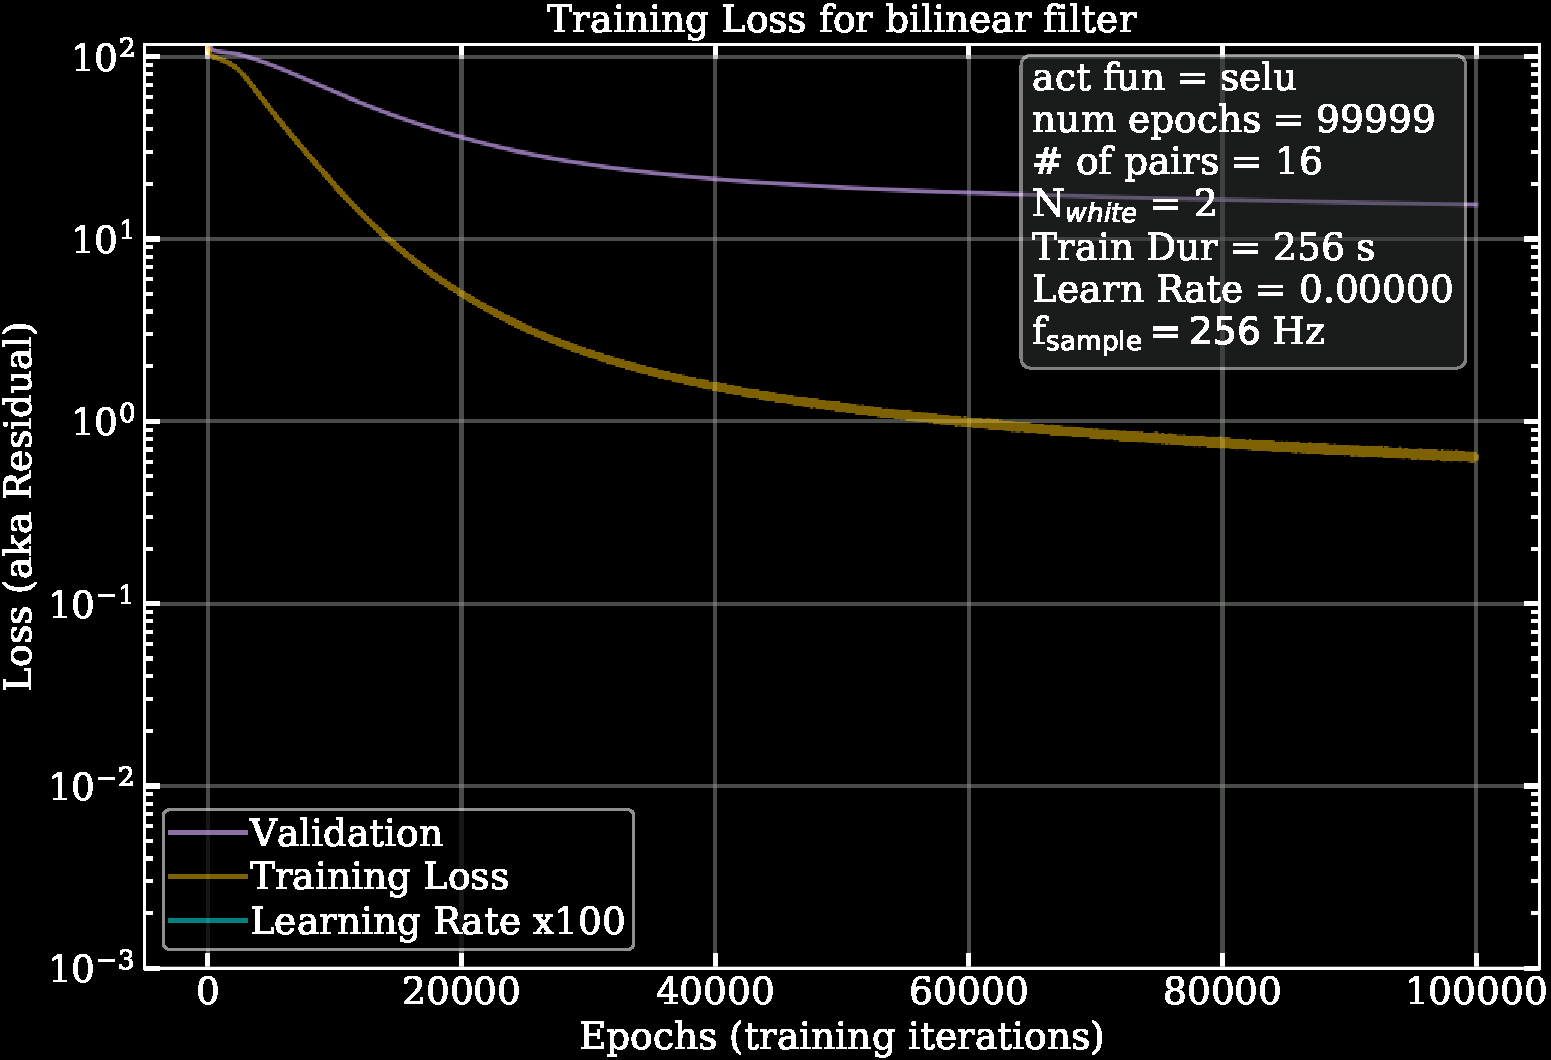
\includegraphics[width=.7\columnwidth]{chapter_noise_sub/etc/loss16C}
   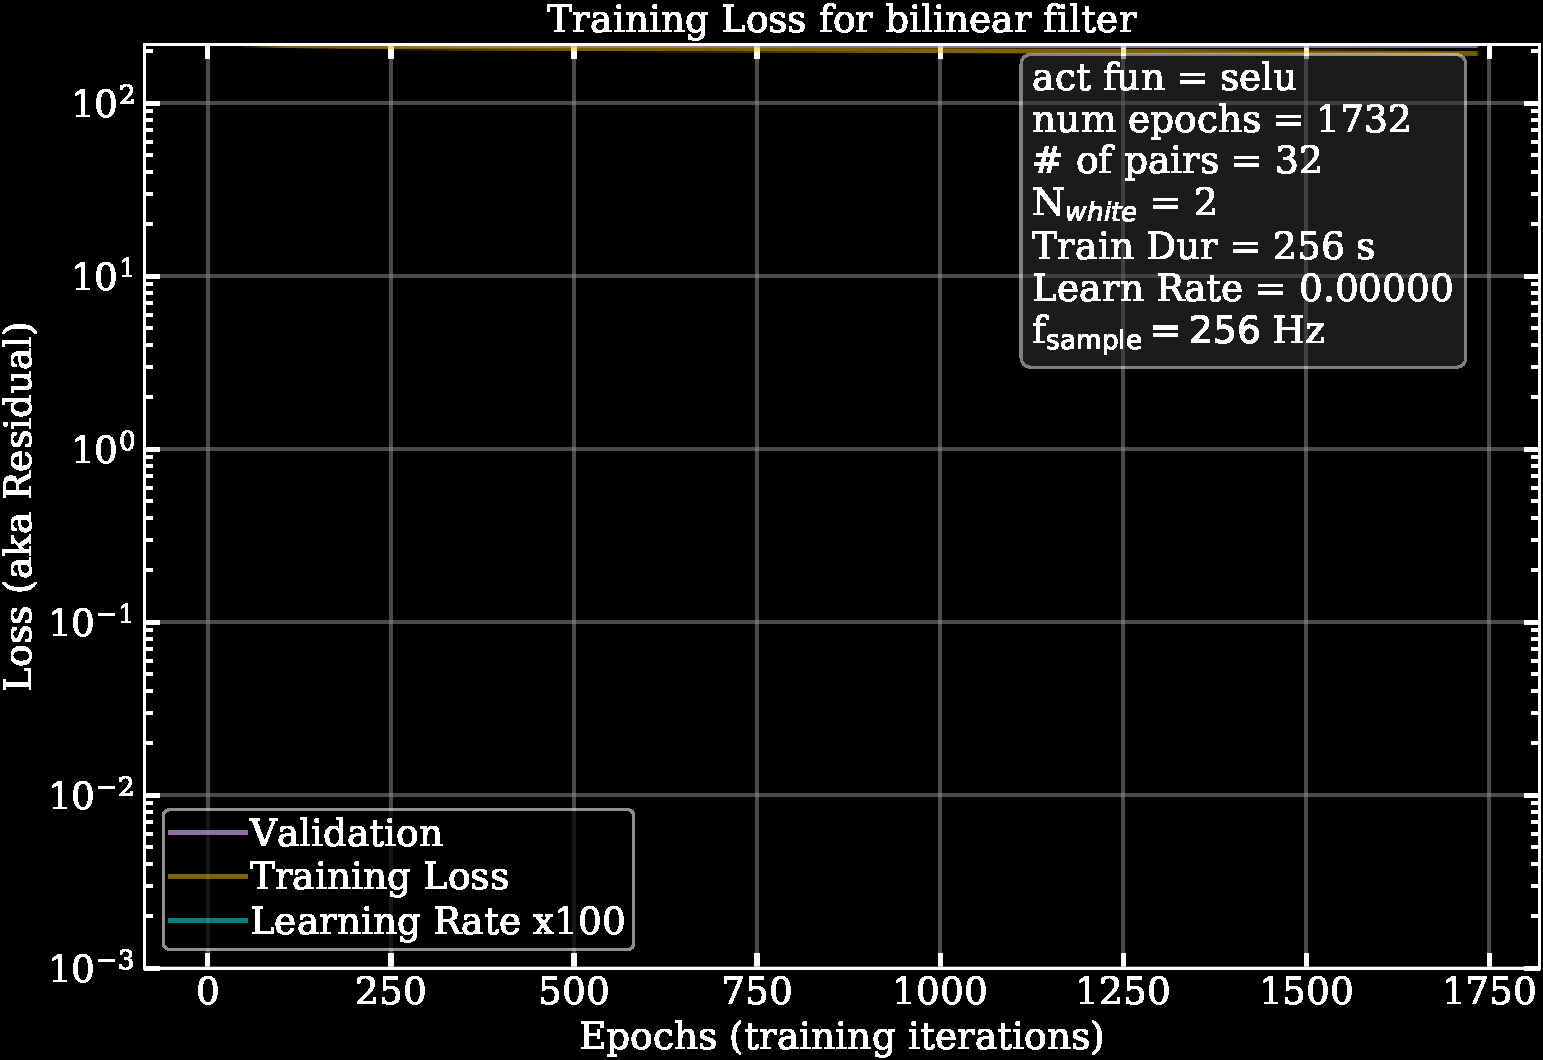
\includegraphics[width=.7\columnwidth]{chapter_noise_sub/etc/loss32C}
   \caption{The loss plotted versus epoch illustrating successful learning for the colored bilinear mock data with 2 (top panel) , 4 (middle panel), and 8 (bottom panel) pairs.}
   \label{fig:loss1}
\end{figure}

%\begin{figure}[htbp]
%   \centering
%   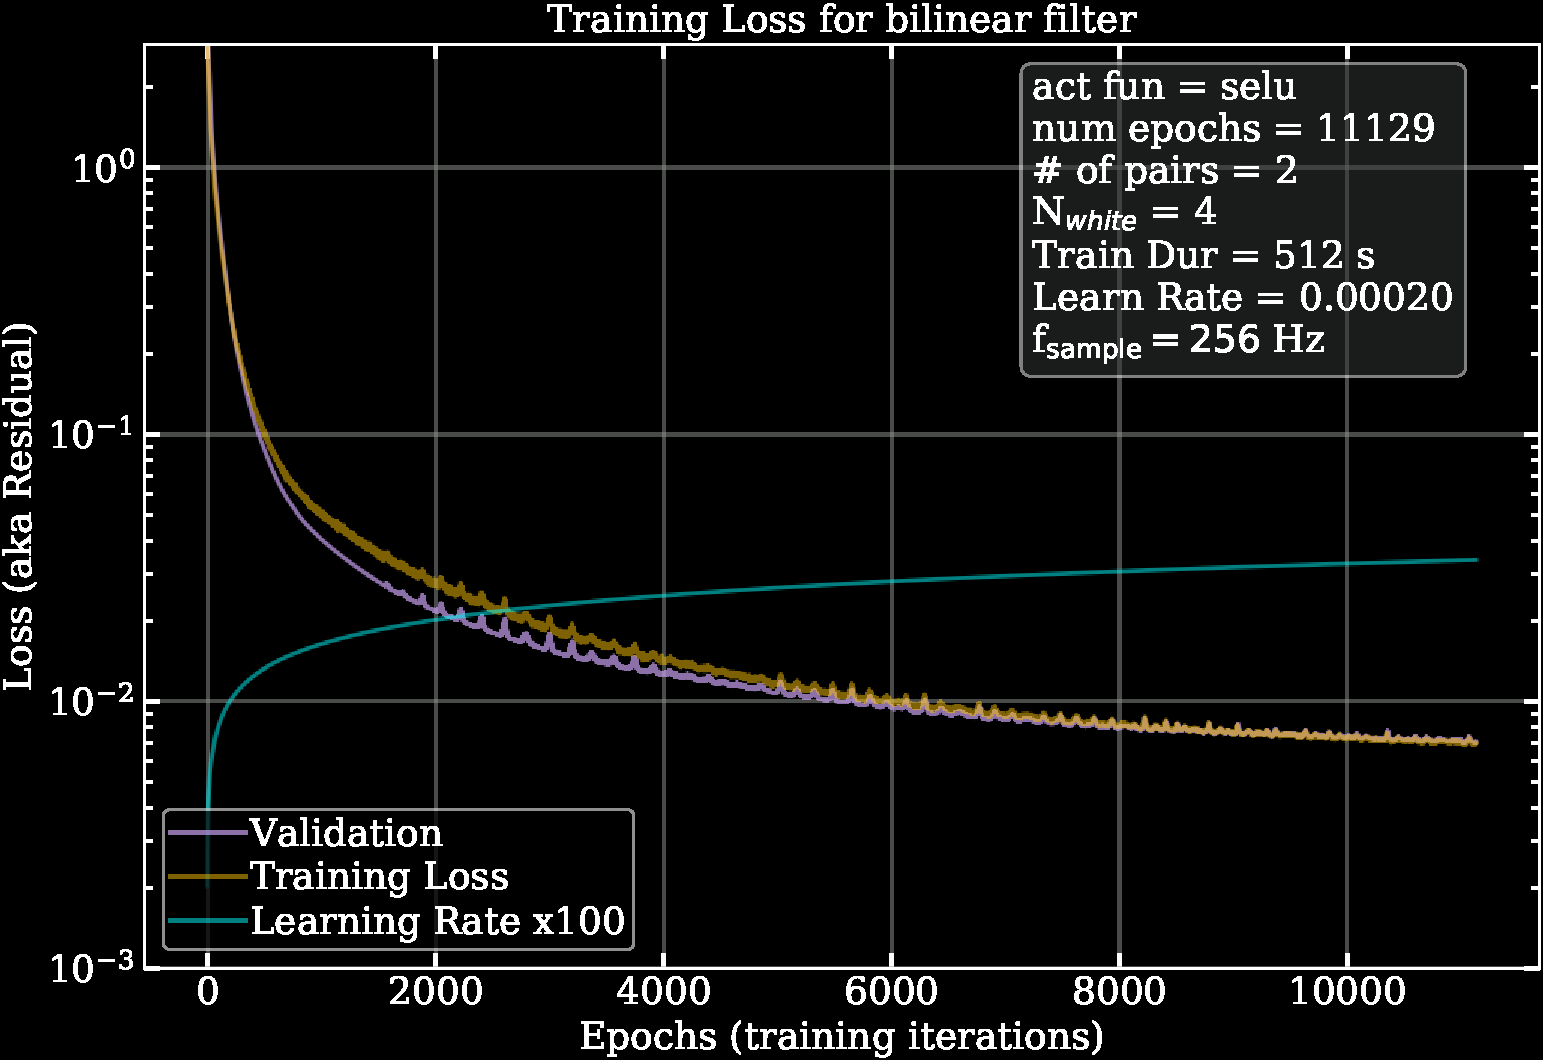
\includegraphics[width=.7\columnwidth]{chapter_noise_sub/etc/loss2}
%   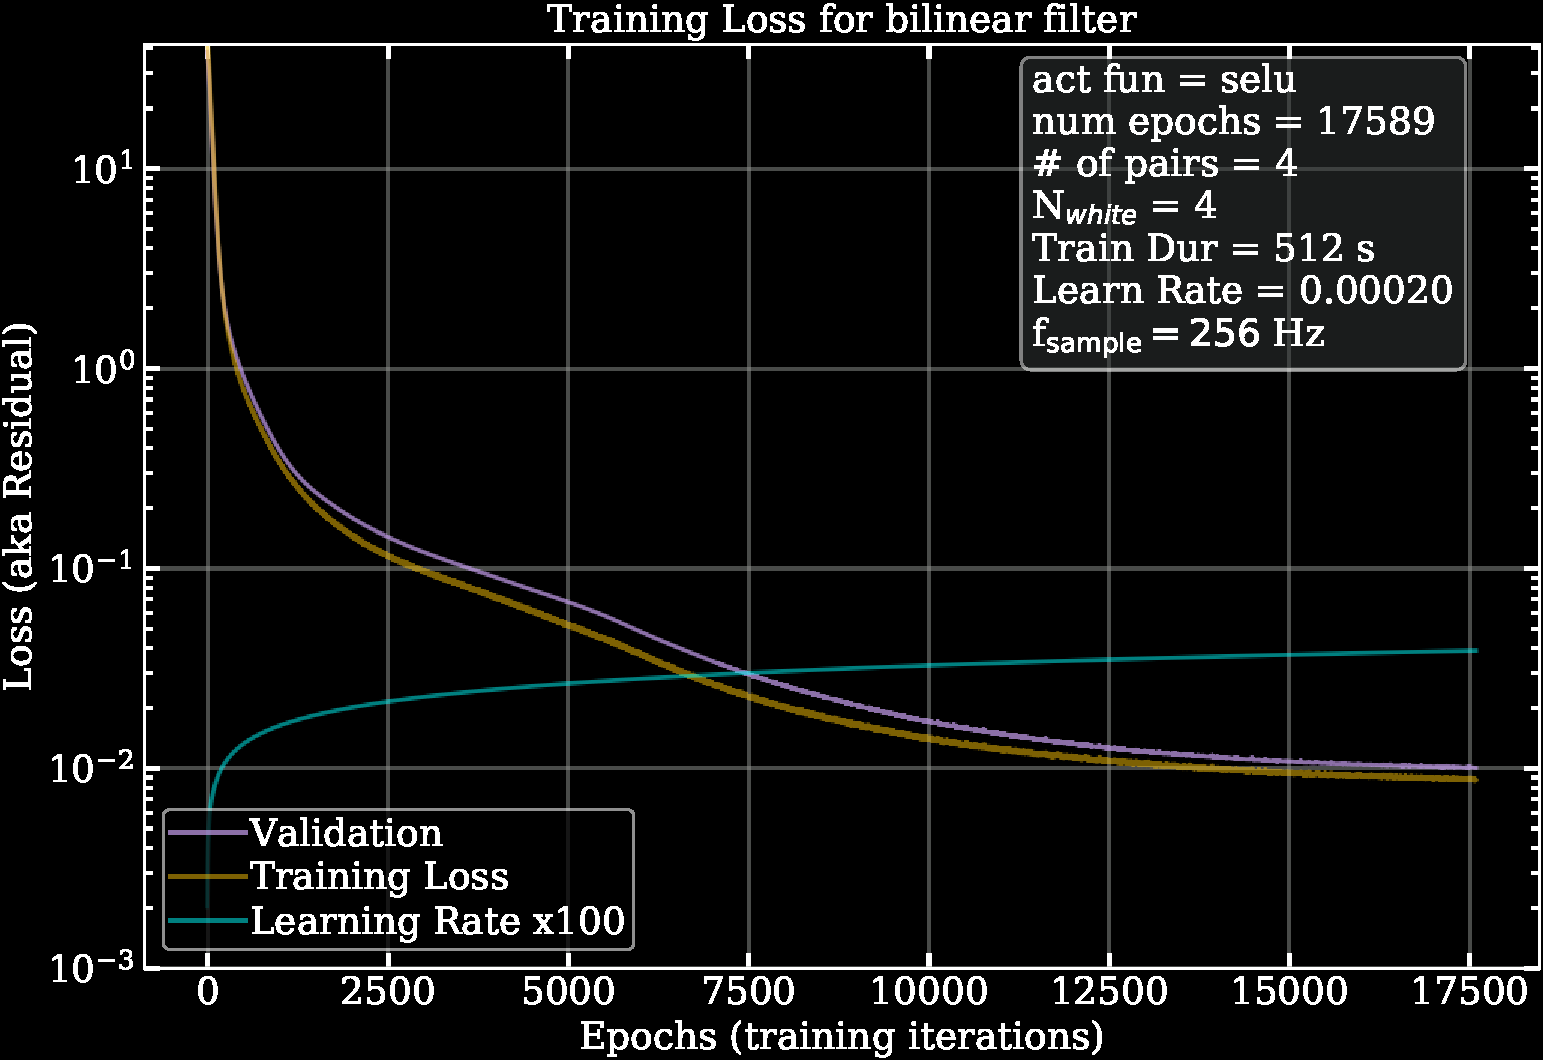
\includegraphics[width=.7\columnwidth]{chapter_noise_sub/etc/loss4}
%   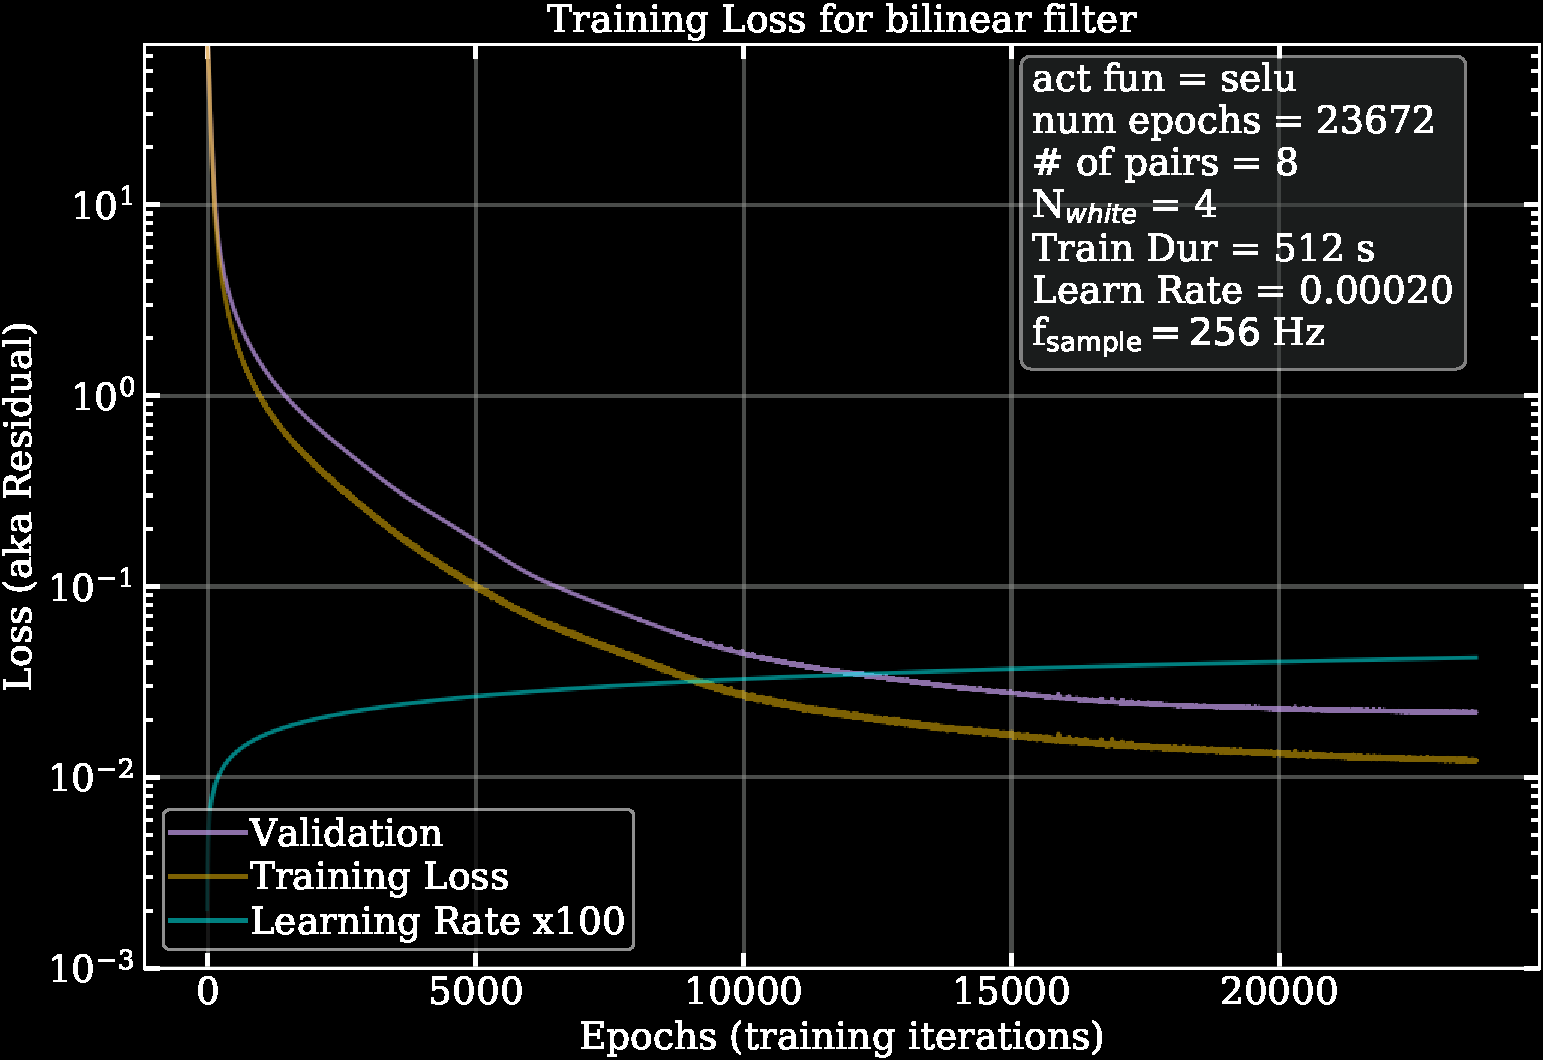
\includegraphics[width=.7\columnwidth]{chapter_noise_sub/etc/loss8}
%   \caption{The loss plotted versus epoch illustrating successful learning for the colored bilinear mock data with 2 (top panel) , 4 (middle panel), and 8 (bottom panel) pairs.}
%   \label{fig:loss1}
%\end{figure}
%
%\begin{figure}[htbp]
%   \centering
%   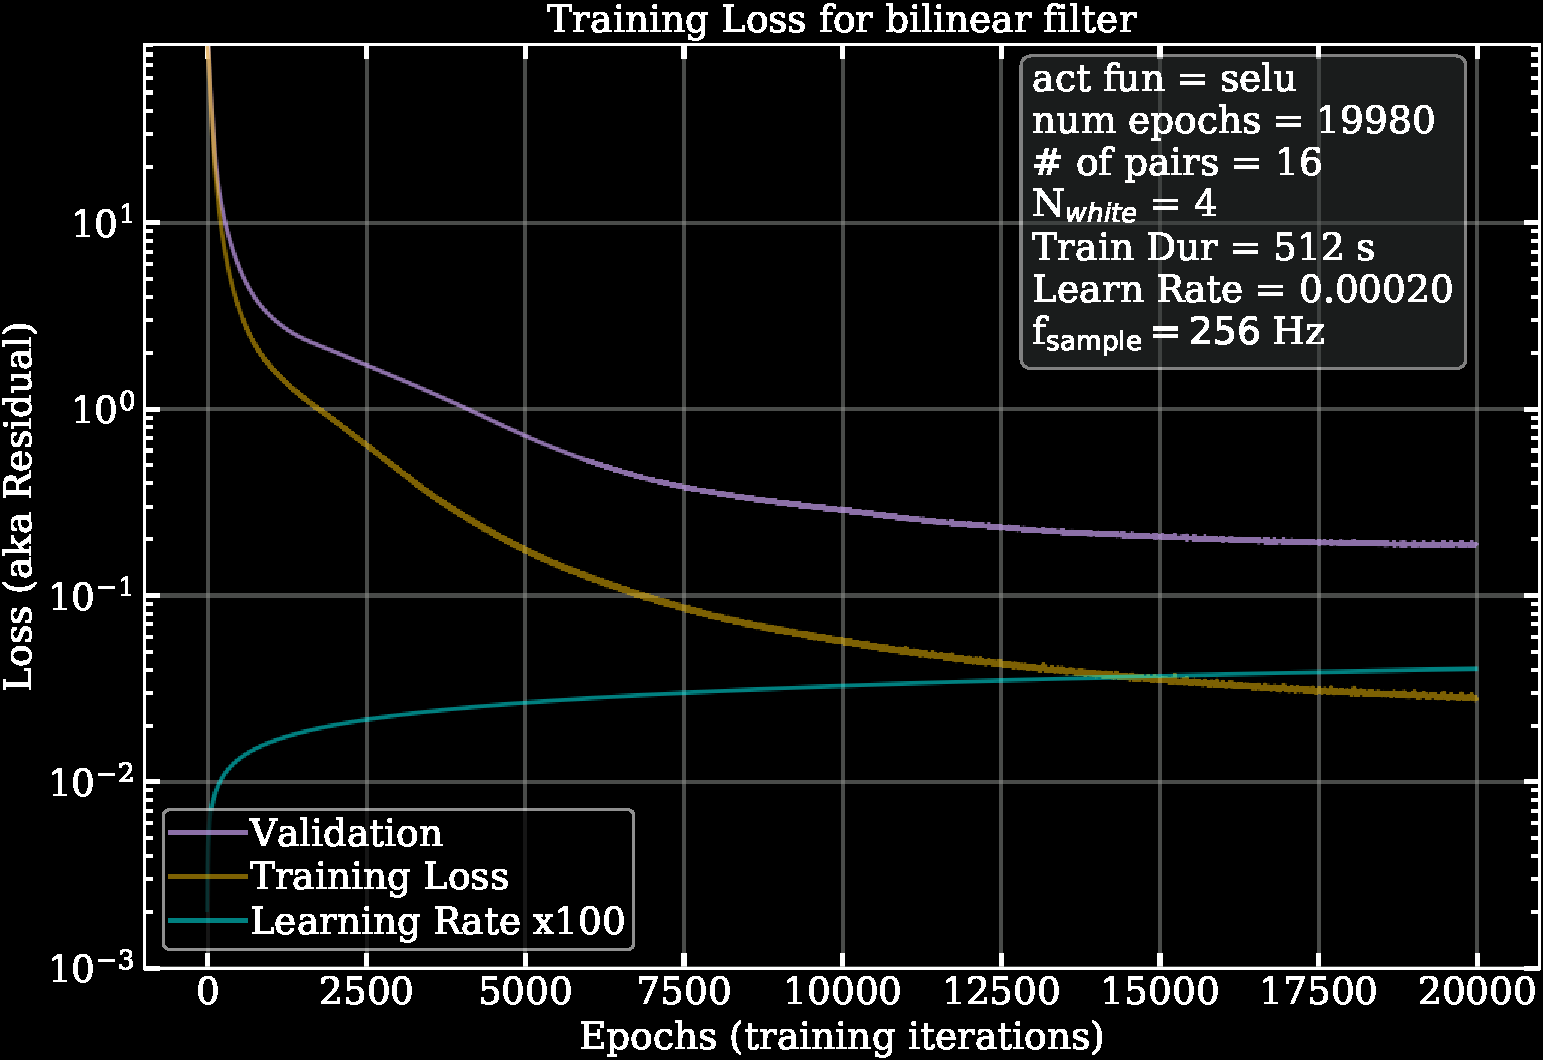
\includegraphics[width=.7\columnwidth]{chapter_noise_sub/etc/loss16}
%   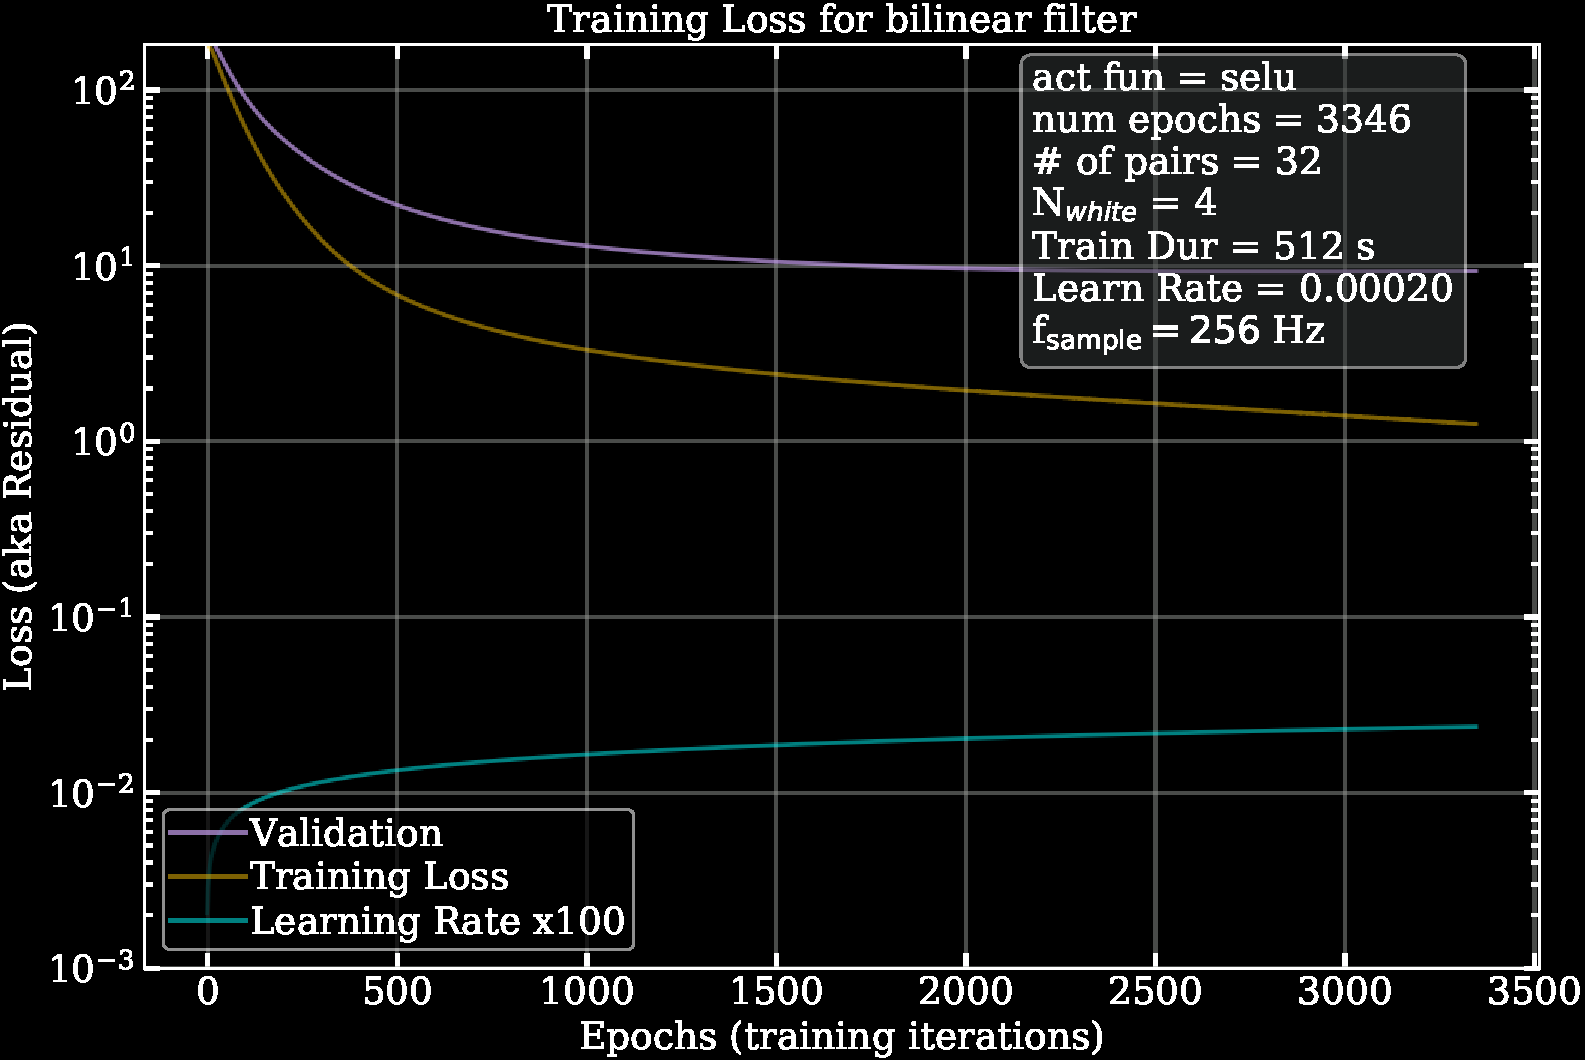
\includegraphics[width=.7\columnwidth]{chapter_noise_sub/etc/loss32}
%   \caption{The loss plotted versus epoch illustrating relatively unsuccessful learning for the colored bilinear mock data with 16 (top panel) and 32 (bottom panel) pairs.}
%   \label{fig:loss2}
%\end{figure}

%\begin{figure}[htbp]
%   \centering
%   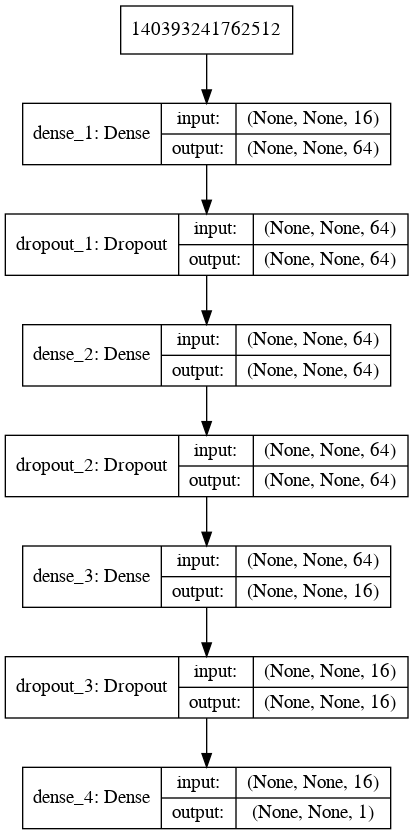
\includegraphics[width=\columnwidth]{chapter_noise_sub/etc/net_diag}
%   \caption{...}
%   \label{fig:net}
%\end{figure}
%
%
%\begin{figure}[htbp]
%   \centering
%   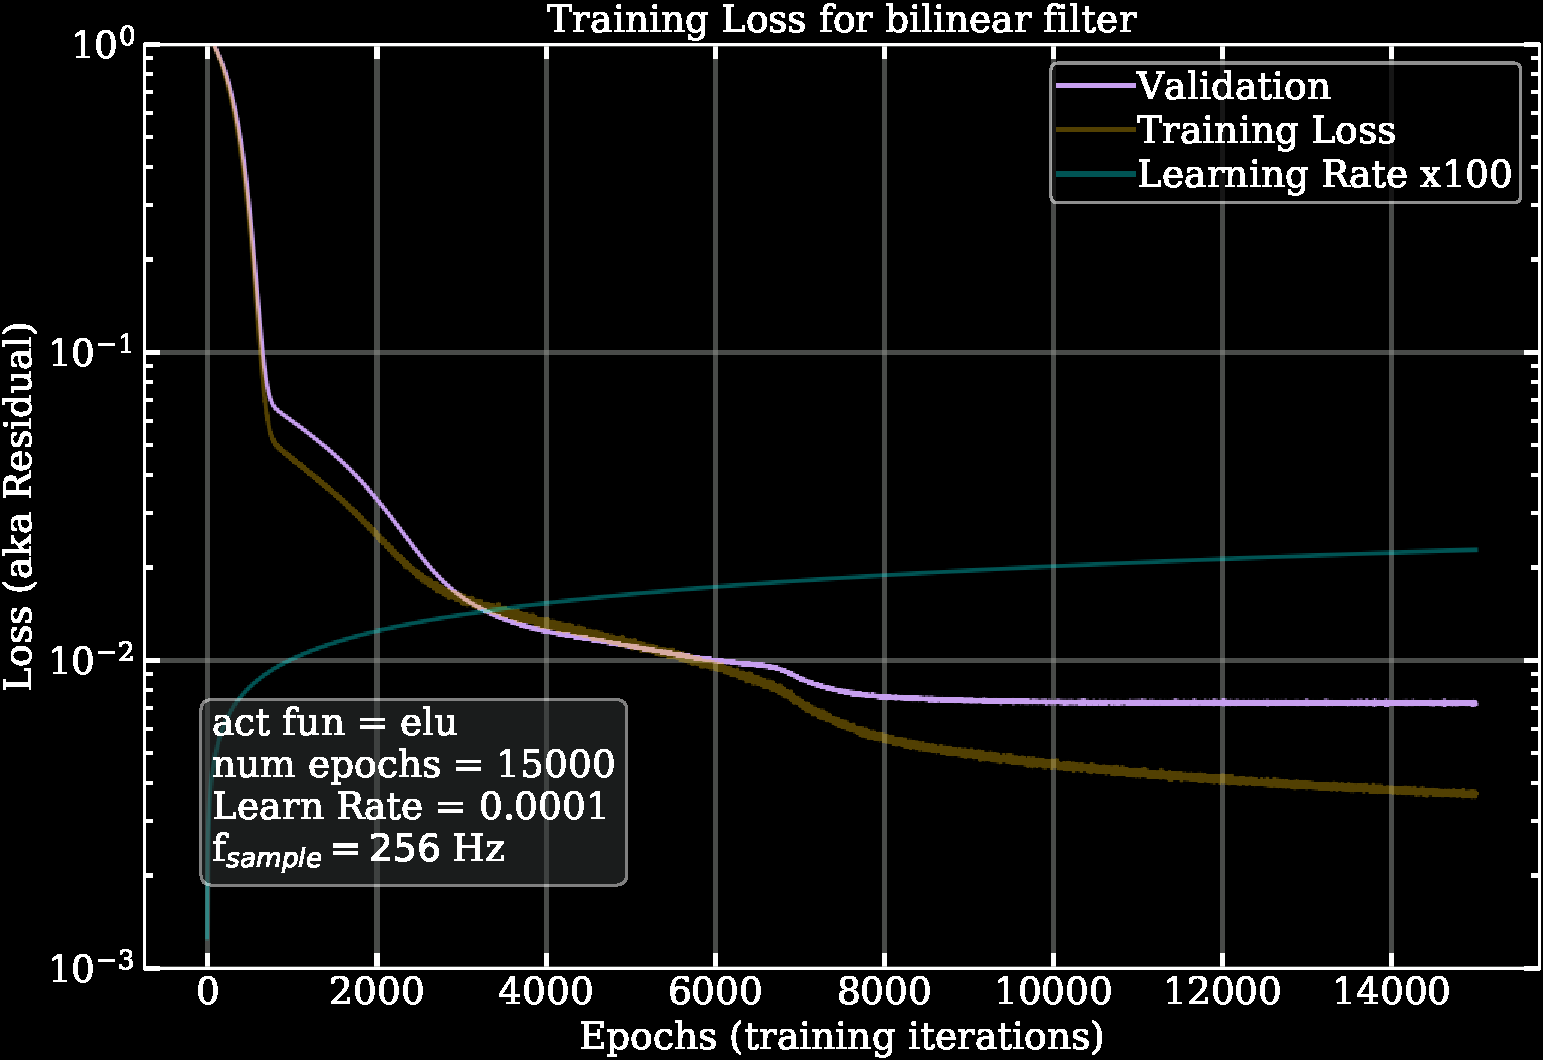
\includegraphics[width=\columnwidth]{chapter_noise_sub/etc/loss_Npairs2}
%   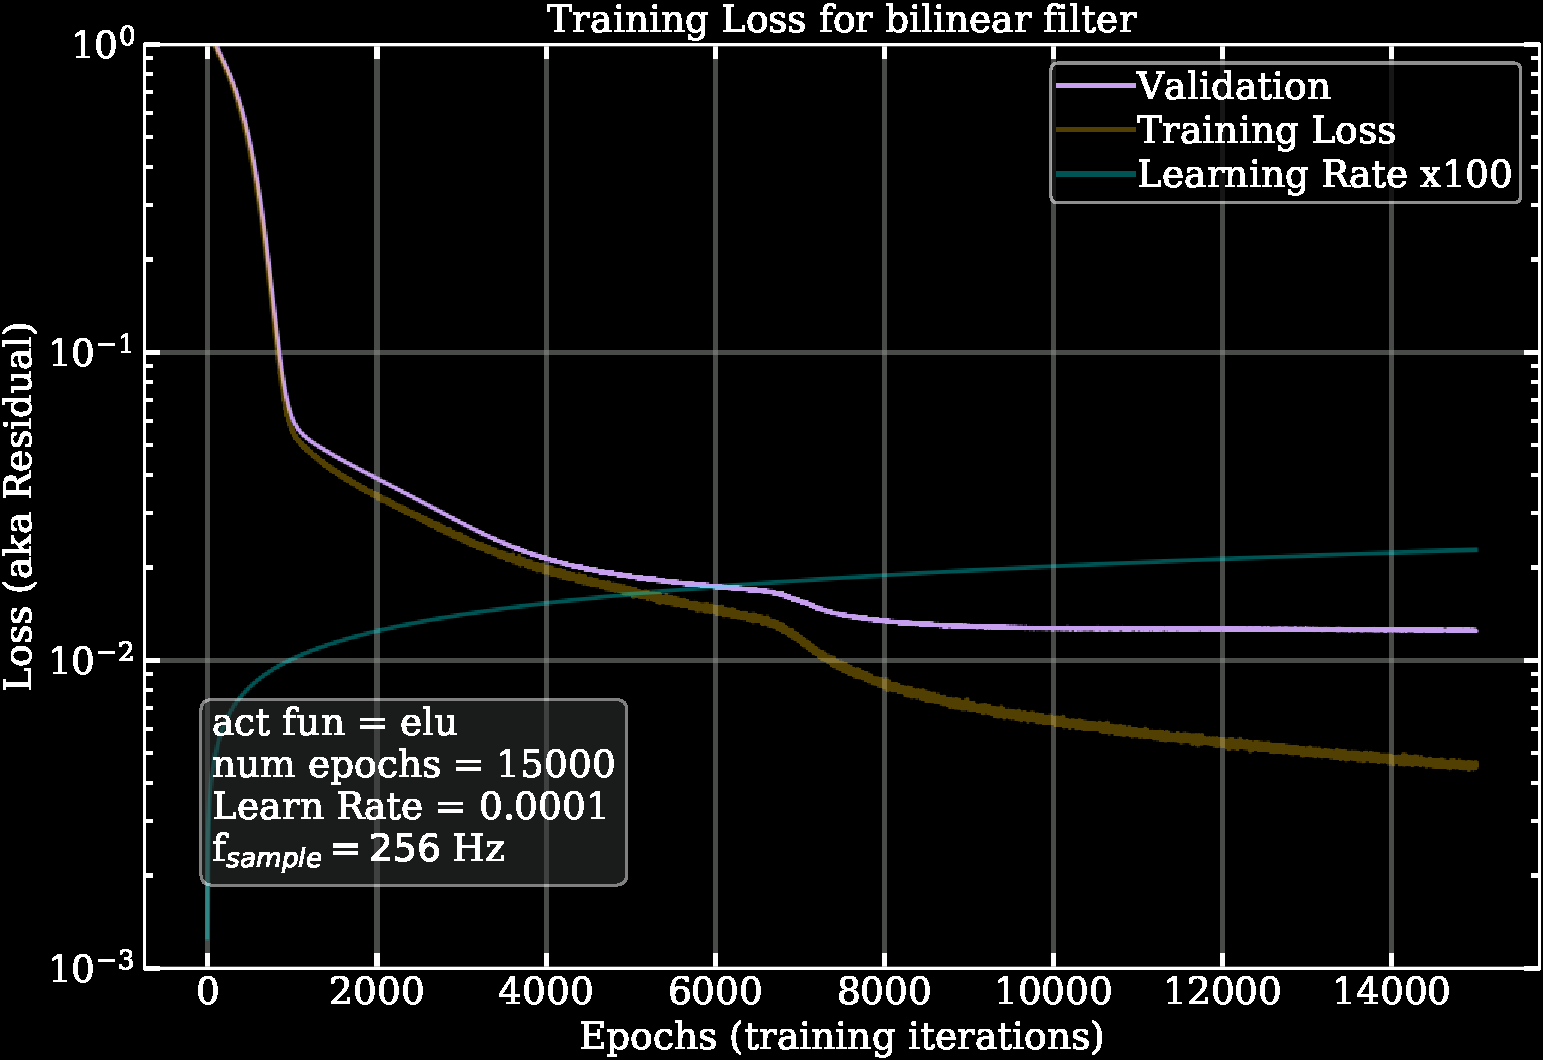
\includegraphics[width=\columnwidth]{chapter_noise_sub/etc/loss_Npairs4}
%   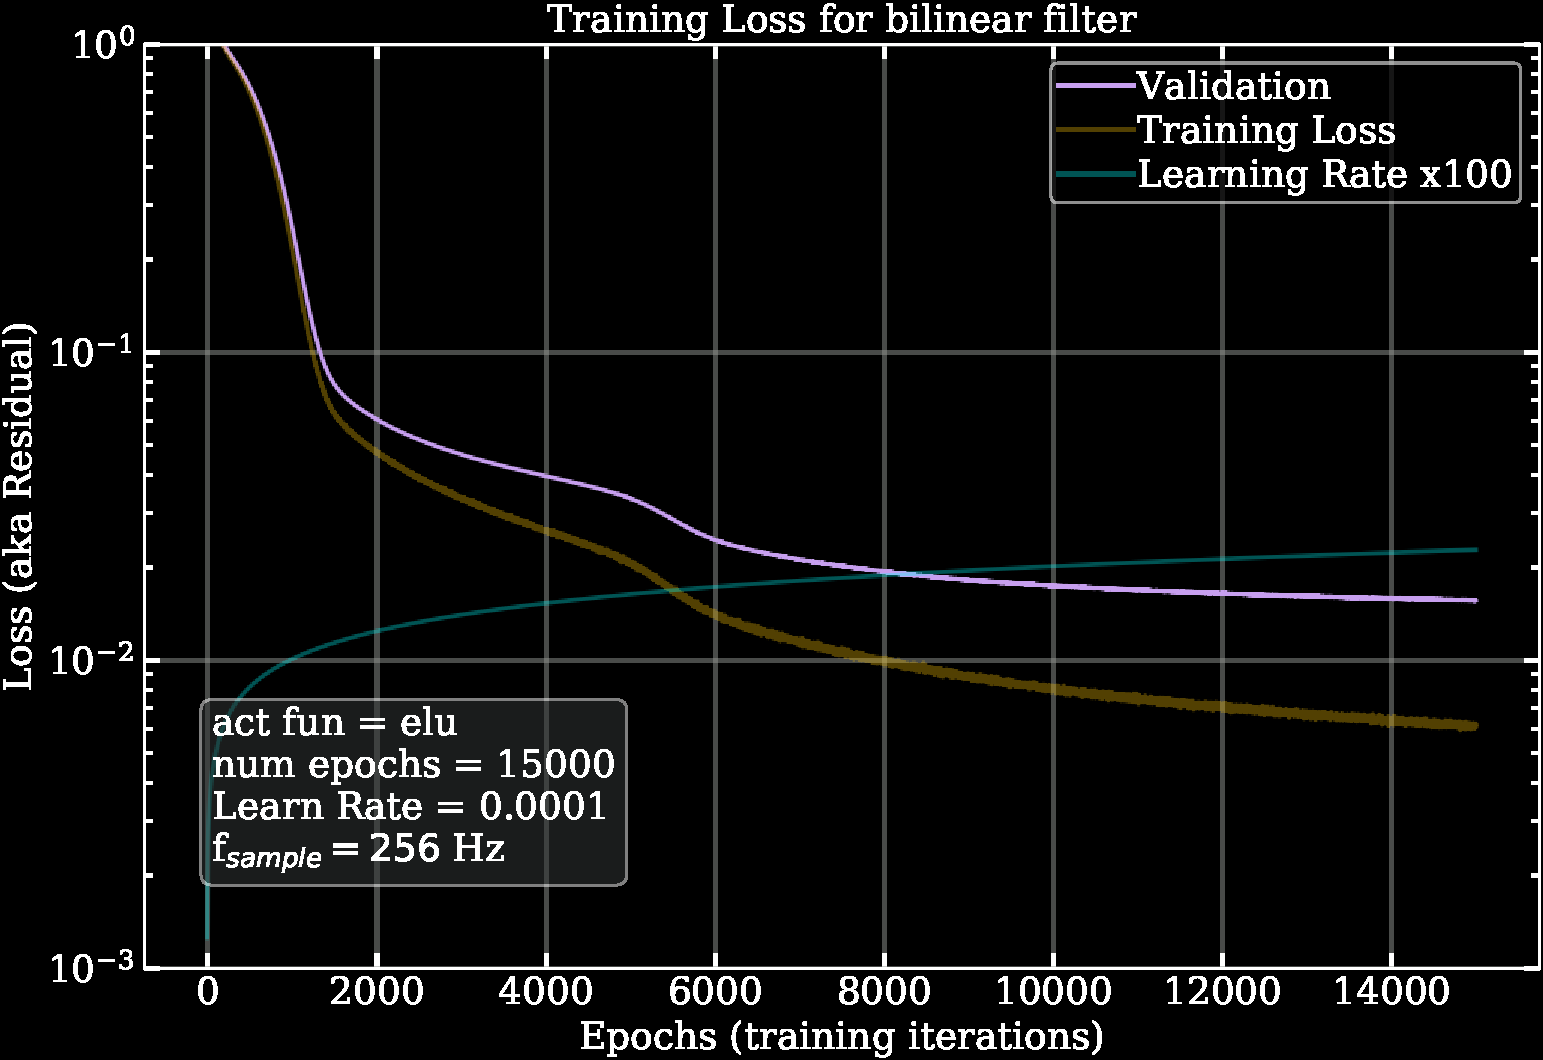
\includegraphics[width=\columnwidth]{chapter_noise_sub/etc/loss_Npairs8}
%   \caption{...}
%   \label{fig:Loss_comp}
%\end{figure}
%
%\begin{figure}[htbp]
%   \centering
%   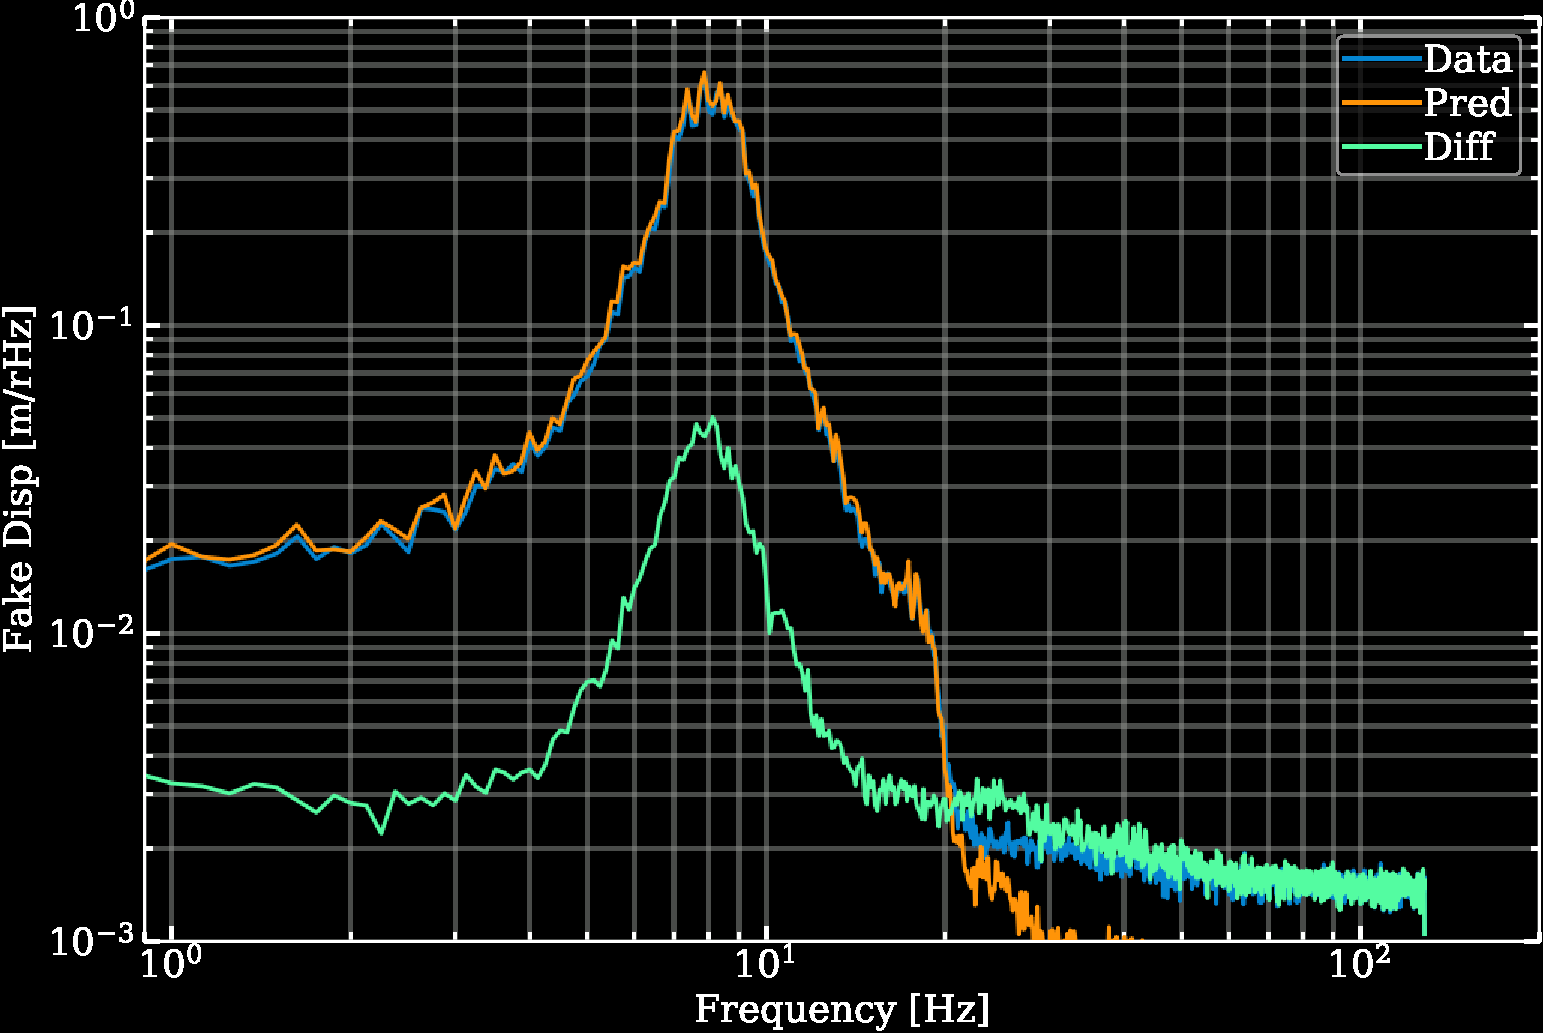
\includegraphics[width=\columnwidth]{chapter_noise_sub/etc/ASD_Npairs2}
%   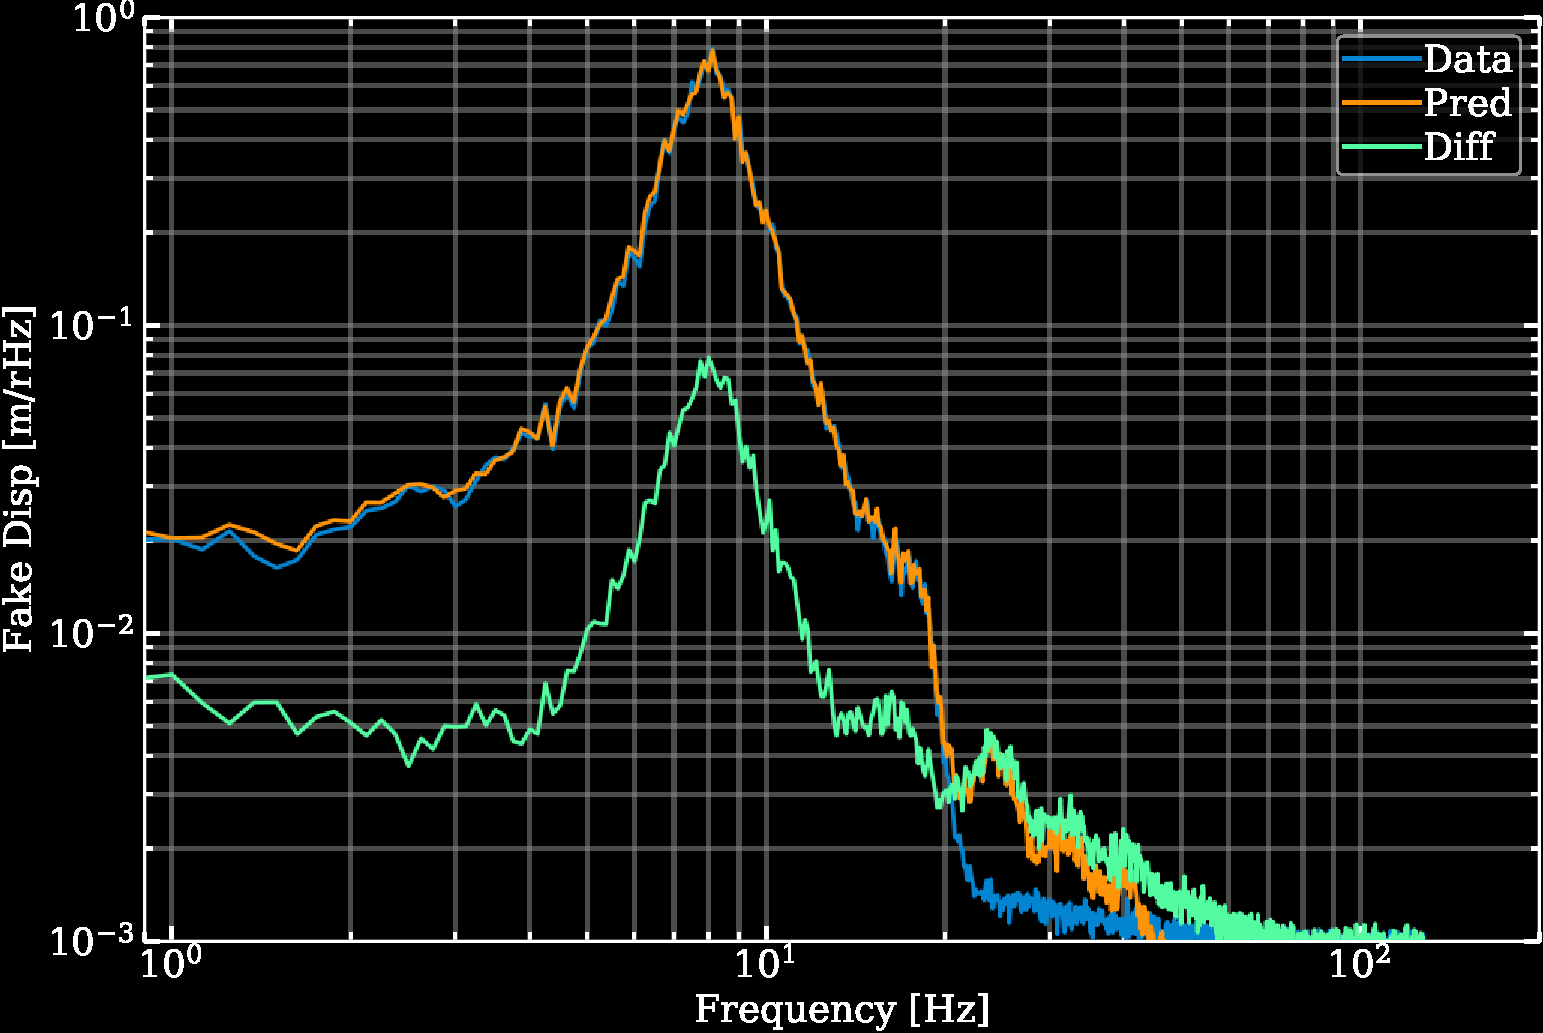
\includegraphics[width=\columnwidth]{chapter_noise_sub/etc/ASD_Npairs4}
%   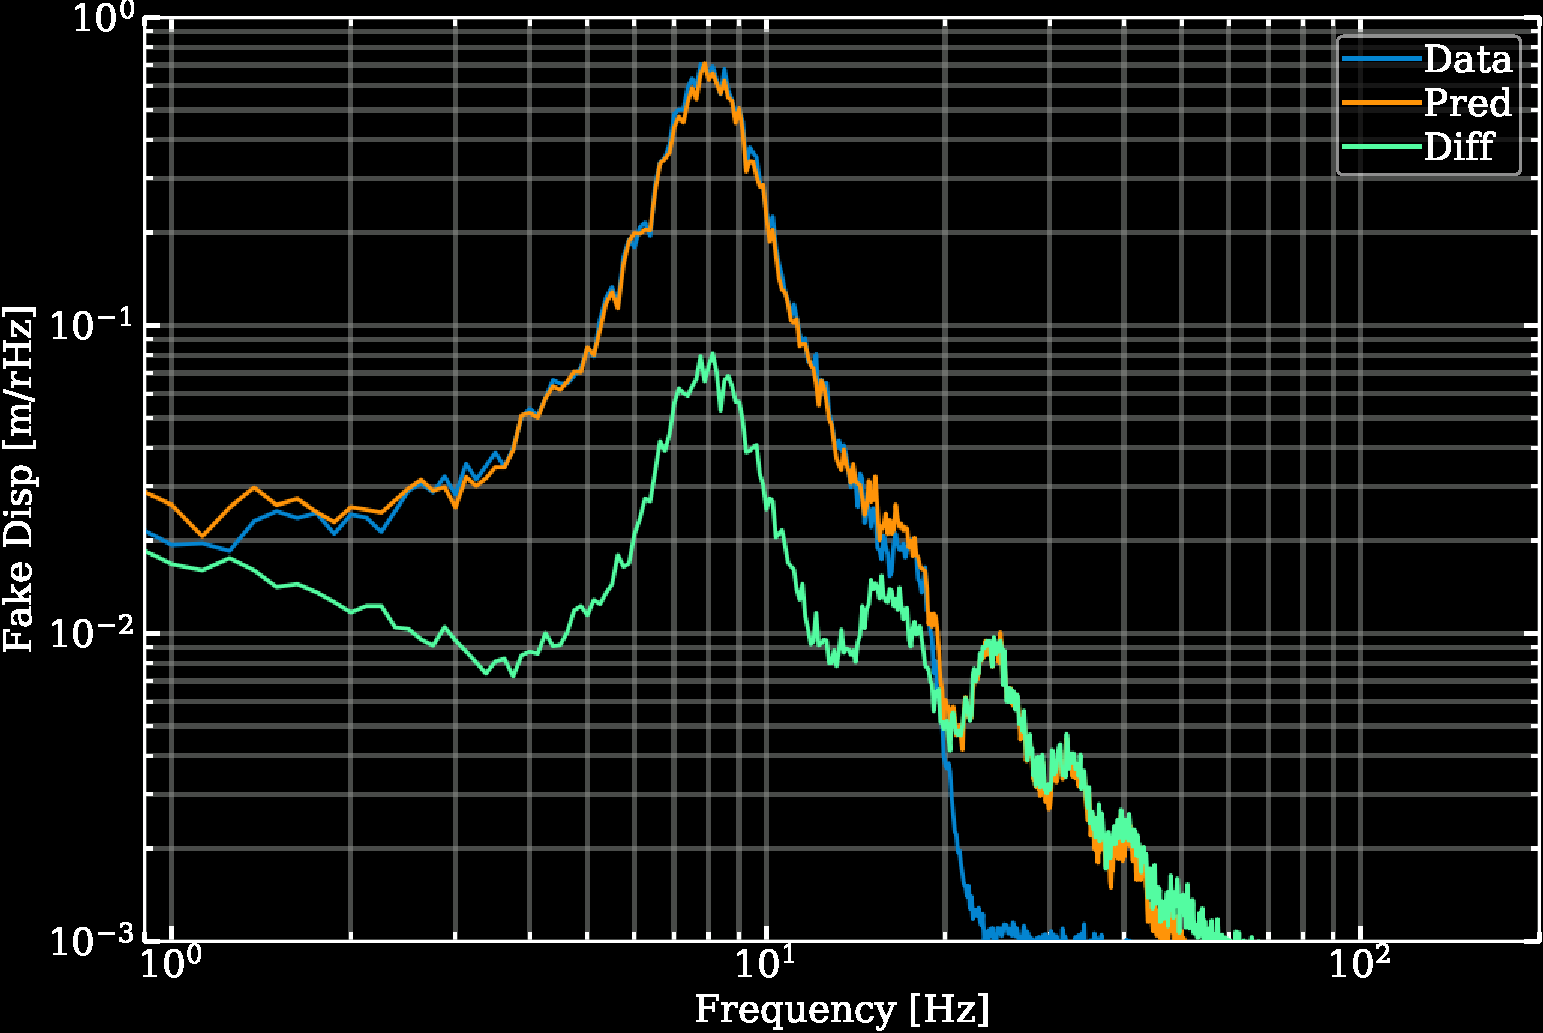
\includegraphics[width=\columnwidth]{chapter_noise_sub/etc/ASD_Npairs8}
%   \caption{...}
%   \label{fig:ASD_comp}
%\end{figure}

\subsection{Bilinear IFO}
We have success solving the most realistic bilinear mock data with a network relying on 1D convolutional layers to learn frequency dependent filtering and EQL layers to learn nonlinear couplings. Figure \ref{fig:ASD} illustrates the successful subtraction 
by showing the amplitude spectral densities of the target, prediction, and residual. Below 20 Hz, we achieve roughly a factor of 3 reduction between the target/neural network prediction and the residual between the target and prediction.

The EQL layers are sandwiched by convolutional layers which have linear activation functions (since the frequency dependent filtering is linear).
A diagram of the specific network that we used is shown in Figure \ref{fig:bifo_net}

\begin{figure}[htbp]
   \centering
   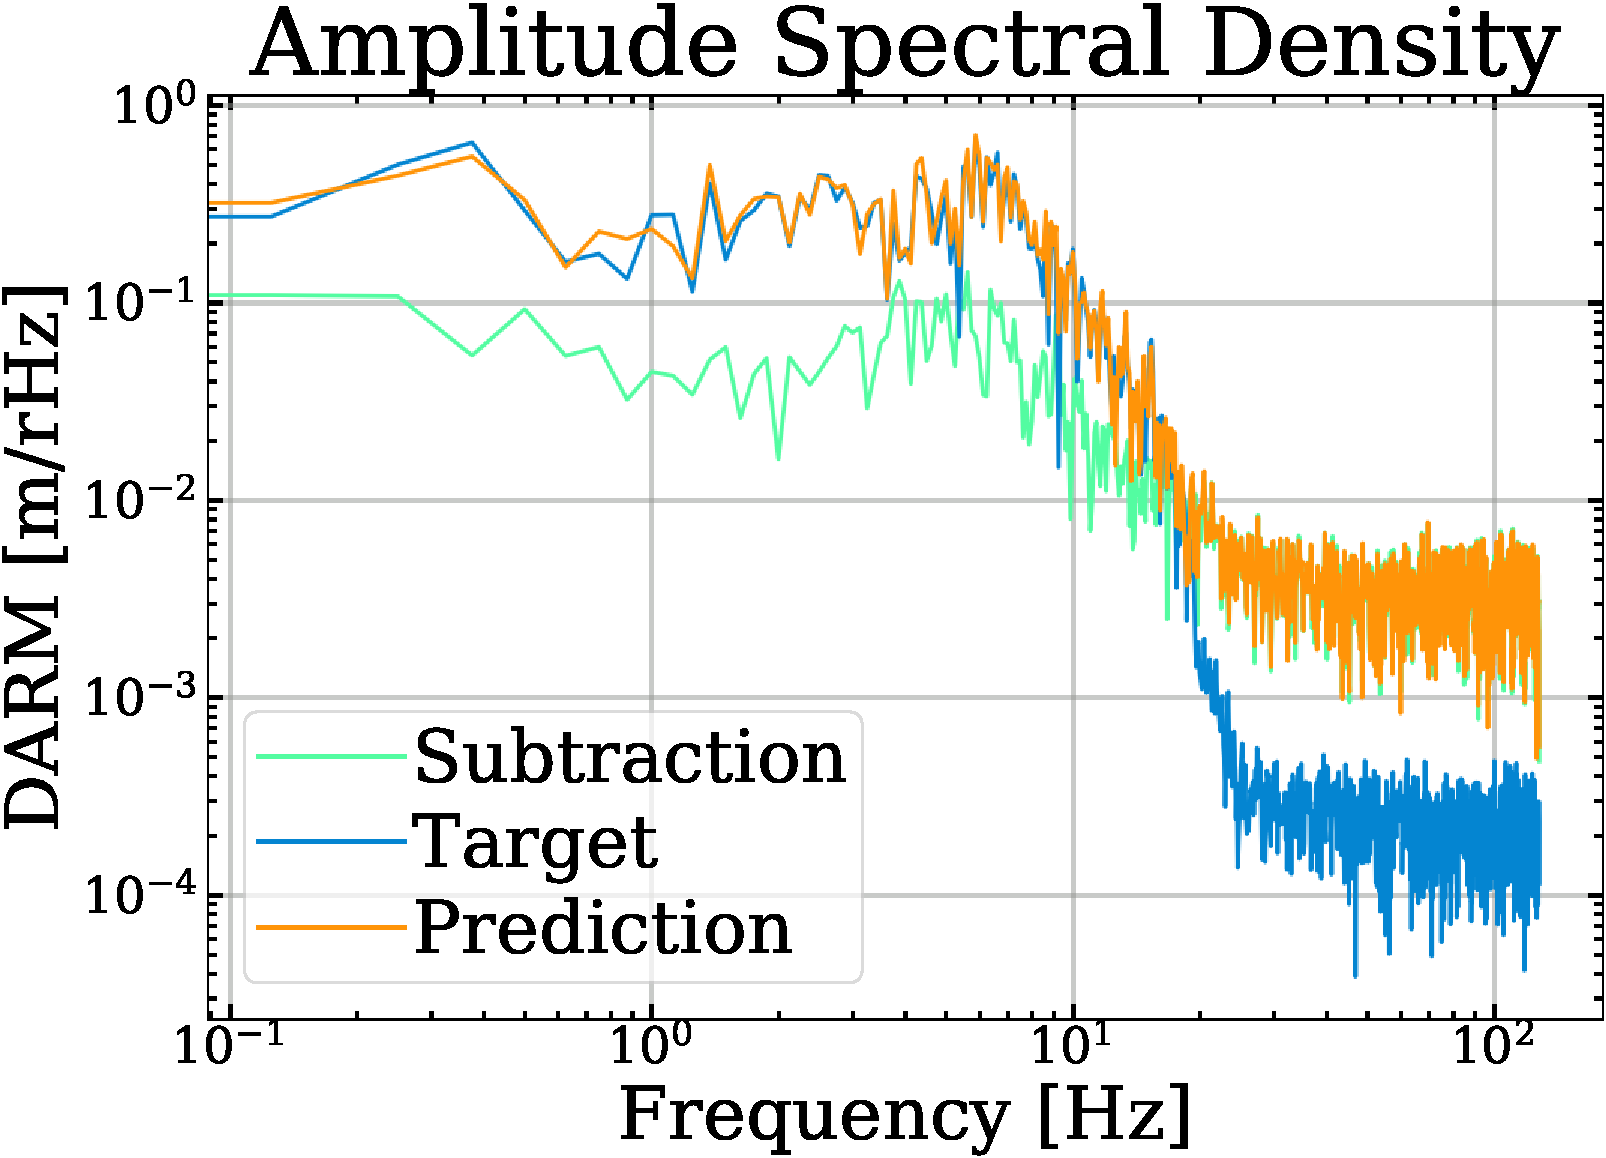
\includegraphics[width=\columnwidth]{chapter_noise_sub/etc/ASD}
   \caption[ASD]{Amplitude Spectral densities illustrating subtraction for the most bilinear IFO mock data. Below 20 Hz, we achieve roughly a factor of 3 reduction between the target/neural network prediction and the residual between the target and prediction}
   \label{fig:ASD}
\end{figure}

\begin{figure}[htbp]
   \centering
   \includegraphics[width=0.7\columnwidth]{chapter_noise_sub/etc/bifo_net}
  \caption{Network schematic for successful network on bilinear IFO mock data.}
   \label{fig:bifo_net}
\end{figure}

\section{Conclusion}

We are actively working on both improving the success on the existing mock data described here and on developing even more realistic mock data. In this work, we present several mock data sets and deep neural networks that have success subtracting noise. In each iteration of mock data, successful networks are designed with the new physics of the iteration in mind.


\printbibliography[heading=subbibliography]
\end{refsection}